\documentclass[11pt,a4paper]{article}

% ---------------------------------------------------------------------------
% Main paper: method and results written as prose, without definitions,
% theorems or proofs. The mathematical results with proofs are collected in
% the separate addendum math_addendum.tex. Results: HyperCloudCore 0.7.8.
% ---------------------------------------------------------------------------

% ---------------------------------------------------------------------------
% Packages
% ---------------------------------------------------------------------------
\usepackage[margin=2.5cm]{geometry}
\usepackage[utf8]{inputenc}
\usepackage{amsmath,amssymb,amsthm,mathtools}
\usepackage{bm}
\usepackage{graphicx}
\usepackage{booktabs}
\usepackage{array}
\usepackage{xcolor}
\usepackage{tikz}
\usetikzlibrary{arrows.meta,calc,decorations.pathreplacing}
\usepackage{algorithm}
\usepackage{algpseudocode}
\usepackage{enumitem}
\usepackage{caption}
\usepackage{subcaption}
\usepackage[numbers,sort&compress]{natbib}
\usepackage{microtype}
\usepackage{authblk}
\usepackage[section]{placeins}% floats are output before the next section starts
\usepackage[colorlinks=true,linkcolor=blue!50!black,citecolor=green!35!black,urlcolor=blue!60!black]{hyperref}
\usepackage[capitalise,nameinlink]{cleveref}

\captionsetup{font=small,labelfont=bf}
\setlist{itemsep=2pt,topsep=4pt}

% Float placement: allow larger floats at the top of text pages and fuller float
% pages, so that figures and tables stay close to the text that cites them.
\renewcommand{\topfraction}{0.85}
\renewcommand{\bottomfraction}{0.6}
\renewcommand{\textfraction}{0.12}
\renewcommand{\floatpagefraction}{0.75}
\setcounter{topnumber}{3}
\setcounter{bottomnumber}{2}
\setcounter{totalnumber}{5}

% ---------------------------------------------------------------------------
% Macros
% ---------------------------------------------------------------------------
\numberwithin{equation}{section}

\crefname{assumption}{Assumption}{Assumptions}
\crefname{algorithm}{Algorithm}{Algorithms}

\newcommand{\R}{\mathbb{R}}
\newcommand{\N}{\mathbb{N}}
\newcommand{\dd}{\mathrm{d}}
\newcommand{\nb}{\nu}
\newcommand{\cnb}{\bar\nu}
\newcommand{\Ad}{\mathcal{G}}
\newcommand{\Lop}{\mathcal{L}}
\newcommand{\Dop}{\mathcal{D}}
\newcommand{\Fs}{F^{*}}
\newcommand{\ptil}{\tilde p}
\newcommand{\Ntil}{\tilde N}
\newcommand{\sgn}{\operatorname{sign}}
\newcommand{\ord}[2]{k_{#1\to #2}}
\newcommand{\qdiv}{q}
\newcommand{\CFL}{\mathrm{CFL}}

\definecolor{lowc}{RGB}{200,30,30}
\definecolor{highc}{RGB}{170,170,170}

% ---------------------------------------------------------------------------
\title{High-order meshfree MUSCL schemes with a~posteriori\\
order detection for hyperbolic systems\\ on scattered point clouds}
\author[1]{Pascal Jung}
\author[1,2]{Klaas Willems}
\author[1]{Axel Klar}
\affil[1]{Faculty of Mathematics, RPTU Kaiserslautern-Landau, Kaiserslautern, Germany}
\affil[2]{Department of Computer Science, KU Leuven, Leuven, Belgium}
\date{30~October 2026}

\begin{document}
\maketitle

\begin{abstract}
We present meshfree MUSCL schemes of arbitrary design order $k$ for hyperbolic systems of conservation laws on scattered point clouds. Moving least-squares (MLS) reconstructions of degree $k-1$ are evaluated at the midpoints between neighbouring particles, the jumps are resolved by approximate Riemann solvers, and the interface fluxes are differentiated by an MLS derivative operator whose weights sum to zero. The scheme is exact for polynomial solutions of linear problems, is consistent of order $k$ on periodic Cartesian lattices, and its conservation error is the lack of antisymmetry of the derivative weights. Orienting the dissipation of the Rusanov flux by the signs of the derivative weights keeps density and pressure positive in the first-order fallback scheme for derivative operators of any degree. The degree of the derivative operator can therefore stay fixed while MOOD lowers only the degree of the reconstructions. Discontinuities are treated by slope limiters or by a per-particle MOOD procedure within SSP Runge--Kutta methods. Numerical experiments confirm the design orders up to five for smooth solutions on regular and perturbed clouds and show that, with a derivative operator of degree one, the conservation defect at moving shocks decreases under refinement. Two-dimensional shock problems up to the double Mach reflection and the Mach~3 forward-facing step are computed robustly with positive density and pressure. A smooth-extremum detection adapted to meshfree stencils prevents MOOD from clipping the core of an isentropic vortex for orders three and four once the core is resolved by ten to twenty particles per radius.
\end{abstract}

\noindent\textbf{Keywords:} meshfree methods; generalized finite differences; moving least squares; MUSCL; MOOD; a~posteriori limiting; compressible Euler equations; point clouds

% ===========================================================================
\section{Introduction}\label{sec:intro}
% ===========================================================================

Hyperbolic systems of conservation laws describe the transport of mass, momentum and energy in compressible flows and many other applications. Their solutions develop discontinuities in finite time, and robust high-resolution discretizations are assembled from a few well-understood ingredients: a conservative flux form, upwinding through exact or approximate Riemann solvers, high-order reconstructions, and a mechanism that suppresses spurious oscillations at discontinuities \cite{vanLeer1979,Harten1987,Shu1998,Toro2009}. In finite volume (FV) and discontinuous Galerkin methods all of these ingredients rest on a mesh: the faces of the control volumes carry the numerical fluxes, the telescoping sum of the fluxes gives discrete conservation, and the cells define the stencils of the reconstruction.

Meshfree methods replace the mesh by a cloud of points, which we call particles, and approximate derivatives from local neighbourhoods. Generalized finite difference methods (GFDM) \cite{Jensen1972,Perrone1975} approximate derivatives from Taylor expansions on local stars of points; since Liszka and Orkisz \cite{Liszka1980} they use weighted least-squares fits of local polynomials \cite{Benito2001,Benito2007}, as do the finite pointset method \cite{Tiwari2003} and moving least-squares (MLS) approximations \cite{Lancaster1981,Levin1998}; see \cite{Belytschko1996,Nguyen2008} for reviews, \cite{Seibold2006} for stencil properties and \cite{Clain2024} for very high-order variants. Since a point cloud needs no connectivity, meshfree methods are attractive for complex and moving geometries, where generating and maintaining a mesh dominates the cost of a simulation.

For hyperbolic problems the mesh-based ingredients do not carry over directly. Central meshfree differentiation is unstable for advection on irregular clouds and requires upwinding or artificial dissipation \cite{FornbergLehto2011,Willems2025}. Shocks require non-oscillatory and positivity-preserving mechanisms that work on irregular and overlapping stencils. And without faces there is no telescoping sum of fluxes, so discrete conservation is not automatic; convergent conservative schemes converge to weak solutions \cite{LaxWendroff1960}, whereas non-conservative schemes may converge to discontinuities that move with wrong speeds \cite{HouLeFloch1994}.

Several lines of work address these issues. Kinetic upwinding on least-squares stencils leads to the least-squares kinetic upwind method \cite{Ghosh1995,Ramesh2001}, and positivity can be obtained by upwinding and dissipation \cite{Chandrashekar2004}. Conservation has been addressed by meshless ``face'' coefficients that are antisymmetric and satisfy a closure condition \cite{Chiu2011,Chiu2012}, by least-squares methods that enforce the closure condition \cite{Huh2018}, by a GFDM that conserves fluxes approximately over closed local cells \cite{Suchde2017,SuchdeThesis2018}, and by meshless volume schemes, which are, however, not formally conservative \cite{Katz2009}. High-order non-oscillatory reconstructions have been transferred to particle methods through MLS-based WENO schemes \cite{Avesani2014}. Most closely related to the present work, Willems, Klar and Samaey \cite{Willems2025,WillemsCode2025} proposed meshless MUSCL schemes for linear advection in which reconstructed values at the midpoints between neighbouring particles are differentiated with a factor two, and in which spurious oscillations are removed by Multi-dimensional Optimal Order Detection (MOOD). On irregular clouds these schemes were found to be considerably more reliable than meshless WENO schemes. A follow-up work applies a meshless MUSCL method with MOOD to the nonlinear BGK equation on moving clouds \cite{Willems2025BGK}.

MOOD \cite{Clain2011,Diot2012,Diot2013} is an a~posteriori limiting strategy: a candidate solution is computed with the highest order, checked for admissibility, and recomputed with lower polynomial degrees only where it fails. It has been combined with ADER schemes \cite{Loubere2014,Boscheri2015}, WENO reconstructions \cite{Farmakis2020}, Gaussian-process reconstructions \cite{Bourgeois2022} and positivity-preserving Riemann solvers \cite{Chan2021}. Its detection step needs only point values and local bounds, which makes it a natural companion of meshfree reconstructions. A~priori slope limiters of Barth--Jespersen or Venkatakrishnan type \cite{BarthJespersen1989,Venkatakrishnan1995,Hubbard1999} need the same local information and are an alternative.

In this paper we extend the meshless MUSCL approach to nonlinear hyperbolic systems such as the Euler equations, with arbitrary design order, a~priori limiting, a per-particle MOOD procedure and explicit Runge--Kutta time integration. The schemes are implemented in the open-source Julia packages HyperCloudCore.jl and HyperCloud.jl \cite{jung_hypercloudcore,jung_hypercloud}. The main ingredients are:
\begin{itemize}
\item a flux-based update, in which every neighbour pair carries a Riemann problem between two MLS reconstructions evaluated at the pair midpoint, and the interface fluxes are differentiated by an MLS derivative operator with zero row sums;
\item a choice of the degree of the derivative operator that gives the design order on symmetric stencils;
\item an \emph{aligned} orientation of the Rusanov dissipation, which keeps the first-order fallback positive for derivative operators of any degree and thereby allows a uniform derivative degree, the key to a small conservation error;
\item per-particle MOOD with a smooth-extremum detection adapted to meshfree stencils and three rules that assign polynomial degrees to the two sides of every interface, applied to the forward Euler substeps of SSP Runge--Kutta methods so that every stage remains a convex combination of checked states.
\end{itemize}
\Cref{sec:setting} introduces the governing equations and the point clouds, \cref{sec:method} the spatial discretization, \cref{sec:mood} the treatment of discontinuities and \cref{sec:time} the time integration. \Cref{sec:experiments} presents the numerical experiments, from convergence studies to the double Mach reflection, and \cref{sec:open} collects open questions. The scheme has several options, which we compare in the experiments (\cref{tab:options} in \cref{app:options}); our recommended configuration is the aligned flux with a frozen derivative degree and MOOD with the interface rule EPD1 or EPD2, where EPD1 is less dissipative and EPD2 more robust, and the other variants are included to show why. The mathematical statements behind the method, with proofs, are collected in a separate addendum \cite{JungAddendum2026}.

% ===========================================================================
\section{Governing equations and point clouds}\label{sec:setting}
% ===========================================================================

We consider systems of conservation laws
\begin{equation}\label{eq:pde}
\partial_t U + \nabla\cdot F(U) \;=\; \partial_t U + \sum_{d=1}^{D} \partial_d F_d(U) \;=\; 0, \qquad x\in\Omega\subset\R^D,\ t>0,
\end{equation}
for states $U\in\R^M$ in a convex admissible set $\Ad$, with smooth fluxes $F_d$ and a bound $\lambda_d(U)$ of the wave speeds in direction $d$. We write $F=(F_1,\dots,F_D)$ and $c\cdot G := \sum_{d} c^{(d)} G_d$ for $c\in\R^D$. Our main example is the system of Euler equations of an ideal gas,
\begin{equation}\label{eq:euler}
U = \begin{pmatrix}\rho\\ \rho u\\ E\end{pmatrix},\qquad
F_d(U) = \begin{pmatrix}\rho u_d\\ \rho u_d\, u + p\, e_d\\ u_d\,(E+p)\end{pmatrix},\qquad
p = (\gamma-1)\Big(E-\tfrac12\rho|u|^2\Big),
\end{equation}
with the sound speed $c=\sqrt{\gamma p/\rho}$, the wave speed bound $\lambda_d(U)=|u_d|+c$, the admissible set $\Ad=\{U:\rho>0,\ p>0\}$ and $\gamma=1.4$ throughout.

\subsection{Point clouds}\label{sec:cloud}

The domain is represented by particles $x_1,\dots,x_N$ with nominal spacing $h$. Interior particles $i\in I$ carry the unknowns $U_i(t)\approx U(x_i,t)$; ghost particles in a layer of width $R+h$ outside $\Omega$ carry the boundary conditions (\cref{sec:bc}) and are not advanced. The neighbourhood $\nb(i)$ of particle $i$ contains all other particles within the support radius $R=\kappa h$, and $\cnb(i)=\nb(i)\cup\{i\}$. We write $x_{ij}=x_j-x_i$ for the offsets and $m_{ij}=x_i+\tfrac12x_{ij}$ for the midpoints, and use the positive, radially decreasing weights
\begin{equation}\label{eq:weight}
w_{ij} = \Big(\sum_{l=0}^{4}\frac{y^l}{l!}\Big)^{-1},\qquad y=\alpha\,\frac{|x_{ij}|^2}{R^2},
\end{equation}
a rational approximation of a Gaussian, with $\alpha=1$ and $\kappa=2.5$ unless stated otherwise.

Except for the unperturbed reference lattices of the convergence and conservation studies, the clouds of \cref{sec:experiments} are Cartesian lattices whose points are displaced independently by uniformly distributed offsets in $[-\theta h,\theta h]$ in each coordinate direction, with $\theta=0.2$ except in the conservation study (\cref{sec:mass}). Nothing in the method relies on this construction; it produces quasi-uniform clouds with irregular stencils of about $20$ neighbours for $\kappa=2.5$.

The scheme itself does not use particle volumes. To measure conservation we use quadrature weights $V_i>0$, for instance Shepard volumes $V_i\propto(\sum_{j\in\cnb(i)}w_{ij})^{-1}$ normalized to $\sum_i V_i=|\Omega|$; the discrete conserved quantities are $\sum_{i\in I}V_iU_i$.

% ===========================================================================
\section{Spatial discretization}\label{sec:method}
% ===========================================================================

\subsection{Overview}\label{sec:overview}

Every interior particle carries a state $U_i$ and a current order $k_i\in\{1,\dots,K\}$, where $K$ is the design order of the scheme; without MOOD all $k_i=K$. One evaluation of the right-hand side consists of four steps (\cref{fig:stencil}):
\begin{enumerate}
\item \emph{Reconstruct.} Each particle fits a local polynomial $\mathcal{R}_i$ of degree $k_i-1$ to the states of its neighbours by weighted least squares. The polynomial passes through the particle's own value.
\item \emph{Evaluate at midpoints.} For every neighbour $j$, both particles evaluate their polynomials at the midpoint $m_{ij}$. This gives two interface states $U_{ij}$ and $U_{ji}$, like the left and right states at a face of an FV mesh.
\item \emph{Solve Riemann problems.} An approximate Riemann solver turns the two states into a numerical flux $\Fs_{ij}=\Fs(U_{ij},U_{ji};x_{ij})$ for every pair and coordinate direction.
\item \emph{Differentiate.} A second least-squares fit provides derivative weights $c_{ij}\in\R^D$, and the particle is advanced by
\begin{equation}\label{eq:scheme}
\frac{\dd U_i}{\dd t} = \Lop_i(U) := -2\sum_{j\in\nb(i)} c_{ij}\cdot\big(\Fs_{ij}-F(U_i)\big)
= -2\sum_{j\in\nb(i)} c_{ij}\cdot\Fs_{ij}.
\end{equation}
\end{enumerate}
The factor two compensates for the midpoint lying at half the distance: the interface fluxes sample the flux at $x_i+\tfrac12x_{ij}$, so differentiating them with respect to the full offsets $x_{ij}$ gives half the derivative. The same factor appears in the midpoint schemes for linear advection of \cite{Willems2025}. The second form of \eqref{eq:scheme} holds because the derivative weights sum to zero (\cref{sec:divfit}). The update of a particle therefore depends on the interface fluxes only, as in an FV scheme with generalized face vectors $2c_{ij}$ per unit volume.

\begin{figure}[!htbp]
\centering
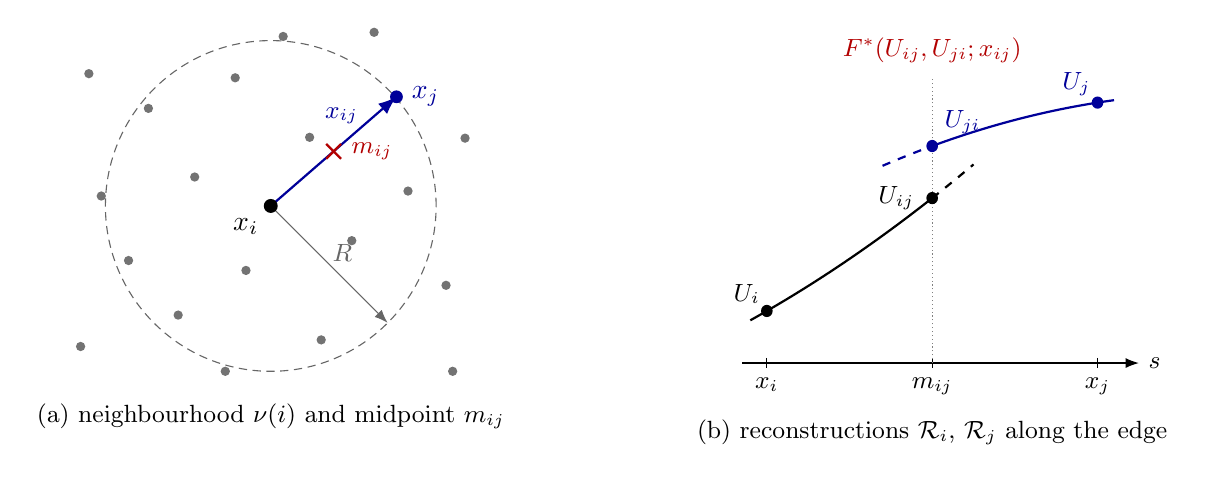
\begin{tikzpicture}[scale=1.05,>=Latex]
  % --- (a) stencil
  \begin{scope}
    \foreach \p in {(-2.05,0.12),(-1.48,1.18),(-1.12,-1.32),(-0.92,0.35),(-0.43,1.55),(-0.30,-0.78),(0.47,0.83),(0.61,-1.62),(0.98,-0.42),(1.52,1.32),(1.66,0.18),(2.12,-0.96),(-1.72,-0.66),(0.15,2.05),(-0.55,-2.0),(1.25,2.1),(2.35,0.82),(-2.2,1.6),(-2.3,-1.7),(2.2,-2.0)}
      \fill[black!55] \p circle (1.6pt);
    \draw[densely dashed,black!60] (0,0) circle (2.0);
    \draw[->,black!60] (0,0) -- (1.414,-1.414) node[midway,above right,inner sep=1pt] {\small $R$};
    \coordinate (I) at (0,0);
    \coordinate (J) at (1.52,1.32);
    \coordinate (M) at ($(I)!0.5!(J)$);
    \draw[thick,->,blue!60!black] (I) -- (J);
    \node[blue!60!black,above left,inner sep=1pt] at ($(I)!0.72!(J)$) {\small $x_{ij}$};
    \fill[blue!60!black] (J) circle (2.2pt) node[right=2pt] {$x_j$};
    \fill[black] (I) circle (2.4pt) node[below left=1pt] {$x_i$};
    \draw[red!70!black,thick] ($(M)+(-0.09,-0.09)$) -- ($(M)+(0.09,0.09)$) ($(M)+(-0.09,0.09)$) -- ($(M)+(0.09,-0.09)$);
    \node[red!70!black,right=3pt] at (M) {\small $m_{ij}$};
    \node at (0,-2.55) {\small (a) neighbourhood $\nb(i)$ and midpoint $m_{ij}$};
  \end{scope}
  % --- (b) 1D cut along the edge
  \begin{scope}[xshift=6.0cm,yshift=-1.9cm,yscale=1.05]
    \draw[->] (-0.3,0) -- (4.5,0) node[right] {\small $s$};
    \draw (0,0.06) -- (0,-0.06) node[below] {\small $x_i$};
    \draw (2,0.06) -- (2,-0.06) node[below] {\small $m_{ij}$};
    \draw (4,0.06) -- (4,-0.06) node[below] {\small $x_j$};
    \draw[densely dotted,black!50] (2,0) -- (2,3.3);
    \draw[thick,black] plot[domain=-0.2:2.0,samples=40] (\x,{0.6+0.55*\x+0.05*\x*\x});
    \draw[thick,black,dashed] plot[domain=2.0:2.5,samples=20] (\x,{0.6+0.55*\x+0.05*\x*\x});
    \draw[thick,blue!60!black] plot[domain=2.0:4.2,samples=40] (\x,{3.0-0.15*(4-\x)-0.05*(4-\x)*(4-\x)});
    \draw[thick,blue!60!black,dashed] plot[domain=1.4:2.0,samples=20] (\x,{3.0-0.15*(4-\x)-0.05*(4-\x)*(4-\x)});
    \fill[black] (0,0.6) circle (2pt) node[above left=-1pt] {\small $U_i$};
    \fill[blue!60!black] (4,3.0) circle (2pt) node[above left=-1pt] {\small $U_j$};
    \fill[black] (2,1.9) circle (2pt) node[left=3pt] {\small $U_{ij}$};
    \fill[blue!60!black] (2,2.5) circle (2pt) node[above right=1pt] {\small $U_{ji}$};
    \node[red!70!black] at (2,3.6) {\small $\Fs(U_{ij},U_{ji};x_{ij})$};
    \node at (2,-0.8) {\small (b) reconstructions $\mathcal{R}_i$, $\mathcal{R}_j$ along the edge};
  \end{scope}
\end{tikzpicture}
\caption{The meshfree MUSCL scheme. (a) Particle $i$, its neighbourhood $\nb(i)$ of radius $R$ and the midpoint $m_{ij}$ of the pair $(i,j)$. (b) The reconstructions of $i$ and $j$, evaluated at $m_{ij}$, define a Riemann problem whose numerical flux enters the updates of both particles.}\label{fig:stencil}
\end{figure}

\subsection{Reconstruction}\label{sec:recfit}

We use Taylor monomials $y^\alpha/\alpha!$ with $1\le|\alpha|\le r$, collected in the vector $p_r(y)$. The reconstruction of degree $r=k_i-1$ at particle $i$ fits the state differences in a weighted least-squares sense,
\begin{equation}\label{eq:recfit}
\min_{A}\ \sum_{j\in\nb(i)} w_{ij}\,\big| A^{\mathsf T}p_r(x_{ij}) - (U_j - U_i)\big|^2 ,\qquad
\mathcal{R}_i(y) = U_i + A_i^{\mathsf T}p_r(y),
\end{equation}
component by component in conservative variables. The fit passes through the particle value, $\mathcal{R}_i(0)=U_i$, and reproduces polynomials of degree $r$ exactly. For $k_i=1$ the reconstruction is constant. The fits are formulated in the scaled variable $y/h$, and nearly singular moment matrices are regularized by a small multiple of their trace. On a fixed cloud the inverse moment matrices are computed once and reused. A particle whose order is lowered by MOOD refits its reconstruction with the lower degree, and a lower order at a single interface truncates the existing polynomial (\cref{sec:epd}). The truncated polynomial is not the least-squares fit of the lower degree: its low-order coefficients are those of the higher-degree fit, which near a discontinuity can carry its oscillations. The first MOOD scheme also lowered the degree by truncating the reconstruction \cite{Clain2011}; for maximal degrees above two this was later found to behave undesirably at discontinuities \cite[Remark~4]{Diot2012}, and subsequent MOOD schemes recompute the reconstruction with the lower degree \cite{Diot2013,Loubere2014}. At order one, the case that the positivity argument of \cref{sec:positivity} needs, the truncation is the constant $U_i$ and coincides with the refit; for intermediate interface orders a refit per interface would be more robust but more expensive, and we have not compared the two. Ghost particles carry no reconstruction.

\subsection{Derivative operator}\label{sec:divfit}

The derivative weights come from a second fit of degree $q$, now \emph{with} a constant term and over the neighbours only. If $a_0+a^{\mathsf T}p_q(y)$ is the weighted least-squares fit of data $g_j$ at the offsets $x_{ij}$, the weights $c^{(d)}_{ij}$ are defined by $a_d=\sum_jc^{(d)}_{ij}g_j$, the coefficient of the linear monomial $y_d$; explicitly
\begin{equation}\label{eq:cij}
c^{(d)}_{ij} = w_{ij}\; e_{1+d}^{\mathsf T}\,\Ntil_i^{-1}\,\ptil_q(x_{ij}),\qquad
\Ntil_i=\sum_{j\in\nb(i)} w_{ij}\,\ptil_q(x_{ij})\,\ptil_q(x_{ij})^{\mathsf T},\qquad \ptil_q=(1,p_q).
\end{equation}
These weights differentiate polynomials of degree $q$ exactly, they scale like $1/h$, and, because constant data are absorbed by the intercept $a_0$, they sum to zero, $\sum_jc_{ij}=0$. This last property is what makes the update \eqref{eq:scheme} depend on fluxes only. A fit forced through the particle value, like the reconstruction, would not have it on irregular stencils: on the perturbed clouds of \cref{sec:experiments} its row sums amount to about $4\%$ of $\sum_j|c_{ij}|$ on average and up to $19\%$ (\cref{tab:stencils}).

\subsection{Choice of the derivative degree}\label{sec:parity}

On a centrally symmetric stencil, such as a lattice, every neighbour $j$ has a mirror neighbour $j'$ with $x_{ij'}=-x_{ij}$, and the fit does not mix even and odd monomials. Two consequences follow. First, mirrored neighbours get opposite weights, $c_{ij'}=-c_{ij}$, as in a central difference. Second, if $q$ is odd, the first monomial the fit cannot represent, of degree $q+1$, is even and does not affect the derivative, so the derivative is exact one degree beyond $q$. For even $q$ the first missing monomial is odd and leaks into the derivative. For a smooth function the derivative error is therefore $O(h^{q+1})$ for odd $q$ on symmetric stencils and $O(h^q)$ otherwise: an odd degree is worth one order. For design order $k$ we therefore use the smallest odd degree not below $k-1$,
\begin{equation}\label{eq:qk}
\qdiv(k) = 2\lceil k/2\rceil - 1,
\end{equation}
which equals $k-1$ for even $k$ and $k$ for odd $k$ (\cref{tab:degrees}).

\begin{table}[!htbp]
\centering
\caption{Polynomial degrees of the scheme of design order $k$ and the number of unknowns of the fits in two dimensions.}\label{tab:degrees}
\begin{tabular}{lcccccc}
\toprule
design order $k$ & 1 & 2 & 3 & 4 & 5 & 6\\
\midrule
reconstruction degree $k-1$ & 0 & 1 & 2 & 3 & 4 & 5\\
derivative degree $\qdiv(k)$ & 1 & 1 & 3 & 3 & 5 & 5\\
unknowns of the reconstruction fit ($D=2$) & -- & 2 & 5 & 9 & 14 & 20\\
unknowns of the derivative fit ($D=2$) & 3 & 3 & 10 & 10 & 21 & 21\\
\bottomrule
\end{tabular}
\end{table}

Two safeguards keep the fits well posed. The increase from degree $k-1$ to $k$ is only used if the neighbourhood contains at least $1.5$ times as many particles as the fit has unknowns, because nearly square least-squares systems are fragile; in three dimensions it is only applied up to degree three. And every fit lowers its degree until there are at least as many neighbours as unknowns. With $\kappa=2.5$ the two-dimensional stencils support the degrees of \cref{tab:degrees} up to $k=4$. In one dimension $\kappa=2.5$ gives only four neighbours, so $k=3$ falls back to derivative degree two, and on perturbed clouds $k=5$ needs about $\kappa\ge5.5$ in one and $\kappa\ge3.5$ in two dimensions (on lattices $\kappa=5$ and $\kappa\approx3.2$ suffice).

The derivative degree can be chosen in two ways. In the \emph{coupled} mode it follows the current order, $q_i=\qdiv(k_i)$. In the \emph{frozen} mode it is fixed, $q_i=\qdiv(k_{\mathrm{div}})$ for a prescribed $k_{\mathrm{div}}\le K$, independently of what MOOD does. Both coincide if no order is lowered and $\qdiv(k_{\mathrm{div}})=\qdiv(K)$, in particular for $K\le2$; for example, $k_{\mathrm{div}}=2$ with $K=4$ uses degree-one weights even where no order is lowered. The frozen mode with the aligned flux of the next subsection is our recommended choice. The coupled mode was the original design and is included for comparison: a lowered particle next to a high-order one forms a pair with two different derivative degrees, and such pairs turn out to be the main source of conservation errors (\cref{sec:conservation,sec:mass}).

\subsection{Interface fluxes}\label{sec:fluxes}

With interface orders $\ord ij\le k_i$ prescribed by MOOD (\cref{sec:epd}; without MOOD $\ord ij=K$), the interface states are the reconstructions evaluated at the midpoint,
\begin{equation}\label{eq:states}
U_{ij} = \mathcal{R}^{[\ord ij]}_i\big(\tfrac12 x_{ij}\big),\qquad U_{ji}=\mathcal{R}^{[\ord ji]}_j\big(-\tfrac12 x_{ij}\big),
\end{equation}
where $\mathcal{R}^{[r]}$ denotes the reconstruction truncated to degree $r-1$, and $U_{ji}=U_j$ for ghost neighbours. Since the derivative operator differentiates every coordinate flux separately, we solve a Riemann problem per coordinate direction with the Rusanov (local Lax--Friedrichs) flux \cite{Toro2009},
\begin{equation}\label{eq:rusanov}
\Fs_{ij,d} = \tfrac12\big(F_d(U_{ij})+F_d(U_{ji})\big) - \tfrac12\,s_{ij,d}\,\sigma_{ij,d}\,\big(U_{ji}-U_{ij}\big),\qquad
s_{ij,d} = \max\{\lambda_d(U_{ij}),\lambda_d(U_{ji})\}.
\end{equation}
The orientation $\sigma_{ij,d}=\pm1$ decides which of the two states counts as the left one. On a mesh the natural choice is \emph{geometric}, $\sigma_{ij,d}=\sgn(x_{ij,d})$. On a point cloud this choice can fail. Inserted into \eqref{eq:scheme}, the dissipation of neighbour $j$ enters the update of particle $i$ with the coefficient $s_{ij,d}\,\sigma_{ij,d}c^{(d)}_{ij}$, which should be non-negative so that the term pulls $U_i$ towards its neighbours. With the geometric orientation it is negative wherever a weight has the opposite sign of its offset. That happens for the outer neighbours of every derivative fit of degree three or higher, just as in the fourth-order central difference $(f_{-2}-8f_{-1}+8f_1-f_2)/(12h)$, and for a few small weights of degree-one fits on perturbed clouds (\cref{tab:stencils}). There the dissipation acts as anti-dissipation.

We therefore use the \emph{aligned} orientation $\sigma_{ij,d}=\sgn(c^{(d)}_{ij})$ on every edge where at least one of the two particles has an order below $K$, and, when the aligned flux is selected, on all edges of the first-order scheme $K=1$ (the baseline RK2MUSCL1 of \cref{sec:experiments} uses the geometric orientation instead); elsewhere we keep the geometric orientation. The first-order scheme needs it even with degree-one weights: with the geometric orientation, $3.2\%$ of its dissipation coefficients are negative on a perturbed cloud (\cref{tab:stencils}), the most negative ones about half as large as the mean coefficient. All dissipation coefficients then become $s_{ij,d}|c^{(d)}_{ij}|\ge0$ near troubled regions, which is exactly what the positivity of the first-order scheme needs (\cref{sec:positivity}). In a high-order scheme, where no order is lowered, nothing changes, so its accuracy is unaffected. Each particle uses the sign of its own weight, taken from the derivative weights it actually multiplies the fluxes with, i.e.\ from the fit of its current degree $q_i$; a sign taken from a fit of another degree would guarantee nothing. On the few pairs where $c^{(d)}_{ij}$ and $c^{(d)}_{ji}$ have the same sign ($5\%$ of the pairs and directions for degree one and $19\%$ for degree three on the perturbed clouds of \cref{tab:stencils}, carrying $0.4\%$ and $4.7\%$ of the weight), the two particles therefore compute slightly different fluxes; on a lattice this cannot happen. For scalar equations the dissipation coefficient may instead be the Rankine--Hugoniot speed, which gives the upwind flux.

\subsection{Accuracy}\label{sec:consistency}

For a linear problem with a polynomial solution of degree $k-1$, every step of the scheme is exact: both reconstructions reproduce the solution, the two interface states agree, the Riemann problem has no jump, and the midpoint fluxes, again a polynomial of degree $k-1$, are differentiated exactly. This holds on arbitrary point clouds as long as $q_i\ge k-1$, and it is the meshfree analogue of a $(k-1)$-exact reconstruction in FV methods, which yields schemes of order $k$ \cite{BarthFrederickson1990}. This is the sense in which we call $k$ the design order.

For smooth solutions the reconstruction errors at the midpoints are of size $O(h^k)$, and the weights, of size $O(h^{-1})$, would amplify them to a truncation error of $O(h^{k-1})$. On a lattice, however, the leading reconstruction errors seen from the two ends of an edge are mirror images of each other, the resulting flux error is an even function of the offset, and the odd derivative weights cancel it. A Taylor expansion then gives the truncation error
\begin{equation}\label{eq:lattice}
\Lop_i(U) + \nabla\cdot F(U)(x_i) = O\big(h^{\min(k,\,q+1)}\big)
\end{equation}
on lattices with odd $q$, i.e.\ order $k$ for $q=\qdiv(k)$. With the even degree $q=k-1$ for odd $k$ the scheme would only be of order $k-1$, which is a second reason for \eqref{eq:qk}. The estimate also shows that the frozen mode with a low derivative degree, for instance $k_{\mathrm{div}}=2$ with $K=4$, is formally of order $\qdiv(k_{\mathrm{div}})+1$ only, although its reconstructions are of higher degree. On irregular clouds the cancellation is not exact; for kernel-based particle approximations such as SPH, truncation errors on disordered point sets may even stagnate or grow under refinement \cite{Quinlan2006}, while observed errors still converge at the design order, as for FV schemes on irregular grids \cite{Diskin2010}. The convergence study of \cref{sec:smooth} measures the actual rates.

\subsection{Conservation}\label{sec:conservation}

Summing the volume-weighted updates \eqref{eq:scheme} over all interior particles, every interior pair appears twice, once from each side, and one obtains
\begin{equation}\label{eq:balance}
\begin{aligned}
\frac{\dd}{\dd t}\sum_{i\in I}V_iU_i
={}& -2\sum_{i\in I}\ \sum_{j\in\nb(i)\setminus I} V_i\,c_{ij}\cdot\Fs_{ij}\\
&-\sum_{\substack{\{i,j\}\subset I\\ j\in\nb(i)}}\ \sum_{d=1}^D\Big[d_{ij,d}\,\big(F_d(U_{ij})+F_d(U_{ji})\big)-s_{ij,d}\,e_{ij,d}\,\big(U_{ji}-U_{ij}\big)\Big]
\end{aligned}
\end{equation}
with the pair defects $d_{ij,d}=V_ic^{(d)}_{ij}+V_jc^{(d)}_{ji}$ and $e_{ij,d}=V_i\sigma_{ij,d}c^{(d)}_{ij}-V_j\sigma_{ji,d}c^{(d)}_{ji}$, where $|e_{ij,d}|\le|d_{ij,d}|$ for both orientations, except on geometric edges with $x_{ij,d}=0$, on which the implementation sets $\sigma_{ij,d}=\sigma_{ji,d}=-1$ and the bound can fail. The first sum plays the role of the boundary fluxes. The second sum vanishes, and the scheme is conservative, if the generalized face vectors $S_{ij}=2V_ic_{ij}$ are antisymmetric, $S_{ij}=-S_{ji}$, just as the normals of a mesh face seen from its two cells, and if on the edges with $x_{ij,d}=0$ either $c^{(d)}_{ij}=0$ or $\sigma_{ji,d}=-\sigma_{ij,d}$; we do not claim the converse. The update can always be written as $V_i\,\dd U_i/\dd t=-\sum_jS_{ij}\cdot\Fs_{ij}$ by the definition of $S_{ij}$ and the closure $\sum_jS_{ij}=0$ from the zero row sums; with antisymmetric $S_{ij}$ it is a conservative FV-type update. Meshless coefficients with both properties can be constructed \cite{Chiu2011,Chiu2012}; other methods enforce the closure alone \cite{Huh2018} or approximately conservative fluxes over closed local cells \cite{Suchde2017,SuchdeThesis2018}; we do not apply such a correction here.

The MLS weights are antisymmetric on lattices with equal volumes, but not on irregular clouds. \Cref{tab:stencils} in \cref{app:stencils} quantifies the relative pair defect $\sum|V_ic_{ij}+V_jc_{ji}|/\sum(|V_ic_{ij}|+|V_jc_{ji}|)$ on the clouds of \cref{sec:experiments}: about $5\%$ for degree one and $17\%$ for degree three, and about $73\%$ for pairs whose two particles use different degrees, even on an unperturbed lattice. In the coupled mode with $K\ge3$, MOOD creates such mixed pairs at the boundaries of every lowered region, which is where its conservation defect concentrates. The frozen mode avoids them. The remaining defects of equal-degree pairs belong to the fixed stencils and do not depend on MOOD; their effect decreases under refinement, also at moving shocks (\cref{sec:mass}).

% ===========================================================================
\section{Treatment of discontinuities}\label{sec:mood}
% ===========================================================================

\subsection{A priori slope limiters}\label{sec:limiters}

Slope limiters scale the reconstruction coefficients before they are used. For the multidimensional limiters of Barth--Jespersen (BJ) \cite{BarthJespersen1989} and Venkatakrishnan (VK) \cite{Venkatakrishnan1995}, the increments $\Delta_{ij}=\mathcal{R}_i(\tfrac12x_{ij})-U_i$ at the midpoints are compared, component by component, with the distance to the extrema $U^{\max}_i$, $U^{\min}_i$ over $\cnb(i)$. With the ratio $r_{ij}=(U^{\max}_i-U_i)/\Delta_{ij}$ for $\Delta_{ij}>0$ (and with $U^{\min}_i$ for $\Delta_{ij}<0$), the limiter factor is $\phi_i=\min\{1,\min_j\phi(r_{ij})\}$ with
\begin{equation}
\phi_{\mathrm{BJ}}(r)=\min\{1,r\},\qquad \phi_{\mathrm{VK}}(r)=\frac{r^2+2r}{r^2+r+2}.
\end{equation}
The factor is applied to all coefficients (\emph{hard} mode), which keeps all midpoint values within the local bounds, or to the gradient only (\emph{soft} mode). In one dimension the minmod and superbee limiters \cite{Roe1985,Sweby1984} are also available. Limiters and MOOD can be combined.

\subsection{MOOD detection}\label{sec:criteria}

MOOD works with the per-particle orders $k_i$, which are reset to $K$ at the beginning of every time step. A candidate state $U^*_i$ is flagged if one of the following criteria fails.
\begin{itemize}
\item \emph{Physical admissibility detection (PAD)} \cite{Diot2012,Diot2013}: $U^*_i$ must be finite with positive density and pressure.
\item \emph{Relaxed discrete maximum principle (DMP)} \cite{Clain2011,Diot2013,Dumbser2014}: with the extrema $U^{\max}_{i,m}$, $U^{\min}_{i,m}$ of component $m$ over $\cnb(i)$ of the previous state, the candidate fails if for some $m$
\begin{equation}\label{eq:dmp}
U^{\max}_{i,m}-U^{\min}_{i,m}\ge\delta^3\quad\text{and}\quad U^*_{i,m}\notin\big[U^{\min}_{i,m}-\delta,\ U^{\max}_{i,m}+\delta\big],
\end{equation}
with $\delta=\delta_0\prod_dh_d$, where $h_d$ is the nominal spacing in direction $d$. The first condition ignores flat regions, and the relaxation absorbs small overshoots. Since $\delta$ scales with $h^D$, it becomes small on fine clouds: for the Riemann problem, the double Mach reflection and the step of \cref{sec:experiments} it lies between $1.6\cdot10^{-10}$ and $1.1\cdot10^{-9}$, below the resolution of single precision, so that there the relaxation and the flat-region guard are inactive and the plateau test below takes over their role.
\item \emph{Plateau test.} A component that violates the DMP is nevertheless accepted if it varies across the stencil by less than a fraction $\pi_0$ of its global range, $U^{\max}_{i,m}-U^{\min}_{i,m}<\pi_0\,\big(\max_lU_{l,m}-\min_lU_{l,m}\big)$, with the global extrema over all particles of the previous state. Such a component carries no structure at the scale of the stencil, and what violates the DMP there is the truncation error of the update, for instance the density in the far field of a vortex, which is driven by the divergence of the momentum. The test needs no curvature and therefore also applies below order three. We use $\pi_0=10^{-3}$. Overshoots are thus accepted only where the variation across the stencil is below $10^{-3}$ of the global range, which also means that features of smaller amplitude are not limited.
\item \emph{Smooth-extremum detection (u2)}, adapted from the criterion called u2 in \cite{Diot2012,Diot2013}: for $K\ge3$ and $k_i\ge3$, a component $m$ that violates the DMP and is not a plateau is nevertheless accepted if, in every direction $d$, the second-derivative coefficients $X_l$ of the reconstructions of the previous state indicate a smooth extremum. The curvatures are measured by the variation $X_lh^2$ they cause over one particle spacing, so that they can be compared with $\delta$ in the units of the state. The component is accepted if the curvature is negligible, $\max_l|X_l|\,h^2<\delta$, or if it has one sign over the whole stencil and comparable magnitudes among the nearest neighbours,
\begin{equation}\label{eq:u2}
\big(\min_{l\in\cnb(i)}X_l\,h^2\big)\big(\max_{l\in\cnb(i)}X_l\,h^2\big)>-\delta^2\qquad\text{and}\qquad\min_{l\in\nb_{1.5}(i)}|X_l|\ge\frac12\max_{l\in\nb_{1.5}(i)}|X_l|,
\end{equation}
where $\nb_{1.5}(i)$ contains $i$ and its neighbours within $1.5h$. The magnitudes are compared only over the nearest neighbours, which play the role of the face neighbours that the test of \cite{Diot2012} uses on meshes: over a whole meshfree stencil of radius $2.5h$ the curvature of a smooth solution changes by more than a factor two wherever it decays on a few spacings. The magnitude test is still needed, because next to a jump the curvature collapses from large values to zero between neighbours, which the sign test does not see. Only the components that violate the DMP are tested. For $K\le2$ no curvature is available, and smooth extrema that are not plateaus are clipped.
\end{itemize}
A flagged particle with $k_i>1$ lowers its order by one. A flagged particle at order one keeps its candidate, so the robustness of the method rests on the first-order scheme.

\subsection{A positive first-order fallback}\label{sec:positivity}

At order one the interface states are constant, $U_{ij}=U_i$ and $U_{ji}=U_j$. Because the weights sum to zero, all terms with $F(U_i)$ drop out of \eqref{eq:scheme}, and with the aligned orientation, where $\sigma_{ij,d}c^{(d)}_{ij}=|c^{(d)}_{ij}|$, a forward Euler step can be rearranged into
\begin{equation}\label{eq:convex}
U_i+\Delta t\,\Lop_i(U)=\Big(1-\Delta t\sum_{j,d}s_{ij,d}|c^{(d)}_{ij}|\Big)U_i+\sum_{j,d}\Delta t\,s_{ij,d}|c^{(d)}_{ij}|\Big(U_j-\sigma_{ij,d}\frac{F_d(U_j)}{s_{ij,d}}\Big).
\end{equation}
For the Euler equations, the states $U_j-\sigma F_d(U_j)/s$ in the last sum have positive density and pressure whenever $s\ge|u_d|+c$, a classical property of Lax--Friedrichs schemes \cite{PerthameShu1996,ZhangShu2010}. Under the meshfree CFL condition
\begin{equation}\label{eq:cflpos}
\Delta t\sum_{j\in\nb(i)}\sum_{d=1}^Ds_{ij,d}\,|c^{(d)}_{ij}|\le1,
\end{equation}
all coefficients in \eqref{eq:convex} are non-negative and sum to one, so the new state is a convex combination of admissible states and is itself admissible. This holds for derivative weights of any degree. For scalar conservation laws the same rearrangement shows that the first-order update stays between the local minimum and maximum if $2\Delta t\sum_{j,d}s_{ij,d}|c^{(d)}_{ij}|\le1$ and $s_{ij,d}\ge|F_d'|$ on the interval between $U_i$ and $U_j$.

With the geometric orientation the argument requires $\sgn c^{(d)}_{ij}=\sgn x_{ij,d}$ for all weights, which fails for $40\%$ of the degree-three weights on lattices and for $44\%$ on perturbed clouds. A Monte Carlo test with $2\times10^4$ random first-order updates of random admissible Euler states at the limit of \eqref{eq:cflpos} on a perturbed $48\times48$ cloud shows the consequence: with degree-three weights, about $9\%$ of the updates with the geometric orientation produce negative density or pressure, and none with the aligned orientation; with degree-one weights all updates are admissible for both. The price of the aligned orientation is more dissipation at lowered particles; with degree-three weights the dissipation coefficient is about $2.7$ times that of degree-one weights. Since the orientation is read from the weights in use, the argument holds in the frozen and in the coupled mode; the coupled mode, however, creates pairs of different derivative degrees, which are not conservative (\cref{sec:conservation,sec:mass}).

\subsection{Interface orders}\label{sec:epd}

When MOOD lowers some orders, the two sides of an edge may have different orders, and a rule has to decide which polynomial degree each side uses at the interface. In FV MOOD the degree at a face is typically the minimum of the two adjacent cells \cite{Clain2011,Diot2012}. We consider three such \emph{edge polynomial degree} (EPD) rules for the edges of the neighbour graph:
\begin{equation}\label{eq:epd}
\begin{aligned}
&\text{EPD0:}&\ \ \ord ij&=k_i,\\
&\text{EPD1:}&\ \ \ord ij&=\ord ji=\min\{k_i,k_j\},\\
&\text{EPD2:}&\ \ \ord ij&=\ord ji=\min\{k_l: l\in\cnb(i)\cup\cnb(j)\}.
\end{aligned}
\end{equation}
EPD1 is the minimum rule of FV MOOD; EPD0 and EPD2 are, to our knowledge, new. In contrast to the meshless MOOD of \cite{Willems2025}, which replaces a flagged update by the first-order scheme in one step, the orders here are lowered one by one. \Cref{fig:epd} illustrates the rules for a single particle at order one. From EPD0 to EPD2 the transition between high and low order becomes wider and smoother.

\begin{figure}[!htbp]
\centering
% generated by scripts/make_epd_figure_light.py
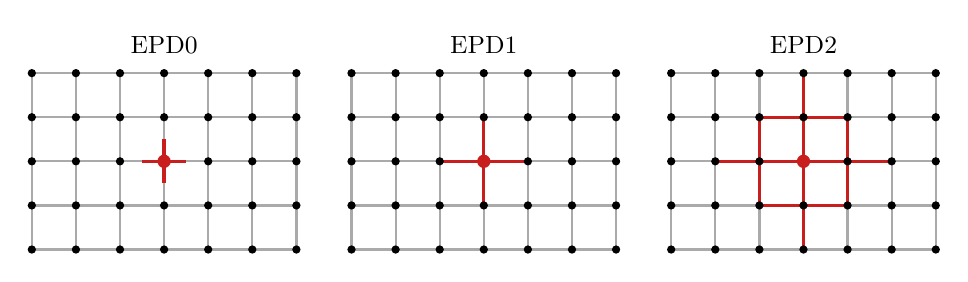
\begin{tikzpicture}
\draw[highc,thick] (0.000,0.000) -- (0.000,0.280);
\draw[highc,thick] (0.000,0.560) -- (0.000,0.280);
\draw[highc,thick] (0.000,0.000) -- (0.280,0.000);
\draw[highc,thick] (0.560,0.000) -- (0.280,0.000);
\draw[highc,thick] (0.000,0.560) -- (0.000,0.840);
\draw[highc,thick] (0.000,1.120) -- (0.000,0.840);
\draw[highc,thick] (0.000,0.560) -- (0.280,0.560);
\draw[highc,thick] (0.560,0.560) -- (0.280,0.560);
\draw[highc,thick] (0.000,1.120) -- (0.000,1.400);
\draw[highc,thick] (0.000,1.680) -- (0.000,1.400);
\draw[highc,thick] (0.000,1.120) -- (0.280,1.120);
\draw[highc,thick] (0.560,1.120) -- (0.280,1.120);
\draw[highc,thick] (0.000,1.680) -- (0.000,1.960);
\draw[highc,thick] (0.000,2.240) -- (0.000,1.960);
\draw[highc,thick] (0.000,1.680) -- (0.280,1.680);
\draw[highc,thick] (0.560,1.680) -- (0.280,1.680);
\draw[highc,thick] (0.000,2.240) -- (0.280,2.240);
\draw[highc,thick] (0.560,2.240) -- (0.280,2.240);
\draw[highc,thick] (0.560,0.000) -- (0.560,0.280);
\draw[highc,thick] (0.560,0.560) -- (0.560,0.280);
\draw[highc,thick] (0.560,0.000) -- (0.840,0.000);
\draw[highc,thick] (1.120,0.000) -- (0.840,0.000);
\draw[highc,thick] (0.560,0.560) -- (0.560,0.840);
\draw[highc,thick] (0.560,1.120) -- (0.560,0.840);
\draw[highc,thick] (0.560,0.560) -- (0.840,0.560);
\draw[highc,thick] (1.120,0.560) -- (0.840,0.560);
\draw[highc,thick] (0.560,1.120) -- (0.560,1.400);
\draw[highc,thick] (0.560,1.680) -- (0.560,1.400);
\draw[highc,thick] (0.560,1.120) -- (0.840,1.120);
\draw[highc,thick] (1.120,1.120) -- (0.840,1.120);
\draw[highc,thick] (0.560,1.680) -- (0.560,1.960);
\draw[highc,thick] (0.560,2.240) -- (0.560,1.960);
\draw[highc,thick] (0.560,1.680) -- (0.840,1.680);
\draw[highc,thick] (1.120,1.680) -- (0.840,1.680);
\draw[highc,thick] (0.560,2.240) -- (0.840,2.240);
\draw[highc,thick] (1.120,2.240) -- (0.840,2.240);
\draw[highc,thick] (1.120,0.000) -- (1.120,0.280);
\draw[highc,thick] (1.120,0.560) -- (1.120,0.280);
\draw[highc,thick] (1.120,0.000) -- (1.400,0.000);
\draw[highc,thick] (1.680,0.000) -- (1.400,0.000);
\draw[highc,thick] (1.120,0.560) -- (1.120,0.840);
\draw[highc,thick] (1.120,1.120) -- (1.120,0.840);
\draw[highc,thick] (1.120,0.560) -- (1.400,0.560);
\draw[highc,thick] (1.680,0.560) -- (1.400,0.560);
\draw[highc,thick] (1.120,1.120) -- (1.120,1.400);
\draw[highc,thick] (1.120,1.680) -- (1.120,1.400);
\draw[highc,thick] (1.120,1.120) -- (1.400,1.120);
\draw[lowc,very thick] (1.680,1.120) -- (1.400,1.120);
\draw[highc,thick] (1.120,1.680) -- (1.120,1.960);
\draw[highc,thick] (1.120,2.240) -- (1.120,1.960);
\draw[highc,thick] (1.120,1.680) -- (1.400,1.680);
\draw[highc,thick] (1.680,1.680) -- (1.400,1.680);
\draw[highc,thick] (1.120,2.240) -- (1.400,2.240);
\draw[highc,thick] (1.680,2.240) -- (1.400,2.240);
\draw[highc,thick] (1.680,0.000) -- (1.680,0.280);
\draw[highc,thick] (1.680,0.560) -- (1.680,0.280);
\draw[highc,thick] (1.680,0.000) -- (1.960,0.000);
\draw[highc,thick] (2.240,0.000) -- (1.960,0.000);
\draw[highc,thick] (1.680,0.560) -- (1.680,0.840);
\draw[lowc,very thick] (1.680,1.120) -- (1.680,0.840);
\draw[highc,thick] (1.680,0.560) -- (1.960,0.560);
\draw[highc,thick] (2.240,0.560) -- (1.960,0.560);
\draw[lowc,very thick] (1.680,1.120) -- (1.680,1.400);
\draw[highc,thick] (1.680,1.680) -- (1.680,1.400);
\draw[lowc,very thick] (1.680,1.120) -- (1.960,1.120);
\draw[highc,thick] (2.240,1.120) -- (1.960,1.120);
\draw[highc,thick] (1.680,1.680) -- (1.680,1.960);
\draw[highc,thick] (1.680,2.240) -- (1.680,1.960);
\draw[highc,thick] (1.680,1.680) -- (1.960,1.680);
\draw[highc,thick] (2.240,1.680) -- (1.960,1.680);
\draw[highc,thick] (1.680,2.240) -- (1.960,2.240);
\draw[highc,thick] (2.240,2.240) -- (1.960,2.240);
\draw[highc,thick] (2.240,0.000) -- (2.240,0.280);
\draw[highc,thick] (2.240,0.560) -- (2.240,0.280);
\draw[highc,thick] (2.240,0.000) -- (2.520,0.000);
\draw[highc,thick] (2.800,0.000) -- (2.520,0.000);
\draw[highc,thick] (2.240,0.560) -- (2.240,0.840);
\draw[highc,thick] (2.240,1.120) -- (2.240,0.840);
\draw[highc,thick] (2.240,0.560) -- (2.520,0.560);
\draw[highc,thick] (2.800,0.560) -- (2.520,0.560);
\draw[highc,thick] (2.240,1.120) -- (2.240,1.400);
\draw[highc,thick] (2.240,1.680) -- (2.240,1.400);
\draw[highc,thick] (2.240,1.120) -- (2.520,1.120);
\draw[highc,thick] (2.800,1.120) -- (2.520,1.120);
\draw[highc,thick] (2.240,1.680) -- (2.240,1.960);
\draw[highc,thick] (2.240,2.240) -- (2.240,1.960);
\draw[highc,thick] (2.240,1.680) -- (2.520,1.680);
\draw[highc,thick] (2.800,1.680) -- (2.520,1.680);
\draw[highc,thick] (2.240,2.240) -- (2.520,2.240);
\draw[highc,thick] (2.800,2.240) -- (2.520,2.240);
\draw[highc,thick] (2.800,0.000) -- (2.800,0.280);
\draw[highc,thick] (2.800,0.560) -- (2.800,0.280);
\draw[highc,thick] (2.800,0.000) -- (3.080,0.000);
\draw[highc,thick] (3.360,0.000) -- (3.080,0.000);
\draw[highc,thick] (2.800,0.560) -- (2.800,0.840);
\draw[highc,thick] (2.800,1.120) -- (2.800,0.840);
\draw[highc,thick] (2.800,0.560) -- (3.080,0.560);
\draw[highc,thick] (3.360,0.560) -- (3.080,0.560);
\draw[highc,thick] (2.800,1.120) -- (2.800,1.400);
\draw[highc,thick] (2.800,1.680) -- (2.800,1.400);
\draw[highc,thick] (2.800,1.120) -- (3.080,1.120);
\draw[highc,thick] (3.360,1.120) -- (3.080,1.120);
\draw[highc,thick] (2.800,1.680) -- (2.800,1.960);
\draw[highc,thick] (2.800,2.240) -- (2.800,1.960);
\draw[highc,thick] (2.800,1.680) -- (3.080,1.680);
\draw[highc,thick] (3.360,1.680) -- (3.080,1.680);
\draw[highc,thick] (2.800,2.240) -- (3.080,2.240);
\draw[highc,thick] (3.360,2.240) -- (3.080,2.240);
\draw[highc,thick] (3.360,0.000) -- (3.360,0.280);
\draw[highc,thick] (3.360,0.560) -- (3.360,0.280);
\draw[highc,thick] (3.360,0.560) -- (3.360,0.840);
\draw[highc,thick] (3.360,1.120) -- (3.360,0.840);
\draw[highc,thick] (3.360,1.120) -- (3.360,1.400);
\draw[highc,thick] (3.360,1.680) -- (3.360,1.400);
\draw[highc,thick] (3.360,1.680) -- (3.360,1.960);
\draw[highc,thick] (3.360,2.240) -- (3.360,1.960);
\fill[black] (0.000,0.000) circle (1.5pt);
\fill[black] (0.000,0.560) circle (1.5pt);
\fill[black] (0.000,1.120) circle (1.5pt);
\fill[black] (0.000,1.680) circle (1.5pt);
\fill[black] (0.000,2.240) circle (1.5pt);
\fill[black] (0.560,0.000) circle (1.5pt);
\fill[black] (0.560,0.560) circle (1.5pt);
\fill[black] (0.560,1.120) circle (1.5pt);
\fill[black] (0.560,1.680) circle (1.5pt);
\fill[black] (0.560,2.240) circle (1.5pt);
\fill[black] (1.120,0.000) circle (1.5pt);
\fill[black] (1.120,0.560) circle (1.5pt);
\fill[black] (1.120,1.120) circle (1.5pt);
\fill[black] (1.120,1.680) circle (1.5pt);
\fill[black] (1.120,2.240) circle (1.5pt);
\fill[black] (1.680,0.000) circle (1.5pt);
\fill[black] (1.680,0.560) circle (1.5pt);
\fill[lowc] (1.680,1.120) circle (2.4pt);
\fill[black] (1.680,1.680) circle (1.5pt);
\fill[black] (1.680,2.240) circle (1.5pt);
\fill[black] (2.240,0.000) circle (1.5pt);
\fill[black] (2.240,0.560) circle (1.5pt);
\fill[black] (2.240,1.120) circle (1.5pt);
\fill[black] (2.240,1.680) circle (1.5pt);
\fill[black] (2.240,2.240) circle (1.5pt);
\fill[black] (2.800,0.000) circle (1.5pt);
\fill[black] (2.800,0.560) circle (1.5pt);
\fill[black] (2.800,1.120) circle (1.5pt);
\fill[black] (2.800,1.680) circle (1.5pt);
\fill[black] (2.800,2.240) circle (1.5pt);
\fill[black] (3.360,0.000) circle (1.5pt);
\fill[black] (3.360,0.560) circle (1.5pt);
\fill[black] (3.360,1.120) circle (1.5pt);
\fill[black] (3.360,1.680) circle (1.5pt);
\fill[black] (3.360,2.240) circle (1.5pt);
\node[anchor=south] at (1.680,2.360) {\small EPD0};
\draw[highc,thick] (4.060,0.000) -- (4.060,0.280);
\draw[highc,thick] (4.060,0.560) -- (4.060,0.280);
\draw[highc,thick] (4.060,0.000) -- (4.340,0.000);
\draw[highc,thick] (4.620,0.000) -- (4.340,0.000);
\draw[highc,thick] (4.060,0.560) -- (4.060,0.840);
\draw[highc,thick] (4.060,1.120) -- (4.060,0.840);
\draw[highc,thick] (4.060,0.560) -- (4.340,0.560);
\draw[highc,thick] (4.620,0.560) -- (4.340,0.560);
\draw[highc,thick] (4.060,1.120) -- (4.060,1.400);
\draw[highc,thick] (4.060,1.680) -- (4.060,1.400);
\draw[highc,thick] (4.060,1.120) -- (4.340,1.120);
\draw[highc,thick] (4.620,1.120) -- (4.340,1.120);
\draw[highc,thick] (4.060,1.680) -- (4.060,1.960);
\draw[highc,thick] (4.060,2.240) -- (4.060,1.960);
\draw[highc,thick] (4.060,1.680) -- (4.340,1.680);
\draw[highc,thick] (4.620,1.680) -- (4.340,1.680);
\draw[highc,thick] (4.060,2.240) -- (4.340,2.240);
\draw[highc,thick] (4.620,2.240) -- (4.340,2.240);
\draw[highc,thick] (4.620,0.000) -- (4.620,0.280);
\draw[highc,thick] (4.620,0.560) -- (4.620,0.280);
\draw[highc,thick] (4.620,0.000) -- (4.900,0.000);
\draw[highc,thick] (5.180,0.000) -- (4.900,0.000);
\draw[highc,thick] (4.620,0.560) -- (4.620,0.840);
\draw[highc,thick] (4.620,1.120) -- (4.620,0.840);
\draw[highc,thick] (4.620,0.560) -- (4.900,0.560);
\draw[highc,thick] (5.180,0.560) -- (4.900,0.560);
\draw[highc,thick] (4.620,1.120) -- (4.620,1.400);
\draw[highc,thick] (4.620,1.680) -- (4.620,1.400);
\draw[highc,thick] (4.620,1.120) -- (4.900,1.120);
\draw[highc,thick] (5.180,1.120) -- (4.900,1.120);
\draw[highc,thick] (4.620,1.680) -- (4.620,1.960);
\draw[highc,thick] (4.620,2.240) -- (4.620,1.960);
\draw[highc,thick] (4.620,1.680) -- (4.900,1.680);
\draw[highc,thick] (5.180,1.680) -- (4.900,1.680);
\draw[highc,thick] (4.620,2.240) -- (4.900,2.240);
\draw[highc,thick] (5.180,2.240) -- (4.900,2.240);
\draw[highc,thick] (5.180,0.000) -- (5.180,0.280);
\draw[highc,thick] (5.180,0.560) -- (5.180,0.280);
\draw[highc,thick] (5.180,0.000) -- (5.460,0.000);
\draw[highc,thick] (5.740,0.000) -- (5.460,0.000);
\draw[highc,thick] (5.180,0.560) -- (5.180,0.840);
\draw[highc,thick] (5.180,1.120) -- (5.180,0.840);
\draw[highc,thick] (5.180,0.560) -- (5.460,0.560);
\draw[highc,thick] (5.740,0.560) -- (5.460,0.560);
\draw[highc,thick] (5.180,1.120) -- (5.180,1.400);
\draw[highc,thick] (5.180,1.680) -- (5.180,1.400);
\draw[lowc,very thick] (5.180,1.120) -- (5.460,1.120);
\draw[lowc,very thick] (5.740,1.120) -- (5.460,1.120);
\draw[highc,thick] (5.180,1.680) -- (5.180,1.960);
\draw[highc,thick] (5.180,2.240) -- (5.180,1.960);
\draw[highc,thick] (5.180,1.680) -- (5.460,1.680);
\draw[highc,thick] (5.740,1.680) -- (5.460,1.680);
\draw[highc,thick] (5.180,2.240) -- (5.460,2.240);
\draw[highc,thick] (5.740,2.240) -- (5.460,2.240);
\draw[highc,thick] (5.740,0.000) -- (5.740,0.280);
\draw[highc,thick] (5.740,0.560) -- (5.740,0.280);
\draw[highc,thick] (5.740,0.000) -- (6.020,0.000);
\draw[highc,thick] (6.300,0.000) -- (6.020,0.000);
\draw[lowc,very thick] (5.740,0.560) -- (5.740,0.840);
\draw[lowc,very thick] (5.740,1.120) -- (5.740,0.840);
\draw[highc,thick] (5.740,0.560) -- (6.020,0.560);
\draw[highc,thick] (6.300,0.560) -- (6.020,0.560);
\draw[lowc,very thick] (5.740,1.120) -- (5.740,1.400);
\draw[lowc,very thick] (5.740,1.680) -- (5.740,1.400);
\draw[lowc,very thick] (5.740,1.120) -- (6.020,1.120);
\draw[lowc,very thick] (6.300,1.120) -- (6.020,1.120);
\draw[highc,thick] (5.740,1.680) -- (5.740,1.960);
\draw[highc,thick] (5.740,2.240) -- (5.740,1.960);
\draw[highc,thick] (5.740,1.680) -- (6.020,1.680);
\draw[highc,thick] (6.300,1.680) -- (6.020,1.680);
\draw[highc,thick] (5.740,2.240) -- (6.020,2.240);
\draw[highc,thick] (6.300,2.240) -- (6.020,2.240);
\draw[highc,thick] (6.300,0.000) -- (6.300,0.280);
\draw[highc,thick] (6.300,0.560) -- (6.300,0.280);
\draw[highc,thick] (6.300,0.000) -- (6.580,0.000);
\draw[highc,thick] (6.860,0.000) -- (6.580,0.000);
\draw[highc,thick] (6.300,0.560) -- (6.300,0.840);
\draw[highc,thick] (6.300,1.120) -- (6.300,0.840);
\draw[highc,thick] (6.300,0.560) -- (6.580,0.560);
\draw[highc,thick] (6.860,0.560) -- (6.580,0.560);
\draw[highc,thick] (6.300,1.120) -- (6.300,1.400);
\draw[highc,thick] (6.300,1.680) -- (6.300,1.400);
\draw[highc,thick] (6.300,1.120) -- (6.580,1.120);
\draw[highc,thick] (6.860,1.120) -- (6.580,1.120);
\draw[highc,thick] (6.300,1.680) -- (6.300,1.960);
\draw[highc,thick] (6.300,2.240) -- (6.300,1.960);
\draw[highc,thick] (6.300,1.680) -- (6.580,1.680);
\draw[highc,thick] (6.860,1.680) -- (6.580,1.680);
\draw[highc,thick] (6.300,2.240) -- (6.580,2.240);
\draw[highc,thick] (6.860,2.240) -- (6.580,2.240);
\draw[highc,thick] (6.860,0.000) -- (6.860,0.280);
\draw[highc,thick] (6.860,0.560) -- (6.860,0.280);
\draw[highc,thick] (6.860,0.000) -- (7.140,0.000);
\draw[highc,thick] (7.420,0.000) -- (7.140,0.000);
\draw[highc,thick] (6.860,0.560) -- (6.860,0.840);
\draw[highc,thick] (6.860,1.120) -- (6.860,0.840);
\draw[highc,thick] (6.860,0.560) -- (7.140,0.560);
\draw[highc,thick] (7.420,0.560) -- (7.140,0.560);
\draw[highc,thick] (6.860,1.120) -- (6.860,1.400);
\draw[highc,thick] (6.860,1.680) -- (6.860,1.400);
\draw[highc,thick] (6.860,1.120) -- (7.140,1.120);
\draw[highc,thick] (7.420,1.120) -- (7.140,1.120);
\draw[highc,thick] (6.860,1.680) -- (6.860,1.960);
\draw[highc,thick] (6.860,2.240) -- (6.860,1.960);
\draw[highc,thick] (6.860,1.680) -- (7.140,1.680);
\draw[highc,thick] (7.420,1.680) -- (7.140,1.680);
\draw[highc,thick] (6.860,2.240) -- (7.140,2.240);
\draw[highc,thick] (7.420,2.240) -- (7.140,2.240);
\draw[highc,thick] (7.420,0.000) -- (7.420,0.280);
\draw[highc,thick] (7.420,0.560) -- (7.420,0.280);
\draw[highc,thick] (7.420,0.560) -- (7.420,0.840);
\draw[highc,thick] (7.420,1.120) -- (7.420,0.840);
\draw[highc,thick] (7.420,1.120) -- (7.420,1.400);
\draw[highc,thick] (7.420,1.680) -- (7.420,1.400);
\draw[highc,thick] (7.420,1.680) -- (7.420,1.960);
\draw[highc,thick] (7.420,2.240) -- (7.420,1.960);
\fill[black] (4.060,0.000) circle (1.5pt);
\fill[black] (4.060,0.560) circle (1.5pt);
\fill[black] (4.060,1.120) circle (1.5pt);
\fill[black] (4.060,1.680) circle (1.5pt);
\fill[black] (4.060,2.240) circle (1.5pt);
\fill[black] (4.620,0.000) circle (1.5pt);
\fill[black] (4.620,0.560) circle (1.5pt);
\fill[black] (4.620,1.120) circle (1.5pt);
\fill[black] (4.620,1.680) circle (1.5pt);
\fill[black] (4.620,2.240) circle (1.5pt);
\fill[black] (5.180,0.000) circle (1.5pt);
\fill[black] (5.180,0.560) circle (1.5pt);
\fill[black] (5.180,1.120) circle (1.5pt);
\fill[black] (5.180,1.680) circle (1.5pt);
\fill[black] (5.180,2.240) circle (1.5pt);
\fill[black] (5.740,0.000) circle (1.5pt);
\fill[black] (5.740,0.560) circle (1.5pt);
\fill[lowc] (5.740,1.120) circle (2.4pt);
\fill[black] (5.740,1.680) circle (1.5pt);
\fill[black] (5.740,2.240) circle (1.5pt);
\fill[black] (6.300,0.000) circle (1.5pt);
\fill[black] (6.300,0.560) circle (1.5pt);
\fill[black] (6.300,1.120) circle (1.5pt);
\fill[black] (6.300,1.680) circle (1.5pt);
\fill[black] (6.300,2.240) circle (1.5pt);
\fill[black] (6.860,0.000) circle (1.5pt);
\fill[black] (6.860,0.560) circle (1.5pt);
\fill[black] (6.860,1.120) circle (1.5pt);
\fill[black] (6.860,1.680) circle (1.5pt);
\fill[black] (6.860,2.240) circle (1.5pt);
\fill[black] (7.420,0.000) circle (1.5pt);
\fill[black] (7.420,0.560) circle (1.5pt);
\fill[black] (7.420,1.120) circle (1.5pt);
\fill[black] (7.420,1.680) circle (1.5pt);
\fill[black] (7.420,2.240) circle (1.5pt);
\node[anchor=south] at (5.740,2.360) {\small EPD1};
\draw[highc,thick] (8.120,0.000) -- (8.120,0.280);
\draw[highc,thick] (8.120,0.560) -- (8.120,0.280);
\draw[highc,thick] (8.120,0.000) -- (8.400,0.000);
\draw[highc,thick] (8.680,0.000) -- (8.400,0.000);
\draw[highc,thick] (8.120,0.560) -- (8.120,0.840);
\draw[highc,thick] (8.120,1.120) -- (8.120,0.840);
\draw[highc,thick] (8.120,0.560) -- (8.400,0.560);
\draw[highc,thick] (8.680,0.560) -- (8.400,0.560);
\draw[highc,thick] (8.120,1.120) -- (8.120,1.400);
\draw[highc,thick] (8.120,1.680) -- (8.120,1.400);
\draw[highc,thick] (8.120,1.120) -- (8.400,1.120);
\draw[highc,thick] (8.680,1.120) -- (8.400,1.120);
\draw[highc,thick] (8.120,1.680) -- (8.120,1.960);
\draw[highc,thick] (8.120,2.240) -- (8.120,1.960);
\draw[highc,thick] (8.120,1.680) -- (8.400,1.680);
\draw[highc,thick] (8.680,1.680) -- (8.400,1.680);
\draw[highc,thick] (8.120,2.240) -- (8.400,2.240);
\draw[highc,thick] (8.680,2.240) -- (8.400,2.240);
\draw[highc,thick] (8.680,0.000) -- (8.680,0.280);
\draw[highc,thick] (8.680,0.560) -- (8.680,0.280);
\draw[highc,thick] (8.680,0.000) -- (8.960,0.000);
\draw[highc,thick] (9.240,0.000) -- (8.960,0.000);
\draw[highc,thick] (8.680,0.560) -- (8.680,0.840);
\draw[highc,thick] (8.680,1.120) -- (8.680,0.840);
\draw[highc,thick] (8.680,0.560) -- (8.960,0.560);
\draw[highc,thick] (9.240,0.560) -- (8.960,0.560);
\draw[highc,thick] (8.680,1.120) -- (8.680,1.400);
\draw[highc,thick] (8.680,1.680) -- (8.680,1.400);
\draw[lowc,very thick] (8.680,1.120) -- (8.960,1.120);
\draw[lowc,very thick] (9.240,1.120) -- (8.960,1.120);
\draw[highc,thick] (8.680,1.680) -- (8.680,1.960);
\draw[highc,thick] (8.680,2.240) -- (8.680,1.960);
\draw[highc,thick] (8.680,1.680) -- (8.960,1.680);
\draw[highc,thick] (9.240,1.680) -- (8.960,1.680);
\draw[highc,thick] (8.680,2.240) -- (8.960,2.240);
\draw[highc,thick] (9.240,2.240) -- (8.960,2.240);
\draw[highc,thick] (9.240,0.000) -- (9.240,0.280);
\draw[highc,thick] (9.240,0.560) -- (9.240,0.280);
\draw[highc,thick] (9.240,0.000) -- (9.520,0.000);
\draw[highc,thick] (9.800,0.000) -- (9.520,0.000);
\draw[lowc,very thick] (9.240,0.560) -- (9.240,0.840);
\draw[lowc,very thick] (9.240,1.120) -- (9.240,0.840);
\draw[lowc,very thick] (9.240,0.560) -- (9.520,0.560);
\draw[lowc,very thick] (9.800,0.560) -- (9.520,0.560);
\draw[lowc,very thick] (9.240,1.120) -- (9.240,1.400);
\draw[lowc,very thick] (9.240,1.680) -- (9.240,1.400);
\draw[lowc,very thick] (9.240,1.120) -- (9.520,1.120);
\draw[lowc,very thick] (9.800,1.120) -- (9.520,1.120);
\draw[highc,thick] (9.240,1.680) -- (9.240,1.960);
\draw[highc,thick] (9.240,2.240) -- (9.240,1.960);
\draw[lowc,very thick] (9.240,1.680) -- (9.520,1.680);
\draw[lowc,very thick] (9.800,1.680) -- (9.520,1.680);
\draw[highc,thick] (9.240,2.240) -- (9.520,2.240);
\draw[highc,thick] (9.800,2.240) -- (9.520,2.240);
\draw[lowc,very thick] (9.800,0.000) -- (9.800,0.280);
\draw[lowc,very thick] (9.800,0.560) -- (9.800,0.280);
\draw[highc,thick] (9.800,0.000) -- (10.080,0.000);
\draw[highc,thick] (10.360,0.000) -- (10.080,0.000);
\draw[lowc,very thick] (9.800,0.560) -- (9.800,0.840);
\draw[lowc,very thick] (9.800,1.120) -- (9.800,0.840);
\draw[lowc,very thick] (9.800,0.560) -- (10.080,0.560);
\draw[lowc,very thick] (10.360,0.560) -- (10.080,0.560);
\draw[lowc,very thick] (9.800,1.120) -- (9.800,1.400);
\draw[lowc,very thick] (9.800,1.680) -- (9.800,1.400);
\draw[lowc,very thick] (9.800,1.120) -- (10.080,1.120);
\draw[lowc,very thick] (10.360,1.120) -- (10.080,1.120);
\draw[lowc,very thick] (9.800,1.680) -- (9.800,1.960);
\draw[lowc,very thick] (9.800,2.240) -- (9.800,1.960);
\draw[lowc,very thick] (9.800,1.680) -- (10.080,1.680);
\draw[lowc,very thick] (10.360,1.680) -- (10.080,1.680);
\draw[highc,thick] (9.800,2.240) -- (10.080,2.240);
\draw[highc,thick] (10.360,2.240) -- (10.080,2.240);
\draw[highc,thick] (10.360,0.000) -- (10.360,0.280);
\draw[highc,thick] (10.360,0.560) -- (10.360,0.280);
\draw[highc,thick] (10.360,0.000) -- (10.640,0.000);
\draw[highc,thick] (10.920,0.000) -- (10.640,0.000);
\draw[lowc,very thick] (10.360,0.560) -- (10.360,0.840);
\draw[lowc,very thick] (10.360,1.120) -- (10.360,0.840);
\draw[highc,thick] (10.360,0.560) -- (10.640,0.560);
\draw[highc,thick] (10.920,0.560) -- (10.640,0.560);
\draw[lowc,very thick] (10.360,1.120) -- (10.360,1.400);
\draw[lowc,very thick] (10.360,1.680) -- (10.360,1.400);
\draw[lowc,very thick] (10.360,1.120) -- (10.640,1.120);
\draw[lowc,very thick] (10.920,1.120) -- (10.640,1.120);
\draw[highc,thick] (10.360,1.680) -- (10.360,1.960);
\draw[highc,thick] (10.360,2.240) -- (10.360,1.960);
\draw[highc,thick] (10.360,1.680) -- (10.640,1.680);
\draw[highc,thick] (10.920,1.680) -- (10.640,1.680);
\draw[highc,thick] (10.360,2.240) -- (10.640,2.240);
\draw[highc,thick] (10.920,2.240) -- (10.640,2.240);
\draw[highc,thick] (10.920,0.000) -- (10.920,0.280);
\draw[highc,thick] (10.920,0.560) -- (10.920,0.280);
\draw[highc,thick] (10.920,0.000) -- (11.200,0.000);
\draw[highc,thick] (11.480,0.000) -- (11.200,0.000);
\draw[highc,thick] (10.920,0.560) -- (10.920,0.840);
\draw[highc,thick] (10.920,1.120) -- (10.920,0.840);
\draw[highc,thick] (10.920,0.560) -- (11.200,0.560);
\draw[highc,thick] (11.480,0.560) -- (11.200,0.560);
\draw[highc,thick] (10.920,1.120) -- (10.920,1.400);
\draw[highc,thick] (10.920,1.680) -- (10.920,1.400);
\draw[highc,thick] (10.920,1.120) -- (11.200,1.120);
\draw[highc,thick] (11.480,1.120) -- (11.200,1.120);
\draw[highc,thick] (10.920,1.680) -- (10.920,1.960);
\draw[highc,thick] (10.920,2.240) -- (10.920,1.960);
\draw[highc,thick] (10.920,1.680) -- (11.200,1.680);
\draw[highc,thick] (11.480,1.680) -- (11.200,1.680);
\draw[highc,thick] (10.920,2.240) -- (11.200,2.240);
\draw[highc,thick] (11.480,2.240) -- (11.200,2.240);
\draw[highc,thick] (11.480,0.000) -- (11.480,0.280);
\draw[highc,thick] (11.480,0.560) -- (11.480,0.280);
\draw[highc,thick] (11.480,0.560) -- (11.480,0.840);
\draw[highc,thick] (11.480,1.120) -- (11.480,0.840);
\draw[highc,thick] (11.480,1.120) -- (11.480,1.400);
\draw[highc,thick] (11.480,1.680) -- (11.480,1.400);
\draw[highc,thick] (11.480,1.680) -- (11.480,1.960);
\draw[highc,thick] (11.480,2.240) -- (11.480,1.960);
\fill[black] (8.120,0.000) circle (1.5pt);
\fill[black] (8.120,0.560) circle (1.5pt);
\fill[black] (8.120,1.120) circle (1.5pt);
\fill[black] (8.120,1.680) circle (1.5pt);
\fill[black] (8.120,2.240) circle (1.5pt);
\fill[black] (8.680,0.000) circle (1.5pt);
\fill[black] (8.680,0.560) circle (1.5pt);
\fill[black] (8.680,1.120) circle (1.5pt);
\fill[black] (8.680,1.680) circle (1.5pt);
\fill[black] (8.680,2.240) circle (1.5pt);
\fill[black] (9.240,0.000) circle (1.5pt);
\fill[black] (9.240,0.560) circle (1.5pt);
\fill[black] (9.240,1.120) circle (1.5pt);
\fill[black] (9.240,1.680) circle (1.5pt);
\fill[black] (9.240,2.240) circle (1.5pt);
\fill[black] (9.800,0.000) circle (1.5pt);
\fill[black] (9.800,0.560) circle (1.5pt);
\fill[lowc] (9.800,1.120) circle (2.4pt);
\fill[black] (9.800,1.680) circle (1.5pt);
\fill[black] (9.800,2.240) circle (1.5pt);
\fill[black] (10.360,0.000) circle (1.5pt);
\fill[black] (10.360,0.560) circle (1.5pt);
\fill[black] (10.360,1.120) circle (1.5pt);
\fill[black] (10.360,1.680) circle (1.5pt);
\fill[black] (10.360,2.240) circle (1.5pt);
\fill[black] (10.920,0.000) circle (1.5pt);
\fill[black] (10.920,0.560) circle (1.5pt);
\fill[black] (10.920,1.120) circle (1.5pt);
\fill[black] (10.920,1.680) circle (1.5pt);
\fill[black] (10.920,2.240) circle (1.5pt);
\fill[black] (11.480,0.000) circle (1.5pt);
\fill[black] (11.480,0.560) circle (1.5pt);
\fill[black] (11.480,1.120) circle (1.5pt);
\fill[black] (11.480,1.680) circle (1.5pt);
\fill[black] (11.480,2.240) circle (1.5pt);
\node[anchor=south] at (9.800,2.360) {\small EPD2};
\end{tikzpicture}

\caption{Interface orders for one particle (filled red) lowered to order one in a high-order region, on a lattice patch with nearest-neighbour edges standing in for the neighbour graph. Each edge is drawn as two halves; the half next to a particle shows the order with which this particle's reconstruction enters the interface: red for order one (piecewise constant), grey for the full order.}\label{fig:epd}
\end{figure}

The positivity argument of \cref{sec:positivity} needs both states on every edge of a lowered particle to be constant. EPD1 and EPD2 guarantee this, since their minimum includes the order one of the particle itself. Under EPD0 a high-order neighbour still contributes a reconstructed state, so a particle at order one is not advanced by the first-order scheme in general. For this reason EPD0 is not used in the experiments of \cref{sec:experiments}. EPD2 in addition lowers all fluxes within one hop of a lowered particle, which surrounds every troubled region by a band of low-order fluxes.

% ===========================================================================
\section{Time integration}\label{sec:time}
% ===========================================================================

\subsection{Runge--Kutta methods and stage-wise MOOD}\label{sec:stagemood}

The semi-discrete system \eqref{eq:scheme} is integrated with explicit Runge--Kutta methods,
\begin{equation}\label{eq:rk}
Y_\ell = U^n+\Delta t\sum_{\ell'<\ell}a_{\ell\ell'}\,R_{\ell'},\qquad R_\ell=\Lop(Y_\ell),\qquad U^{n+1}=U^n+\Delta t\sum_{\ell=1}^sb_\ell\,R_\ell,
\end{equation}
with boundary conditions applied to every stage. The implementation provides forward Euler, the SSP methods of Heun (RK2) and Shu and Osher (RK3) \cite{ShuOsher1988,Gottlieb2001}, the five-stage, fourth-order SSP method SSPRK(5,4) of Spiteri and Ruuth (RK4SSP) \cite{SpiteriRuuth2002}, Ralston's method and the classical RK4 method; all computations of this paper use RK2, RK3 or RK4SSP. The SSP methods are convex combinations of forward Euler steps, so the positivity of the first-order forward Euler step carries over to the full time step when all particles are at order one.

MOOD is applied at every stage, and the question is which state to check. Every explicit SSP method with SSP coefficient $C>0$ can be written in the canonical Shu--Osher form \cite{Ketcheson2008,GottliebKetchesonShu2011}, in which every stage and the final update are convex combinations of $U^n$ and the forward Euler substeps
\begin{equation}\label{eq:substep}
W_\ell = Y_\ell+\frac{\Delta t}{C}\,\Lop(Y_\ell),\qquad \ell=1,\dots,s.
\end{equation}
At the checkpoint after stage $\ell-1$, MOOD therefore checks the substep $W_{\ell-1}$ against the bounds of $Y_{\ell-1}$, and flagged particles lower their order and recompute the stage operator $\Lop(Y_{\ell-1})$ locally (\cref{alg:mood}). Once all substeps have passed, every stage and the new state $U^{n+1}$ are convex combinations of $U^n$ and checked states, so admissibility carries over to the whole time step for any SSP method. Checking the stage candidates $Y_\ell$ instead, as earlier versions of the scheme did, also suffices for admissibility for forward Euler, RK2 and RK3, where every substep enters a single stage, although the two checks can flag different particles. It is not sufficient for SSPRK(5,4) ($C=1.508$), whose final update $U^{n+1}=0.238\,U^n+0.287\,W_2+0.134\,W_4+0.341\,W_5$ reuses substeps that were only checked as parts of later stages. For tableaus without the SSP property, such as the classical RK4 method, the stage candidates are checked, without a guarantee. Orders lowered at one stage stay lowered for the rest of the step. The loop terminates because every pass lowers at least one order. It is exactly local, because a lowered order changes the operators only within one hop of the particle (two for EPD2), so all other candidates need not be checked again. The fourth- and fifth-order schemes use SSPRK(5,4).

\begin{algorithm}[t]
\caption{MOOD checkpoint after stage $\ell-1$, $2\le \ell\le s+1$, for an SSP method with coefficient $C$.}\label{alg:mood}
\begin{algorithmic}[1]
\Require stage $Y_{\ell-1}$, its operator $R_{\ell-1}=\Lop(Y_{\ell-1})$, orders $(k_i)_{i\in I}$
\State $T\gets I$ \Comment{particles to check}
\Loop
  \State form the substep $W_{\ell-1}=Y_{\ell-1}+(\Delta t/C)\,R_{\ell-1}$ \eqref{eq:substep}
  \State $Z\gets\{i\in T: W_{\ell-1,i} \text{ fails PAD or the DMP test (with plateau and u2) w.r.t.\ } Y_{\ell-1}\}$
  \State $\Lambda\gets\{i\in Z: k_i>1\}$; \quad $k_i\gets k_i-1$ for $i\in \Lambda$
  \If{$\Lambda=\emptyset$} \Return \EndIf
  \State $T\gets\{i: \text{$i$ within $\varrho$ hops of $\Lambda$}\}$ \Comment{$\varrho=2$ for EPD2, $\varrho=1$ otherwise}
  \State refit the reconstructions of $Y_{\ell-1}$ on $\Lambda$; recompute $R_{\ell-1,i}=\Lop_i(Y_{\ell-1})$ for $i\in T$
\EndLoop
\end{algorithmic}
\end{algorithm}

\subsection{Time step}\label{sec:timestep}

The time step is
\begin{equation}\label{eq:cfl}
\Delta t^n = \CFL\cdot\min_{i\in I}\Big(D\sum_{d=1}^D\lambda_d(U^n_i)\sum_{j\in\nb(i)}|\hat c^{(d)}_{ij}|\Big)^{-1},
\end{equation}
where $\hat c_{ij}$ are derivative weights of the degree in use, $\qdiv(k_{\mathrm{div}})$ in the frozen and $\qdiv(K)$ in the coupled mode (with the order capped at four, three in 3-D), from a fit without constant term. The $\ell^1$ norm of the weights plays the role of $1/h$ and adapts the time step to the local stencil, so the CFL number is not a Courant number; $\CFL\le D$ essentially implies the positivity condition \eqref{eq:cflpos}. For a uniform wave speed $\lambda$, \cref{tab:stencils} gives $\lambda\Delta t/h\approx0.32\,\CFL$ for degree-one weights and $\approx0.11\,\CFL$ for degree-three weights. Schemes with derivative degree three therefore take about three times as many steps as the second-order scheme, while the frozen mode with $k_{\mathrm{div}}=2$ takes as many steps as the second-order scheme for every $K$.

\subsection{Boundary conditions}\label{sec:bc}

Boundary conditions prescribe the states of the ghost particles and are applied to every state the time integrator forms. \emph{Dirichlet} ghosts carry a prescribed state. \emph{Transmissive} ghosts copy, in up to five passes, the state of the nearest neighbour with a known state. \emph{Slip walls} use the transmissive copy and reflect the wall-normal momentum. These conditions are simple and robust but only first-order accurate at walls, since the ghost states are copies of nearest interior states rather than mirror images at reflected positions.

\subsection{Implementation}\label{sec:implementation}

The method is implemented in Julia \cite{jung_hypercloudcore,jung_hypercloud}. Every pass over the particles (reconstruction fits, fluxes, MOOD detection, boundary conditions, time step) is a kernel that runs on multi-threaded CPUs or, through KernelAbstractions, on GPUs. Neighbour lists are built with a cell list, the particles are reordered along a Morton curve for memory locality, and on a fixed cloud the inverse moment matrices of the full-order fits are computed once. All arithmetic is generic in the floating-point type; the computations of \cref{sec:experiments} use double precision unless stated otherwise.

% ===========================================================================
\section{Numerical experiments}\label{sec:experiments}
% ===========================================================================

\paragraph{Main findings.} For readers who want the results first, the experiments of this section show the following.
\begin{itemize}
\item Without limiting, the schemes attain their design orders two to five for smooth solutions, on lattices and on randomly perturbed clouds, provided the support radius is large enough for the fits. The radius mainly changes the error constant: on two-dimensional lattices the small radius $R=2.5h$ of the shock computations gives errors that are $5$ to $30$ times smaller than $R=5.5h$ at the finest resolution (\cref{sec:smooth}).
\item With the plateau test and the revised smooth-extremum detection, MOOD leaves the core of the isentropic vortex intact for the orders three and four from about twenty particles per core radius on; with the derivative degree three, the fourth-order scheme with MOOD gives the same minimum densities and numbers of time steps as without MOOD from about ten particles per core radius on (\cref{sec:vortex}).
\item The conservation defect is small. With a uniform derivative degree it decreases under refinement even at moving shocks; mixed degrees, as produced by the coupled mode, give defects of several percent that do not decrease (\cref{sec:mass}).
\item With the aligned flux, all two-dimensional shock computations, in the frozen and in the coupled mode, run to the final time with positive density and pressure. The frozen mode conserves the mass to within $0.25\%$ of the second-order scheme, the coupled mode not. With the full derivative degree $k_{\mathrm{div}}=K$, the high-order schemes resolve slip lines and roll-ups markedly better than the second-order scheme (\cref{sec:euler2d,sec:riemann,sec:dmr,sec:step}).
\end{itemize}

\subsection{Setup}\label{sec:setup}

All results were computed with HyperCloudCore 0.7.8, on the high-performance cluster Elwetritsch except for the Sod problem, which was run in double precision on a workstation CPU. The convergence studies and the conservation tests use double precision on the CPU nodes of the cluster (AMD EPYC). The two-dimensional Euler problems and the isentropic vortex use single precision on its GPU nodes (CUDA), the setting the implementation targets for such problems. The vortex was also run in single precision on CPUs; the minimum densities of the CPU and the GPU runs agree to four digits wherever the core is intact, while in the runs in which MOOD clips the core its decisions depend on round-off and the minimum densities differ by up to $0.03$. The labels RK$s$MUSCL$K$(variant,flux,MLS$m$) denote the Runge--Kutta method (RK2 and RK3 the SSP methods, RK4SSP the method SSPRK(5,4)), the design order $K$, the stabilization (``none'', a limiter or an interface rule \eqref{eq:epd} of MOOD), the numerical flux (AR for the aligned and RU for the geometric orientation of the Rusanov flux, \cref{sec:fluxes}) and the mode of the derivative degree ($m=0$ coupled, $m=k_{\mathrm{div}}$ frozen); parts of the label that are clear from the context are omitted. MOOD always uses PAD, the DMP with the relaxation $\delta_0=10^{-4}$, the plateau test with $\pi_0=10^{-3}$ and the u2 criterion (\cref{sec:criteria}), and it checks the forward Euler substeps of the SSP methods (\cref{sec:stagemood}). The scheme with $K=1$, RK2MUSCL1, uses the derivative weights of degree one and, as a baseline, the plain Rusanov flux with the geometric orientation; unlike the first-order fallback inside MOOD, it is therefore not covered by the positivity argument of \cref{sec:positivity}. The two-dimensional problems solve the Euler equations with $\gamma=1.4$ on lattices perturbed by $0.2h$ (\cref{sec:cloud}) with $\kappa=2.5$, $\alpha=1$ and $\CFL=0.8$; \cref{tab:setup} lists their parameters. Densities are shown as colour maps or with contour lines after interpolation of the particle values to a uniform plotting grid with PDEStudio \cite{jung_pdestudio}; contour wiggles on the scale of $h$ are partly due to this interpolation. Positions quoted from the figures were read from the colour maps and are accurate to about $0.01$. Since no published reference values exist for the wave positions of the two-dimensional shock problems, we compare them with reference computations by a separate second-order finite-volume code on Cartesian grids, written for this purpose (MUSCL reconstruction with the MC limiter, HLLC flux, SSP-RK3) with the same types of boundary conditions at several resolutions; only for the Riemann problem the reference uses transmissive boundaries instead of the exact plane-shock ghost states, which changes the compared positions negligibly. We do not report run times, since the implementation is still evolving; where the cost matters we give the number of time steps.

\begin{table}[!htbp]
\centering
\caption{Parameters of the two-dimensional Euler problems ($\kappa=2.5$, perturbation $0.2h$, $\CFL=0.8$, single precision).}\label{tab:setup}
\footnotesize\setlength{\tabcolsep}{4pt}
\begin{tabular}{>{\raggedright\arraybackslash}p{2.3cm}>{\raggedright\arraybackslash}p{2.6cm}>{\raggedright\arraybackslash}p{2.6cm}>{\raggedright\arraybackslash}p{2.6cm}>{\raggedright\arraybackslash}p{3.6cm}}
\toprule
& isentropic vortex & 2-D Riemann problem & double Mach reflection & Mach 3 step\\
\midrule
domain & $[0,10]^2$, periodic & $[0,1]^2$ & $[0,3.2]\times[0,1]$ & $[0,3]\times[0,1]\setminus[0.6,3]\times[0,0.2]$\\
lattice & $N\times N$, $N\le400$ & $800\times800$ & $1440\times450$ & $900\times300$\\
spacing & $h=10/N$ & $h=1/800$ & $h=1/450$ & $h=1/300$\\
interior particles & $\le1.6\times10^5$ & $6.4\times10^5$ & $\approx6.5\times10^5$ & $\approx2.3\times10^5$\\
final time & $t=10$ & $t=0.3$ & $t=0.2$ & $t=4$\\
\bottomrule
\end{tabular}
\end{table}

\subsection{Smooth solutions}\label{sec:smooth}

We measure the convergence of the schemes without limiter and MOOD for three scalar problems with periodic boundaries and the Gaussian initial datum $u_0(x)=\exp(-|x|^2)$:
\begin{itemize}
\item one-dimensional linear advection $\partial_tu+\partial_xu=0$ on $[-5,5]$ over one period, $t=10$, with $N=32,\dots,3163$ particles (21 resolutions);
\item two-dimensional linear advection $\partial_tu+\partial_1u+\partial_2u=0$ on $\Omega=[-5,5]^2$ up to $t=1$, with the exact solution $u(x,t)=u_0(x-t\,(1,1))$ continued periodically;
\item the two-dimensional Burgers equation $\partial_tu+\partial_1(\tfrac12u^2)+\partial_2(\tfrac12u^2)=0$ on $\Omega$ up to $t=0.5$, with the exact solution given implicitly by $u=u_0\big(x-u\,t\,(1,1)\big)$, which we solve by Newton's method. The directional derivative $g=(1,1)\cdot\nabla u$ satisfies $\dot g=-g^2$ along characteristics, so the solution breaks at $t^*=1/\max(-(1,1)\cdot\nabla u_0)=\tfrac12\mathrm{e}^{1/2}\approx0.82$. At $t=0.5$ it is still smooth, but its largest gradient has grown by the factor $1/(1-t/t^*)\approx2.5$, and higher derivatives have grown more. The exact solution ignores periodicity, which changes it by less than $\exp(-4.5^2)\approx2\cdot10^{-9}$ on $\Omega$.
\end{itemize}
In two dimensions the particles form $N\times N$ lattices, $h=10/N$, with sixteen resolutions $N=32,\dots,1000$ equally spaced on a logarithmic scale. All sweeps are run on unperturbed lattices and on lattices perturbed by $0.2h$, with the support radius $R=5.5h$ (96 neighbours in two dimensions), which admits the derivative fit of degree five that $K=5$ requires, and with $R=2.5h$, the radius of the shock computations, for $K\le4$ (\cref{sec:parity}). The schemes use RK2 for $K=2$, RK3 for $K=3$ and RK4SSP for $K=4,5$, the aligned Rusanov flux (which coincides with the geometric one without MOOD), the frozen derivative degree $k_{\mathrm{div}}=K$, and $\CFL=0.2$. With $\kappa=5.5$, \eqref{eq:cfl} gives $\Delta t/h\approx0.15$ for $K=2$ and $\Delta t/h\approx0.06$ for $K\ge3$ at the maximum wave speed $|u|\le1$, and with $\kappa=2.5$ smaller steps (\cref{sec:timestep}), so that the time integration error is negligible; for $K=5$ it limits the asymptotic order to four in principle, but no such limitation is visible in the range tested. \Cref{tab:convergence} lists the discrete $L^1$ error $h^D\sum_i|U_i-u(x_i,t)|$ of all sweeps, and \cref{fig:convergence} compares the two radii in two dimensions.

\begin{table}[!htbp]
\centering
\caption{Discrete $L^1$ errors and observed orders. The rows with $N$ give the errors on periodic lattices with $\kappa=5.5$ and the orders between consecutive rows; ``mean, last 3'' is the mean of the orders of the last three refinement steps of the full sweep (factor $10^{0.1}$ per step). The row ``perturbed, $\kappa=5.5$'' gives, for the clouds perturbed by $0.2h$, the ratio of the error at the finest resolution to that on the lattice and the mean order; the rows with $\kappa=2.5$ give the error at the finest resolution and the mean order.}\label{tab:convergence}
\small
\setlength{\tabcolsep}{4.5pt}
\begin{tabular}{rcccccccc}
\toprule
& \multicolumn{2}{c}{RK2MUSCL2} & \multicolumn{2}{c}{RK3MUSCL3} & \multicolumn{2}{c}{RK4SSPMUSCL4} & \multicolumn{2}{c}{RK4SSPMUSCL5}\\
\cmidrule(lr){2-3}\cmidrule(lr){4-5}\cmidrule(lr){6-7}\cmidrule(lr){8-9}
$N$ & error & order & error & order & error & order & error & order\\
\midrule
\multicolumn{9}{l}{\emph{one-dimensional linear advection, $t=10$}}\\
100 & 6.69e-1 &  & 3.01e-1 &  & 2.86e-2 &  & 1.51e-2 & \\
200 & 2.41e-1 & 1.47 & 5.66e-2 & 2.41 & 1.46e-3 & 4.30 & 5.19e-4 & 4.86\\
399 & 6.59e-2 & 1.88 & 7.82e-3 & 2.87 & 8.43e-5 & 4.13 & 1.66e-5 & 4.99\\
795 & 1.67e-2 & 1.99 & 1.00e-3 & 2.98 & 5.21e-6 & 4.04 & 5.29e-7 & 5.00\\
1585 & 4.21e-3 & 2.00 & 1.27e-4 & 3.00 & 3.28e-7 & 4.01 & 1.68e-8 & 5.00\\
3163 & 1.05e-3 & 2.00 & 1.60e-5 & 3.00 & 2.06e-8 & 4.00 & 5.31e-10 & 5.00\\
\multicolumn{1}{l}{mean, last 3} &  & 2.00 &  & 3.00 &  & 4.00 &  & 5.00\\
\multicolumn{1}{l}{perturbed, $\kappa=5.5$} & $\times$0.99 & 2.00 & $\times$1.00 & 3.00 & $\times$1.00 & 3.98 & $\times$1.02 & 4.98\\
\multicolumn{1}{l}{lattice, $\kappa=2.5$} & 2.10e-4 & 2.00 & 9.89e-5 & 2.00 & 4.94e-10 & 4.00 &  & \\
\multicolumn{1}{l}{perturbed, $\kappa=2.5$} & 2.04e-4 & 2.00 & 9.85e-5 & 2.00 & 2.47e-8 & 2.98 &  & \\
\midrule
\multicolumn{9}{l}{\emph{two-dimensional linear advection, $t=1$}}\\
51 & 1.43e0 &  & 8.33e-1 &  & 2.31e-1 &  & 1.54e-1 & \\
100 & 4.29e-1 & 1.79 & 1.68e-1 & 2.38 & 1.03e-2 & 4.61 & 7.12e-3 & 4.57\\
200 & 8.81e-2 & 2.28 & 2.32e-2 & 2.85 & 4.38e-4 & 4.56 & 2.31e-4 & 4.94\\
399 & 1.84e-2 & 2.27 & 2.98e-3 & 2.97 & 2.45e-5 & 4.18 & 7.37e-6 & 4.99\\
795 & 4.26e-3 & 2.12 & 3.78e-4 & 2.99 & 1.50e-6 & 4.05 & 2.35e-7 & 5.00\\
1000 & 2.66e-3 & 2.05 & 1.90e-4 & 3.00 & 5.98e-7 & 4.02 & 7.47e-8 & 5.00\\
\multicolumn{1}{l}{mean, last 3} &  & 2.08 &  & 3.00 &  & 4.03 &  & 5.00\\
\multicolumn{1}{l}{perturbed, $\kappa=5.5$} & $\times$0.99 & 2.08 & $\times$1.01 & 3.00 & $\times$0.98 & 4.02 & $\times$1.01 & 4.99\\
\multicolumn{1}{l}{lattice, $\kappa=2.5$} & 5.44e-4 & 2.02 & 1.66e-5 & 3.00 & 1.95e-8 & 4.01 &  & \\
\multicolumn{1}{l}{perturbed, $\kappa=2.5$} & 5.43e-4 & 1.99 & 1.87e-5 & 2.91 & 8.16e-8 & 3.24 &  & \\
\midrule
\multicolumn{9}{l}{\emph{two-dimensional Burgers equation, $t=0.5$}}\\
51 & 4.14e-1 &  & 2.29e-1 &  & 7.46e-2 &  & 5.59e-2 & \\
100 & 1.16e-1 & 1.90 & 4.96e-2 & 2.27 & 1.12e-2 & 2.81 & 8.25e-3 & 2.84\\
200 & 2.73e-2 & 2.08 & 8.47e-3 & 2.55 & 1.13e-3 & 3.31 & 7.72e-4 & 3.42\\
399 & 6.03e-3 & 2.19 & 1.26e-3 & 2.76 & 6.91e-5 & 4.05 & 4.37e-5 & 4.16\\
795 & 1.34e-3 & 2.18 & 1.71e-4 & 2.90 & 3.53e-6 & 4.31 & 1.65e-6 & 4.75\\
1000 & 8.25e-4 & 2.12 & 8.71e-5 & 2.95 & 1.33e-6 & 4.26 & 5.33e-7 & 4.93\\
\multicolumn{1}{l}{mean, last 3} &  & 2.15 &  & 2.93 &  & 4.30 &  & 4.85\\
\multicolumn{1}{l}{perturbed, $\kappa=5.5$} & $\times$1.01 & 2.14 & $\times$1.01 & 2.93 & $\times$1.05 & 4.28 & $\times$1.01 & 4.84\\
\multicolumn{1}{l}{lattice, $\kappa=2.5$} & 1.64e-4 & 2.06 & 7.75e-6 & 2.98 & 4.20e-8 & 4.12 &  & \\
\multicolumn{1}{l}{perturbed, $\kappa=2.5$} & 1.99e-4 & 1.97 & 8.50e-6 & 2.91 & 1.06e-7 & 3.78 &  & \\
\bottomrule
\end{tabular}
\end{table}

With $\kappa=5.5$ every scheme attains its design order for linear advection, in agreement with \cref{sec:consistency}. In one dimension the mean orders of the last three refinement steps are $2.00$, $3.00$, $4.00$ and $5.00$ for $K=2,3,4,5$, and the $L^1$ error of RK4SSPMUSCL5 reaches $5.3\cdot10^{-10}$ at $N=3163$; in two dimensions they are $2.08$, $3.00$, $4.03$ and $5.00$. For $K=3$ the degree-three derivative operator of \eqref{eq:qk} is essential; with the even degree two the order would drop to two (\cref{sec:consistency}). The Burgers problem is in the pre-asymptotic range for most of the resolutions, because the solution steepens: for $K=3$ and $K=5$ the observed orders increase steadily and reach $2.95$ and $4.93$ in the last step, for $K=2$ and $K=4$ they overshoot to about $2.2$ and $4.3$. The Rusanov dissipation, whose coefficient $|u|$ varies in space, does not reduce the order, as predicted by \cref{sec:consistency}. On the clouds perturbed by $0.2h$ the results with $\kappa=5.5$ are practically the same: the errors differ from those on the lattice by at most $6.3\%$ at every resolution, and the mean orders agree to within $0.02$. Although \cref{sec:consistency} only covers symmetric stencils, the design orders are thus also attained on irregular clouds; as for FV schemes on irregular grids \cite{Diskin2010}, the truncation error is a pessimistic predictor of the error.

\begin{figure}[!htbp]
\centering
\begin{subfigure}{0.48\textwidth}\centering
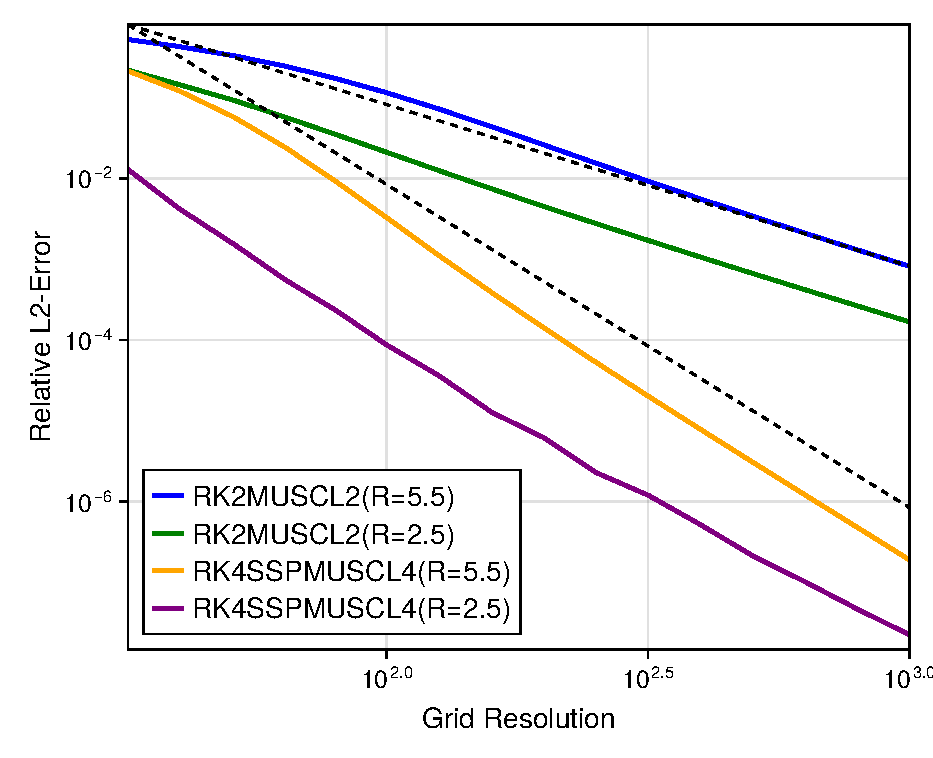
\includegraphics[width=\textwidth]{figures/advection_conv_radius.pdf}
\caption{linear advection, $t=1$}
\end{subfigure}\hfill
\begin{subfigure}{0.48\textwidth}\centering
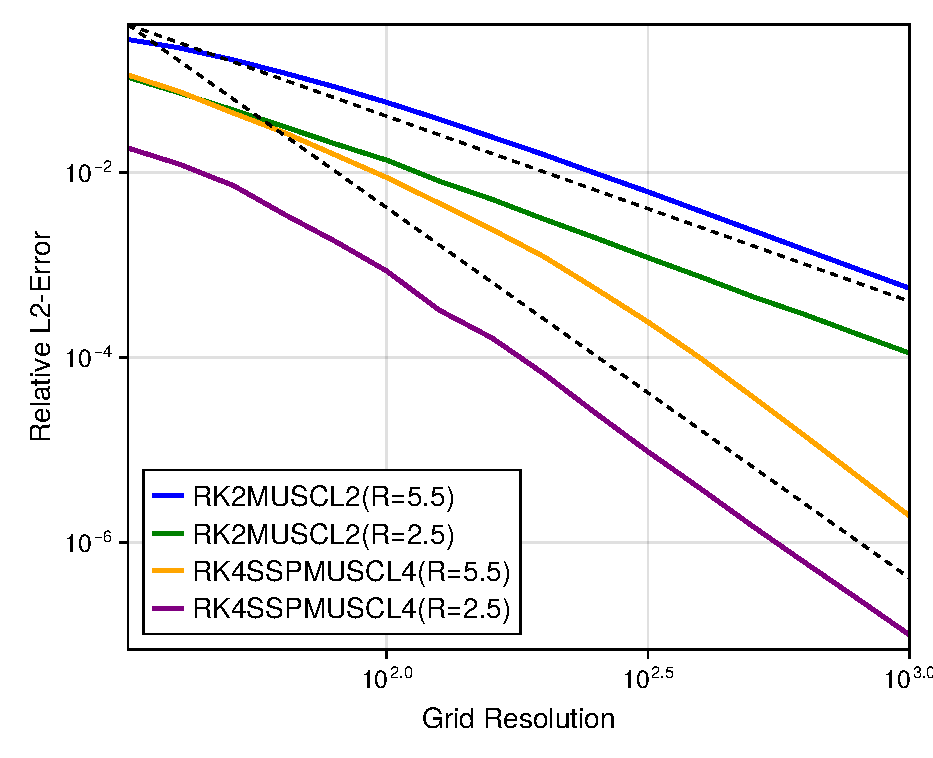
\includegraphics[width=\textwidth]{figures/burgers_conv_radius.pdf}
\caption{Burgers equation, $t=0.5$}
\end{subfigure}
\caption{Relative discrete $L^2$ errors $\big(\sum_i|U_i-u(x_i,t)|^2\big)^{1/2}/\big(\sum_iu(x_i,t)^2\big)^{1/2}$ for the Gaussian pulse in two dimensions on $N\times N$ particles in $[-5,5]^2$ perturbed by $0.2h$ (``grid resolution'' $N$, $h=10/N$), without limiter or MOOD, for RK2MUSCL2 and RK4SSPMUSCL4 with the support radii $R=2.5h$ and $R=5.5h$; dashed lines: slopes $-2$ and $-4$.}\label{fig:convergence}
\end{figure}

The smaller radius $\kappa=2.5$ of the shock computations keeps the design orders on lattices (in two dimensions $2.02$, $3.00$, $4.01$ for advection and $2.06$, $2.98$, $4.12$ for Burgers) with errors at the finest resolution that are $5$ to $30$ times smaller than with $\kappa=5.5$, since the fits weight the near neighbours more strongly; the exception is $K=3$ in one dimension, which falls back to the derivative degree two (\cref{sec:parity}) and is of second order. \Cref{fig:convergence} shows that on the perturbed clouds the radius acts mainly on the error constant. For $K=2$ the curves of both radii are parallel, and at $N=1000$ the relative $L^2$ errors with $\kappa=2.5$ are $4.9$ (advection) and $5.0$ (Burgers) times smaller than with $\kappa=5.5$. For $K=4$ the factors are $8.5$ and $19$. $K=2$ and $K=3$ keep their orders on the perturbed clouds ($1.97$--$2.00$ and $2.91$ in two dimensions, \cref{tab:convergence}), whereas $K=4$ with $\kappa=2.5$ drops to $2.98$ in one dimension, $3.24$ for two-dimensional advection and $3.78$ for Burgers, visible in \cref{fig:convergence} as the less regular slope of the curve RK4SSPMUSCL4($R=2.5$): with $0.2h$ perturbations some stencils of radius $2.5h$ are too close to the minimal size for the degree-three fits. In two dimensions the errors of $K=4$ with $\kappa=2.5$ are nevertheless smaller than with $\kappa=5.5$ over the whole range tested ($1.1\cdot10^{-7}$ instead of $1.4\cdot10^{-6}$ in $L^1$ for Burgers at $N=1000$); in one dimension they are about $20\%$ larger at $N=3163$. For the full order of $K=4$ on perturbed clouds, $\kappa$ between $3.5$ and $5.5$ is needed.

\subsection{Isentropic vortex}\label{sec:vortex}

The isentropic vortex \cite{Shu1998} tests the Euler equations and, in particular, the behaviour of MOOD on a smooth solution with a smooth extremum. A vortex with the strength $\beta=5$ is centred at $(5,5)$ in the periodic domain $[0,10]^2$ on top of the uniform flow $(\rho,u,v,p)=(1,1,1,1)$: with $(\bar x,\bar y)$ the offset from the vortex centre and $r$ its length, the velocity is perturbed by $\frac{\beta}{2\pi}\mathrm{e}^{(1-r^2)/2}(-\bar y,\bar x)$ and the temperature $p/\rho$ by $-\frac{(\gamma-1)\beta^2}{8\gamma\pi^2}\mathrm{e}^{1-r^2}$, with constant entropy $p/\rho^\gamma$. The minimum density in the core is $0.4938$. After one period, $t=10$, the exact solution equals the initial condition. We use $N\times N$ particles, $N=50,71,100,\dots,400$ (factor $\sqrt2$ per step), perturbed by $0.2h$, with $\kappa=2.5$, $\CFL=0.8$ and single precision, and measure the discrete $L^2$ error $\big(h^2\sum_i|\rho_i-\rho_0(x_i)|^2\big)^{1/2}$ of the density, evaluated in double precision. \Cref{tab:vortex} lists the errors, and \cref{tab:vortex_min} the minimum densities, which show directly whether MOOD clips the core.

\begin{table}[!htbp]
\centering
\caption{Isentropic vortex at $t=10$: discrete $L^2$ error of the density and observed order between consecutive resolutions, single precision, perturbation $0.2h$, $\kappa=2.5$.}\label{tab:vortex}
\small
\begin{tabular}{rcccccc}
\toprule
& \multicolumn{2}{c}{RK2MUSCL2(EPD2,MLS2)} & \multicolumn{2}{c}{RK3MUSCL3(EPD2,MLS2)} & \multicolumn{2}{c}{RK3MUSCL3(none,MLS3)}\\
\cmidrule(lr){2-3}\cmidrule(lr){4-5}\cmidrule(lr){6-7}
$N$ & error & order & error & order & error & order\\
\midrule
50 & 5.99e-1 & & 5.79e-1 & & 1.82e-1 & \\
71 & 5.58e-1 & 0.20 & 5.32e-1 & 0.24 & 7.93e-2 & 2.36\\
100 & 4.85e-1 & 0.41 & 4.14e-1 & 0.73 & 3.56e-2 & 2.34\\
141 & 3.71e-1 & 0.79 & 1.90e-1 & 2.27 & 1.52e-2 & 2.48\\
200 & 2.50e-1 & 1.13 & 1.30e-2 & 7.68 & 5.83e-3 & 2.74\\
283 & 1.51e-1 & 1.44 & 5.73e-3 & 2.36 & 2.20e-3 & 2.80\\
400 & 7.21e-2 & 2.14 & 2.60e-3 & 2.28 & 1.16e-3 & 1.85\\
\bottomrule
\end{tabular}
\end{table}

\begin{table}[!htbp]
\centering
\caption{Isentropic vortex at $t=10$: minimum particle density (exact: $0.4938$) and number of time steps at $N=400$, single precision on GPUs.}\label{tab:vortex_min}
\small
\begin{tabular}{lccccc}
\toprule
& $N=100$ & $N=141$ & $N=200$ & $N=400$ & steps ($N=400$)\\
\midrule
RK2MUSCL2(EPD2,MLS2) & 0.8876 & 0.8026 & 0.6989 & 0.5639 & 4014\\
RK3MUSCL3(EPD2,MLS2) & 0.8163 & 0.5121 & 0.4903 & 0.4934 & 4036\\
RK3MUSCL3(none,MLS3) & 0.4881 & 0.4887 & 0.4919 & 0.4936 & 11798\\
RK4SSPMUSCL4(EPD2,MLS2) & 0.8237 & 0.6632 & 0.4936 & 0.4937 & 4037\\
RK4SSPMUSCL4(EPD2,MLS4) & 0.4941 & 0.4944 & 0.4938 & 0.4938 & 11800\\
RK4SSPMUSCL4(none,MLS4) & 0.4941 & 0.4944 & 0.4938 & 0.4938 & 11800\\
\bottomrule
\end{tabular}
\end{table}

Without MOOD, RK3MUSCL3 converges with orders between $2.3$ and $2.8$, and the core is resolved already at $N=100$. In the last refinement step the order drops to $1.85$ at an error of $1.2\cdot10^{-3}$, possibly the onset of a round-off floor of the high-order fits in single precision; we have not checked this in double precision. With MOOD (EPD2) and $k_{\mathrm{div}}=2$, the third-order scheme clips the core on the coarse clouds, with minimum densities of $0.82$ at $N=100$ and $0.51$ at $N=141$ and errors of the size of the vortex itself. From $N=200$ on, i.e.\ from about twenty particles per core radius, the core is intact: the minimum density agrees with that of the unlimited scheme to within $0.002$, and to three digits from $N=283$ on, and the error decreases with orders $2.4$ and $2.3$, at about twice the error of the unlimited scheme. This order is that of the frozen derivative degree one, which makes the scheme formally of second order (\cref{sec:consistency}), not a loss caused by MOOD. RK4SSPMUSCL4(EPD2,MLS2) behaves in the same way, with the same threshold $N=200$. With $k_{\mathrm{div}}=4$, MOOD does not act at all from $N=100$ on in the GPU runs: RK4SSPMUSCL4(EPD2,MLS4) gives the minimum densities and the number of time steps of the unlimited scheme to four digits. In the CPU runs the mass changes differ slightly from those of the unlimited scheme (for instance $-2.80\cdot10^{-5}$ and $-3.01\cdot10^{-5}$ at $N=200$), so there either MOOD acts on a few particles or the runs are not bitwise reproducible; we have not separated the two. Only on the coarsest clouds, $N\le71$, do all MOOD runs clip the core. For $K=2$ no curvature test is available (\cref{sec:criteria}), so the smooth extremum is clipped at every resolution: the minimum density is still $0.56$ at $N=400$, and the order of the error only approaches two in the last step. The mass changes by at most $2.4\cdot10^{-4}$ in all runs, and by at most $5.3\cdot10^{-5}$ for $N\ge200$.

Two features of the detection (\cref{sec:criteria}) keep the core. First, the plain DMP fires in the far field of the vortex: there the density varies across a stencil by only $10^{-6}$ to $10^{-3}$, but it is updated with the divergence of the momentum, whose truncation error is of the same size, and the relaxation $\delta=\delta_0h^2$ shrinks with the resolution, so the guard $\delta^3$ for flat regions does not apply. The plateau test accepts these particles. Second, the u2 criterion tests only the components that violate the DMP, measures the curvatures in the units of the state, and compares their magnitudes only among the nearest neighbours; over the whole stencil of radius $2.5h$ the curvature of the smooth tail varies strongly, and a magnitude test over the whole stencil would reject the smooth extremum. With the plateau threshold $\pi_0=10^{-3}$ the core is kept from about twenty particles per core radius on with $k_{\mathrm{div}}=2$, and from about ten with $k_{\mathrm{div}}=4$, whose smaller truncation error triggers the DMP less often; on coarser clouds a larger threshold is needed (for instance $\pi_0=10^{-2}$ at $N=100$ with $k_{\mathrm{div}}=2$).

\subsection{Mass conservation}\label{sec:mass}

\Cref{sec:conservation} identifies the conservation error of the scheme with the lack of antisymmetry of the volume-weighted derivative weights. We now measure it. Let $m(t)=\bar h^D\sum_{i\in I}U_i$ be the discrete mass with the equal volumes $\bar h^D=|\Omega|/|I|$ of the interior particles,  and let $\Phi(t)$ be the exact time-integrated boundary flux. With equal volumes, the pair defects of \eqref{eq:balance} measure the antisymmetry of the weights $c_{ij}$ themselves; on the perturbed lattice of \cref{tab:stencils} they are $5.7\%$, $16.7\%$ and $72.9\%$ for degree one, degree three and mixed degrees, almost the same as with Shepard volumes. We report the \emph{conservation defect}
\begin{equation}\label{eq:defect}
\delta_m = \frac{m(t_{\mathrm{end}})-m(0)-\Phi(t_{\mathrm{end}})}{m(t_{\mathrm{end}})},
\end{equation}
which vanishes up to round-off for a conservative scheme with exact boundary fluxes. Unlike the relative error with respect to the mass of the exact solution sampled on the particles, $\delta_m$ contains no sampling error of a discontinuous reference. Three scalar problems are used, all with $\CFL=0.2$:
\begin{itemize}
\item a one-dimensional Burgers shock, $u=1$ for $x<-2$ and $u=0$ for $x>-2$ on $[-5,5]$ with transmissive boundaries, up to $t=10$, when the shock, moving with speed $\tfrac12$, has reached $x=3$; here $\Phi=\tfrac12t$;
\item one-dimensional linear advection of the Gaussian of \cref{sec:smooth} with periodic boundaries over one period, $t=10$ ($\Phi=0$);
\item the two-dimensional Burgers problem of \cref{sec:smooth} before shock formation, $t=0.5$ ($\Phi=0$).
\end{itemize}
The one-dimensional sweeps use $N=32,\dots,3163$ and the two-dimensional ones $N=32,\dots,200$ per direction. The clouds are lattices perturbed by $\theta h$ per coordinate with $\theta\in\{0,\dots,0.5\}$, mostly $\theta=0.4$, and $R=\kappa h$ with mostly $\kappa=5.5$ and $\alpha=1$. The schemes use the steppers of \cref{sec:smooth} and the aligned flux; for comparison, all MOOD variants were also run with the geometric orientation (RU). The complete data, including the time histories, are provided as supplementary material. The conservation of the Sod problem is reported in \cref{sec:sod}.

\begin{figure}[!htbp]
\centering
\begin{subfigure}{0.48\textwidth}\centering
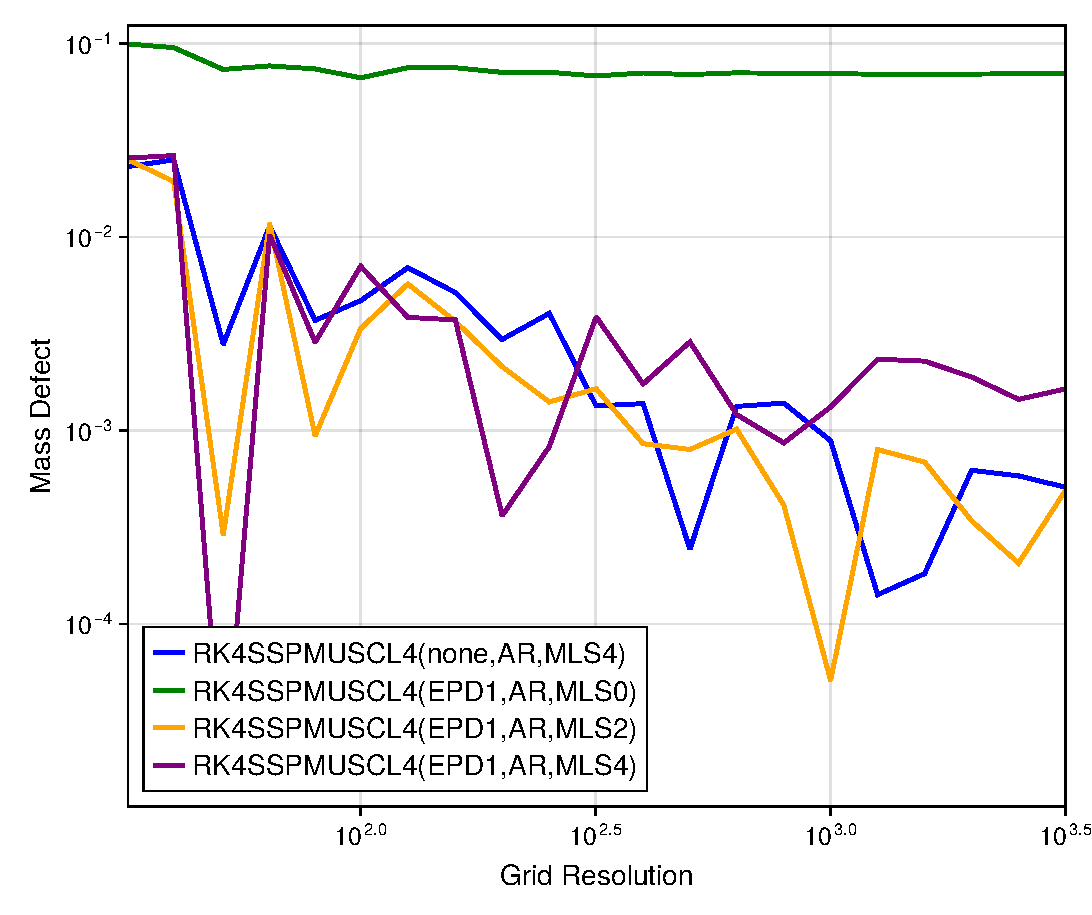
\includegraphics[width=\textwidth]{figures/shock_mass_defect_epd1.pdf}
\caption{MOOD with EPD1}
\end{subfigure}\hfill
\begin{subfigure}{0.48\textwidth}\centering
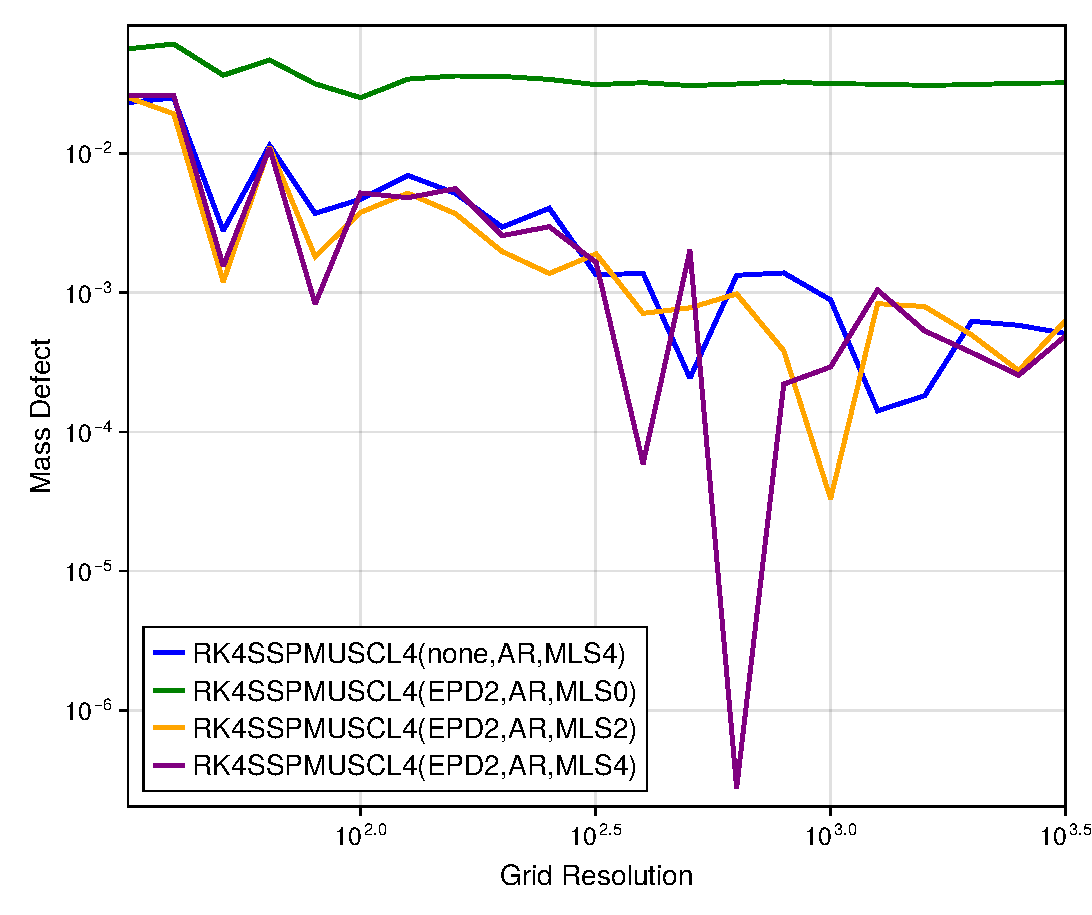
\includegraphics[width=\textwidth]{figures/shock_mass_defect_epd2.pdf}
\caption{MOOD with EPD2}
\end{subfigure}
\caption{Conservation defect $|\delta_m|$ of \eqref{eq:defect} for the one-dimensional Burgers shock, perturbation $0.4h$, $\kappa=5.5$, aligned flux, for RK4SSPMUSCL4 without MOOD (MLS4) and with MOOD in the coupled mode (MLS0) and in the frozen mode with $k_{\mathrm{div}}=2$ (MLS2) and $k_{\mathrm{div}}=4$ (MLS4).}\label{fig:mass}
\end{figure}

\begin{table}[!htbp]
\centering
\caption{Conservation defect \eqref{eq:defect} for the one-dimensional Burgers shock at $N=3163$, perturbation $0.4h$, $\kappa=5.5$, for MUSCL$K$ with the given stabilization and derivative mode (frozen $K$: $k_{\mathrm{div}}=K$; frozen 2: $k_{\mathrm{div}}=2$, derivative degree one), with the aligned flux except for the rows RU, which use the geometric flux. In parentheses: the rate $r$ of a least-squares fit $|\delta_m|\propto N^{-r}$ over $N\ge100$; rates near zero mean that the defect does not decrease with $N$.}\label{tab:mass_shock}
\footnotesize
\setlength{\tabcolsep}{4pt}
\begin{tabular}{llcccc}
\toprule
stabilization & derivative & $K=2$ & $K=3$ & $K=4$ & $K=5$\\
\midrule
none & frozen $K$ & $+$1.1e-4 (1.0) & $+$2.3e-4 (1.0) & $+$5.1e-4 (0.9) & $-$2.3e-3 (0.0)\\
VK limiter & frozen $K$ & $-$4.3e-4 (0.9) & $+$5.1e-4 (0.9) & $-$7.3e-4 (0.8) & $-$3.6e-3 (0.1)\\
minmod limiter & frozen $K$ & $-$3.6e-4 (0.9) & $+$2.0e-3 (0.5) & $+$1.5e-3 (0.7) & $-$3.8e-3 (0.0)\\
\midrule
MOOD, EPD1 & frozen 2 & $-$4.1e-4 (0.9) & $-$4.7e-4 (0.8) & $-$4.9e-4 (0.8) & $-$5.4e-4 (0.8)\\
MOOD, EPD2 & frozen 2 & $-$6.0e-4 (0.7) & $-$7.0e-4 (0.7) & $-$6.3e-4 (0.8) & $-$6.1e-4 (0.7)\\
MOOD, EPD1 & frozen $K$ & $-$4.1e-4 (0.9) & $+$3.1e-4 (0.9) & $-$1.6e-3 (0.2) & $-$7.2e-3 (0.1)\\
MOOD, EPD2 & frozen $K$ & $-$6.0e-4 (0.7) & $+$1.8e-3 (0.8) & $+$4.9e-4 (0.9) & $-$1.3e-3 (0.4)\\
\midrule
MOOD, EPD1 & coupled & $-$4.1e-4 (0.9) & $+$1.2e-1 (0.0) & $+$7.0e-2 (0.0) & $+$1.4e-1 (0.0)\\
MOOD, EPD2 & coupled & $-$6.0e-4 (0.7) & $+$6.3e-2 (0.0) & $+$3.2e-2 (0.0) & $+$7.1e-2 (0.0)\\
MOOD, EPD1 & coupled, RU & $-$4.1e-4 (0.9) & $-$2.8e-2 ($-$0.1) & $+$2.7e-2 (0.0) & $-$2.8e-3 (0.1)\\
MOOD, EPD2 & coupled, RU & $-$5.7e-4 (0.7) & $+$3.4e-2 (0.0) & $+$2.7e-2 (0.0) & $-$5.0e-3 ($-$0.1)\\
\bottomrule
\end{tabular}
\end{table}

\paragraph{The floor of the shock test.} On the unperturbed lattice all frozen and unlimited schemes of this test give the same kind of defect, which is either at most about $2\cdot10^{-5}$ in magnitude, mostly zero to round-off, or exactly $-h\,u_L/(2m(t_{\mathrm{end}}))$, i.e.\ half a particle of the inflow state (for instance $-2.0\cdot10^{-4}$ at $N=3163$), depending on $N$. The interior scheme is exactly conservative on the lattice (\cref{sec:conservation}), so this value reflects how the inflow boundary and the initial discontinuity sit on the lattice rather than the scheme. It decreases like $h$, and defects below a few $10^{-4}$ at $N=3163$ are not resolved by this test.

\paragraph{The frozen mode with degree one.} With the frozen derivative degree $k_{\mathrm{div}}=2$, i.e.\ derivative weights of degree one for every $K$, the conservation defect of MOOD is at the level of the floor for all orders $K=2,\dots,5$ and both interface rules, between $-4.1\cdot10^{-4}$ and $-7.0\cdot10^{-4}$ at $N=3163$, and it decreases under refinement, at fitted rates between $0.7$ and $0.9$ (\cref{fig:mass,tab:mass_shock}). The aligned and the geometric orientation give the same defects to within $7\%$, since for these weights they differ only on the few weights that violate the sign condition (\cref{sec:positivity}).

\paragraph{The coupled mode.} The coupled mode produces mixed-degree pairs at the boundaries of the lowered regions. With the geometric flux it changes the mass for $K=3$ and $K=4$ by $2.7$--$3.4\%$, with either sign, and this defect does not decrease under refinement, in agreement with the defect of $73\%$ of mixed-degree pairs, which is as large on lattices as on perturbed clouds (\cref{tab:stencils}). With the aligned flux, whose orientation is taken from the weights of the degree in use (\cref{sec:fluxes}), the defects are even larger: $3.2$--$14\%$, flat in $N$ (\cref{fig:mass}). The aligned orientation makes the fallback positive, but it does not remove the mixed-degree pairs, which dominate the conservation error. The coupled mode should not be used for $K\ge3$.

\paragraph{The frozen mode with higher degrees.} With $k_{\mathrm{div}}=K$, the aligned flux makes the fallback positive, and there are no mixed-degree pairs. For $K=3$ with EPD1 and $K=4$ with EPD2 the defects at $N=3163$ are $3.1\cdot10^{-4}$ and $4.9\cdot10^{-4}$ and decrease at rates of about $0.9$, like those of the unstabilized schemes; for $K=3$ with EPD2 the defect is $1.8\cdot10^{-3}$ at a rate of $0.8$. With EPD1, defects of $1.6\cdot10^{-3}$ for $K=4$ and $7.2\cdot10^{-3}$ for $K=5$ decrease only slowly or not at all in the range tested; in \cref{fig:mass}a the defect of RK4SSPMUSCL4(EPD1,MLS4) stays between $8.6\cdot10^{-4}$ and $2.3\cdot10^{-3}$ for $N\ge631$, while the variants with $k_{\mathrm{div}}=2$ and without MOOD continue to decrease. For $K=5$ the degree-five derivative fit has six unknowns in one dimension and therefore requires $1.5\cdot6=9$ neighbours (\cref{sec:parity}); at $\theta=0.4$ and $\kappa=5.5$ some stencils have fewer, fall back to degree four and create mixed-degree pairs, which also explains the flat defects of the unstabilized scheme and of the limiters at $K=5$ ($2$--$4\cdot10^{-3}$). For $K=4$ the cause is open (\cref{sec:open}).

\paragraph{Irregularity, support and weight.} On the shock problem the perturbation alone costs a few $10^{-4}$: for $\theta=0.1,\dots,0.5$ the defects of the unstabilized schemes with $K=2$ and $K=4$ lie between $1.0\cdot10^{-4}$ and $8.0\cdot10^{-4}$. MUSCL4(EPD1) with $k_{\mathrm{div}}=4$ is more sensitive to the perturbation ($-2.0\cdot10^{-3}$ at $\theta=0.5$), to the radius ($+2.5\cdot10^{-3}$ for $\kappa=3.5$, $-6.5\cdot10^{-4}$ for $\kappa=9.5$) and to the weight parameter $\alpha\in[0.5,4]$ (changes of up to $1.1\cdot10^{-3}$). For smooth periodic solutions in one dimension the perturbation-induced defect is negligible, at most $7.4\cdot10^{-8}$ at $N=3163$. In two dimensions (\cref{tab:mass_2d}) the lattice is exactly conservative, while the perturbed clouds have defects of about $10^{-4}$ at $N=200$ on smooth data, roughly proportional to $\theta$, nearly independent of $K$ and of the stabilization, and decreasing with fitted rates between $1.0$ and $2.0$. This is the static asymmetry $V_ic_{ij}\ne-V_jc_{ji}$ of the stencils on irregular clouds (\cref{tab:stencils}), which acts like a truncation error.

\begin{table}[!htbp]
\centering
\caption{Conservation defect \eqref{eq:defect} for the two-dimensional periodic Burgers problem at $N=200$ ($4\cdot10^4$ particles), frozen derivative degree $k_{\mathrm{div}}=K$, without stabilization, with MOOD (EPD1) and with the VK limiter, for perturbation amplitudes $\theta h$ and support radii $\kappa h$ (in parentheses: fitted rate of $|\delta_m|$ over $N\ge100$). On the unperturbed lattice $|\delta_m|\le3\cdot10^{-16}$ for all variants.}\label{tab:mass_2d}
\footnotesize
\setlength{\tabcolsep}{3.5pt}
\begin{tabular}{cccccccc}
\toprule
& & \multicolumn{3}{c}{$K=2$} & \multicolumn{3}{c}{$K=4$}\\
\cmidrule(lr){3-5}\cmidrule(lr){6-8}
$\theta$ & $\kappa$ & none & EPD1 & VK & none & EPD1 & VK\\
\midrule
0.2 & 3.5 & $+$8.3e-5 (1.9) & $+$7.4e-5 (2.0) & $+$7.9e-5 (2.0) & $+$1.1e-4 (1.2) & $+$1.1e-4 (1.2) & $+$1.1e-4 (1.3)\\
0.2 & 5.5 & $+$1.4e-4 (1.2) & $+$1.3e-4 (1.3) & $+$1.3e-4 (1.0) & $+$1.1e-4 (1.4) & $+$1.1e-4 (1.4) & $+$1.1e-4 (1.1)\\
0.4 & 3.5 & $+$2.2e-4 (1.5) & $+$2.1e-4 (1.5) & $+$2.2e-4 (1.6) & $+$2.2e-4 (1.2) & $+$2.2e-4 (1.2) & $+$2.2e-4 (1.6)\\
0.4 & 5.5 & $+$2.6e-4 (1.3) & $+$2.5e-4 (1.3) & $+$2.6e-4 (1.1) & $+$2.3e-4 (1.3) & $+$2.3e-4 (1.3) & $+$2.4e-4 (1.1)\\
\bottomrule
\end{tabular}
\end{table}

\paragraph{Why mixed degrees do not converge and equal degrees do.} The mechanism is visible in \eqref{eq:balance}. For a smooth solution the interface fluxes are smooth functions of the midpoints, and the interior sum is a consistent quadrature of a vanishing quantity whose error decreases with $h$. At a discontinuity the fluxes of the pairs that straddle it jump by $O([F])$, and in one dimension $O(\kappa^2)$ such pairs with pair defects $|d_{ij}|=O(\varepsilon)$ change the mass at a rate $O(\varepsilon[F])$ independent of $h$. Whether this rate accumulates depends on its sign. At the boundary of a lowered region, the pairs of a high-degree and a low-degree particle have the same geometric arrangement wherever the shock is, so their defects have a systematic sign, and the mass error grows in time and does not decrease under refinement. With equal degrees on a randomly perturbed cloud, the defects of the pairs at the shock change sign at random as the shock passes from particle to particle, and their contributions largely cancel; the integrated error then decreases under refinement, which is what we observe. This heuristic is consistent with the flat defects of the coupled mode and with the decreasing defects of the frozen mode, but it does not predict a rate.

\subsection{The Sod shock tube}\label{sec:sod}

As a one-dimensional test for systems we use the shock tube of Sod \cite{Sod1978}: $(\rho,u,p)=(1,0,1)$ for $x<0$ and $(0.125,0,0.1)$ for $x>0$ on $[-0.5,0.5]$, $\gamma=1.4$, up to $t=0.2$, with a Dirichlet condition on the left and a transmissive condition on the right. The clouds are lattices perturbed by $0.2h$ with $N=100,\dots,1000$ particles (eleven resolutions), $\kappa=5.5$, $\alpha=1$ and $\CFL=0.2$. We compare RK2MUSCL1, RK2MUSCL2 with EPD1, EPD2 and the VK limiter, and RK3MUSCL3 and RK4SSPMUSCL4 with EPD1 and EPD2 in the frozen mode with $k_{\mathrm{div}}=2$ and $k_{\mathrm{div}}=K$, all with the aligned flux except RK2MUSCL1. The errors are measured against the exact Riemann solution. \Cref{fig:sod} shows the profiles at $N=200$ and \cref{tab:sod} the errors.

\begin{figure}[!htbp]
\centering
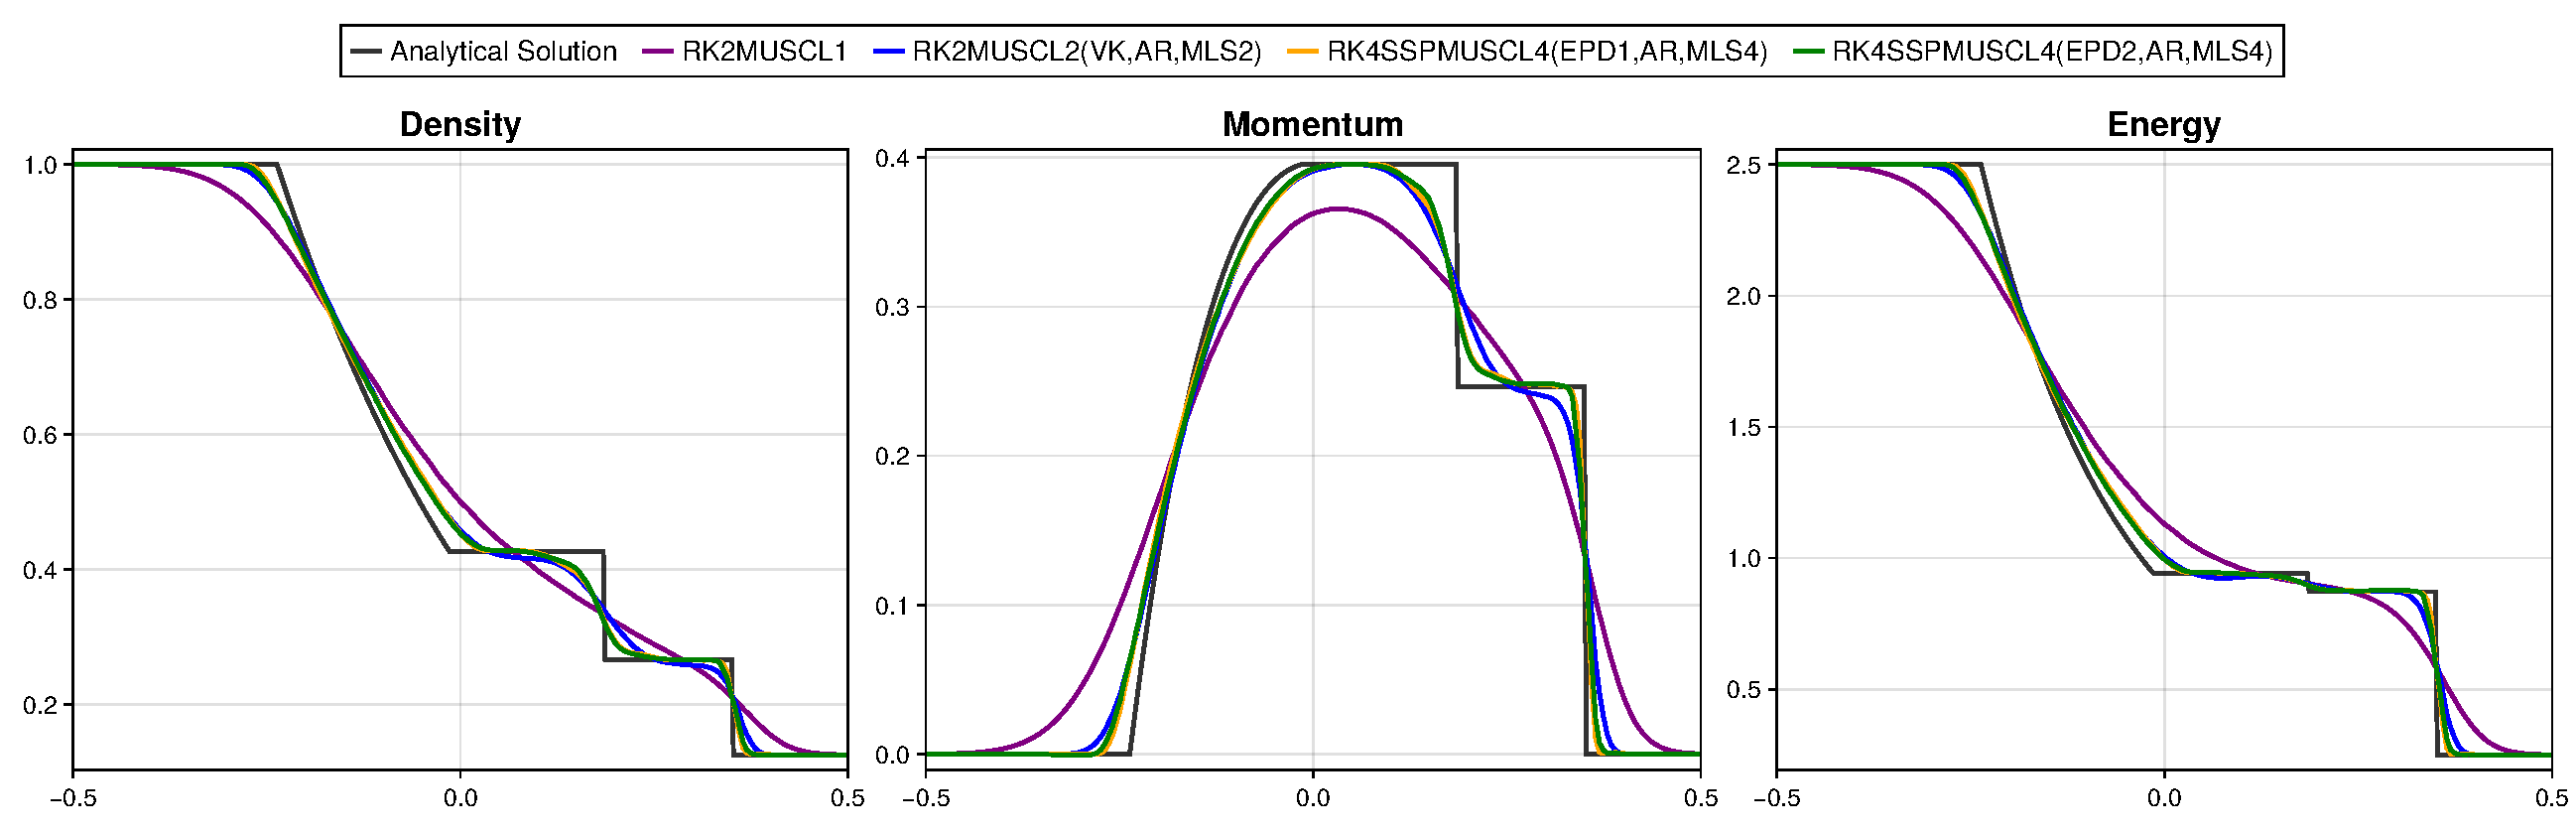
\includegraphics[width=\textwidth]{figures/euler_sod_components.pdf}
\caption{Sod shock tube at $t=0.2$ on $N=200$ particles perturbed by $0.2h$, $\kappa=5.5$: density, momentum and energy of RK2MUSCL1, RK2MUSCL2(VK,MLS2), RK4SSPMUSCL4(EPD1,MLS4) and RK4SSPMUSCL4(EPD2,MLS4), and the exact solution; all schemes except RK2MUSCL1 use the aligned flux.}\label{fig:sod}
\end{figure}

\begin{table}[!htbp]
\centering
\caption{Sod shock tube at $t=0.2$, perturbation $0.2h$, $\kappa=5.5$: discrete $L^1$ and $L^2$ errors of the density against the exact solution, observed orders between $N=502$ and $N=1000$, and the relative mass change $m(t)/m(0)-1$ at $N=1000$.}\label{tab:sod}
\footnotesize
\setlength{\tabcolsep}{4pt}
\begin{tabular}{lccccccc}
\toprule
& \multicolumn{4}{c}{$L^1(\rho)$} & \multicolumn{2}{c}{$L^2(\rho)$} & \\
\cmidrule(lr){2-5}\cmidrule(lr){6-7}
& $N=100$ & $N=317$ & $N=1000$ & order & $N=1000$ & order & mass, $N=1000$\\
\midrule
RK2MUSCL1 & 4.51e-2 & 2.91e-2 & 1.55e-2 & 0.59 & 2.49e-2 & 0.42 & $+$2.5e-5\\
RK2MUSCL2(EPD1,MLS2) & 2.63e-2 & 1.32e-2 & 4.68e-3 & 0.87 & 1.17e-2 & 0.55 & $+$3.3e-5\\
RK2MUSCL2(EPD2,MLS2) & 3.06e-2 & 1.52e-2 & 5.49e-3 & 0.92 & 1.28e-2 & 0.57 & $+$3.2e-5\\
RK2MUSCL2(VK,MLS2) & 2.97e-2 & 1.05e-2 & 3.57e-3 & 0.97 & 1.01e-2 & 0.52 & $+$3.1e-5\\
RK3MUSCL3(EPD1,MLS2) & 2.89e-2 & 1.00e-2 & 3.30e-3 & 1.00 & 1.02e-2 & 0.54 & $+$3.3e-5\\
RK3MUSCL3(EPD2,MLS2) & 2.97e-2 & 1.49e-2 & 5.25e-3 & 0.92 & 1.26e-2 & 0.57 & $+$3.3e-5\\
RK3MUSCL3(EPD1,MLS3) & 2.81e-2 & 9.64e-3 & 3.16e-3 & 1.00 & 9.62e-3 & 0.57 & $+$6.0e-5\\
RK3MUSCL3(EPD2,MLS3) & 2.84e-2 & 9.48e-3 & 3.12e-3 & 1.02 & 9.49e-3 & 0.57 & $+$1.2e-4\\
RK4SSPMUSCL4(EPD1,MLS2) & 2.58e-2 & 8.67e-3 & 2.80e-3 & 1.00 & 9.61e-3 & 0.51 & $+$3.2e-5\\
RK4SSPMUSCL4(EPD2,MLS2) & 2.88e-2 & 1.41e-2 & 4.93e-3 & 0.93 & 1.18e-2 & 0.58 & $+$3.6e-5\\
RK4SSPMUSCL4(EPD1,MLS4) & 2.56e-2 & 8.18e-3 & 2.65e-3 & 1.05 & 8.24e-3 & 0.61 & $+$8.0e-5\\
RK4SSPMUSCL4(EPD2,MLS4) & 2.59e-2 & 8.27e-3 & 2.72e-3 & 1.06 & 8.39e-3 & 0.61 & $+$1.0e-4\\
\bottomrule
\end{tabular}
\end{table}

All 132 runs reach the final time with positive density and pressure; the minimum density is that of the exact right state, $0.125$, in all runs except RK2MUSCL2(EPD1), where it is $0.1249$. For every scheme with $K\ge2$ the $L^1$ error decreases with orders between $0.87$ and $1.06$, the rate expected for a solution with a shock, and the $L^2$ error with orders between $0.51$ and $0.61$; RK2MUSCL1 is not yet in its asymptotic range ($0.59$). The frozen mode with $k_{\mathrm{div}}=K$ gives the smallest errors, $3.1\cdot10^{-3}$ for $K=3$ and $2.7\cdot10^{-3}$ for $K=4$ at $N=1000$, $5.0$ and $5.8$ times less than RK2MUSCL1. With $k_{\mathrm{div}}=2$, EPD2 gains little over the second-order scheme ($5.2\cdot10^{-3}$ and $4.9\cdot10^{-3}$ for $K=3,4$, compared with $5.5\cdot10^{-3}$ for $K=2$), EPD1 more ($3.3\cdot10^{-3}$ and $2.8\cdot10^{-3}$, compared with $4.7\cdot10^{-3}$). At $K=2$ the VK limiter ($3.6\cdot10^{-3}$) is more accurate than both MOOD variants. In \cref{fig:sod} the fourth-order schemes resolve the contact discontinuity and the shock over a few particles, with at most small overshoots, while RK2MUSCL1 smears all three waves; RK2MUSCL2(VK) lies in between, with a visibly wider contact and shock. Since the waves stay inside the domain and $u=0$ in both boundary states, the exact mass is constant. Near both boundaries the state stays constant, so that the zero row sums make the updates there vanish and the boundaries cannot change the mass. The measured mass changes of $2.5\cdot10^{-5}$ to $1.2\cdot10^{-4}$ at $N=1000$ are therefore the static asymmetry of the derivative weights at the moving shock and contact (\cref{sec:mass}); they are largest with $k_{\mathrm{div}}=K$, whose degree-three weights have the larger pair defects (\cref{tab:stencils}).

\subsection{Two-dimensional shock problems}\label{sec:euler2d}

The two-dimensional Riemann problem, the double Mach reflection and the Mach~3 step were computed with the first-order baseline RK2MUSCL1 (plain Rusanov flux) and, with the aligned flux, MUSCL2 with EPD1, EPD2 and the VK limiter, and MUSCL3 and MUSCL4 with EPD1 and EPD2 in the frozen mode with $k_{\mathrm{div}}=2$ and $k_{\mathrm{div}}=K$ and in the coupled mode, and MUSCL2 to MUSCL4 with EPD2 and $k_{\mathrm{div}}=2$ also with the geometric flux; the coupled MUSCL4 runs of the double Mach reflection use $960\times300$ particles. \Cref{tab:euler2d} summarizes positivity and mass. All 57 runs, and the three Riemann runs with transmissive boundaries of \cref{sec:riemann}, reach the final time with positive density and pressure and without invalid values, including the coupled mode. The lowest pressure of all runs, $4.8\cdot10^{-3}$, occurs on the step for $K=3$ with $k_{\mathrm{div}}=K$ and EPD1, positive but close to vacuum, where the shock meets the wall above the step. The frozen mode with $k_{\mathrm{div}}=2$ and EPD2 is the most robust choice, with $\min p\ge0.249$ on the step for every $K$. On the Riemann problem, the minimum pressures of the second- to fourth-order schemes, $0.018$ to $0.029$, undershoot the lowest initial pressure $0.029$ by up to $39\%$. With $k_{\mathrm{div}}=2$ the aligned and the geometric flux agree to within about $4\%$ in all quantities of \cref{tab:euler2d} (the largest difference is in the minimum pressure on the step, $0.27$ and $0.28$ for $K=3$, $0.28$ and $0.29$ for $K=4$), and the high-order schemes take as many time steps as the second-order scheme ($13.5$--$13.7\times10^3$ on the step, compared with $13.5\times10^3$ for RK2MUSCL2 and $13.1\times10^3$ for RK2MUSCL1); with $k_{\mathrm{div}}=K$ and in the coupled mode they take about three times as many, $4.04$--$4.09\times10^4$ (\cref{sec:timestep}).

In the frozen mode the final masses agree with that of RK2MUSCL2(EPD1) to within $0.25\%$ on all three problems. Since the problems have inflow and outflow boundaries, the reference is a computed mass, and the masses are known to three digits, i.e.\ to about $0.1\%$. The coupled mode with EPD1 is not conservative: its final mass differs by $-3.5\%$ on the step, by $+5.4\%$ ($K=3$) and $+4.7\%$ ($K=4$) on the double Mach reflection and by $+1.4\%$ ($K=3$) on the Riemann problem, consistent with \cref{sec:mass}; with EPD2 the differences are smaller, $-2.0$ to $+0.8\%$.

\begin{table}[!htbp]
\centering
\caption{Two-dimensional shock problems: minimum particle pressure and final mass relative to RK2MUSCL2(EPD1,AR,MLS2) (total masses known to about $0.1\%$). Pairs of values: EPD1 / EPD2. All runs except RK2MUSCL1 with the aligned flux. $^*$: $960\times300$ particles; the mass is still compared with the $1440\times450$ run of RK2MUSCL2(EPD1).}\label{tab:euler2d}
\scriptsize
\setlength{\tabcolsep}{2.5pt}
\begin{tabular}{@{}lcccccc@{}}
\toprule
& \multicolumn{2}{c}{Mach 3 step} & \multicolumn{2}{c}{double Mach reflection} & \multicolumn{2}{c}{2-D Riemann problem}\\
\cmidrule(lr){2-3}\cmidrule(lr){4-5}\cmidrule(lr){6-7}
& $\min p$ & mass (\%) & $\min p$ & mass (\%) & $\min p$ & mass (\%)\\
\midrule
RK2MUSCL1 & 1.00 & $+0.1$ & 1.00 & $-0.2$ & 0.029 & $0.0$\\
\begin{tabular}[t]{@{}l@{}}MUSCL2\\ \quad EPD1 / EPD2 / VK\end{tabular} & \begin{tabular}[t]{@{}c@{}}\\ 0.19\,/\,0.25\,/\,0.24\end{tabular} & \begin{tabular}[t]{@{}c@{}}\\ $0.0$\,/\,$-0.2$\,/\,$+0.1$\end{tabular} & \begin{tabular}[t]{@{}c@{}}\\ 1.00\end{tabular} & \begin{tabular}[t]{@{}c@{}}\\ $0.0$\end{tabular} & \begin{tabular}[t]{@{}c@{}}\\ 0.024\,/\,0.029\,/\,0.027\end{tabular} & \begin{tabular}[t]{@{}c@{}}\\ $0.0$\end{tabular}\\
MUSCL3, $k_{\mathrm{div}}=2$ & 0.20 / 0.27 & $+0.1$ / $-0.2$ & 1.00 & $0.0$ & 0.020 / 0.028 & $0.0$\\
MUSCL3, $k_{\mathrm{div}}=3$ & 0.0048 / 0.081 & $-0.1$ / $-0.2$ & 0.96 / 0.99 & $-0.2$ / $0.0$ & 0.018 / 0.026 & $0.0$ / $+0.1$\\
MUSCL3, coupled & 0.014 / 0.067 & $-3.5$ / $-2.0$ & 0.96 / 0.99 & $+5.4$ / $+0.7$ & 0.023 / 0.026 & $+1.4$ / $-0.3$\\
MUSCL4, $k_{\mathrm{div}}=2$ & 0.11 / 0.28 & $+0.1$ / $-0.1$ & 1.00 & $0.0$ & 0.026 / 0.029 & $0.0$\\
MUSCL4, $k_{\mathrm{div}}=4$ & 0.034 / 0.28 & $0.0$ / $+0.1$ & 0.91 / 0.97 & $-0.2$ / $0.0$ & 0.022 / 0.027 & $-0.1$ / $+0.1$\\
MUSCL4, coupled & 0.040 / 0.27 & $-3.5$ / $+0.8$ & 0.88$^*$ / 0.96$^*$ & $+4.7^*$ / $+0.2^*$ & 0.019 / 0.027 & $+0.4$ / $-0.1$\\
\bottomrule
\end{tabular}
\end{table}

\subsection{A two-dimensional Riemann problem}\label{sec:riemann}

Two-dimensional Riemann problems with four constant states in the quadrants of $[0,1]^2$ were classified by Zhang and Zheng \cite{ZhangZheng1990}, Schulz-Rinne \cite{SchulzRinne1993class} and Chang, Chen and Yang \cite{ChangChenYang1995,ChangChenYang2000}, computed systematically by Schulz-Rinne, Collins and Glaz \cite{SchulzRinne1993} and by Lax and Liu \cite{LaxLiu1998}, whose numbering we follow, and have become standard benchmarks for shock-capturing schemes \cite{KurganovTadmor2002}. We use Configuration~3 of \cite{LaxLiu1998,KurganovTadmor2002}, in which every pair of adjacent quadrants is connected by a single shock. With the discontinuities at $x=0.5$ and $y=0.5$, the initial states $(\rho,u,v,p)$ are
\[
\begin{array}{ll}
(0.5323,\,1.206,\,0,\,0.3) & (1.5,\,0,\,0,\,1.5)\\
(0.138,\,1.206,\,1.206,\,0.029) & (0.5323,\,0,\,1.206,\,0.3)
\end{array}
\]
in the upper left, upper right, lower left and lower right quadrants, and the solution is computed until $t=0.3$. Away from the centre the solution consists of plane shocks, whose positions follow from the Rankine--Hugoniot conditions: the shocks bounding the upper right state move with speed $-0.663$ and lie at $x=0.301$ and $y=0.301$ at $t=0.3$, and the shocks bounding the low-density lower left state move with speed $-0.422$ and lie at $x=0.373$ and $y=0.373$. The ghost particles carry these exact plane-shock states on all four sides. Near the centre the shocks interact: the two shocks bounding the low-density state are joined by a curved shock between two triple points, and along the diagonal a mushroom-shaped jet with two roll-ups forms. The problem is symmetric with respect to the diagonal $x=y$.

\begin{figure}[!htbp]
\centering
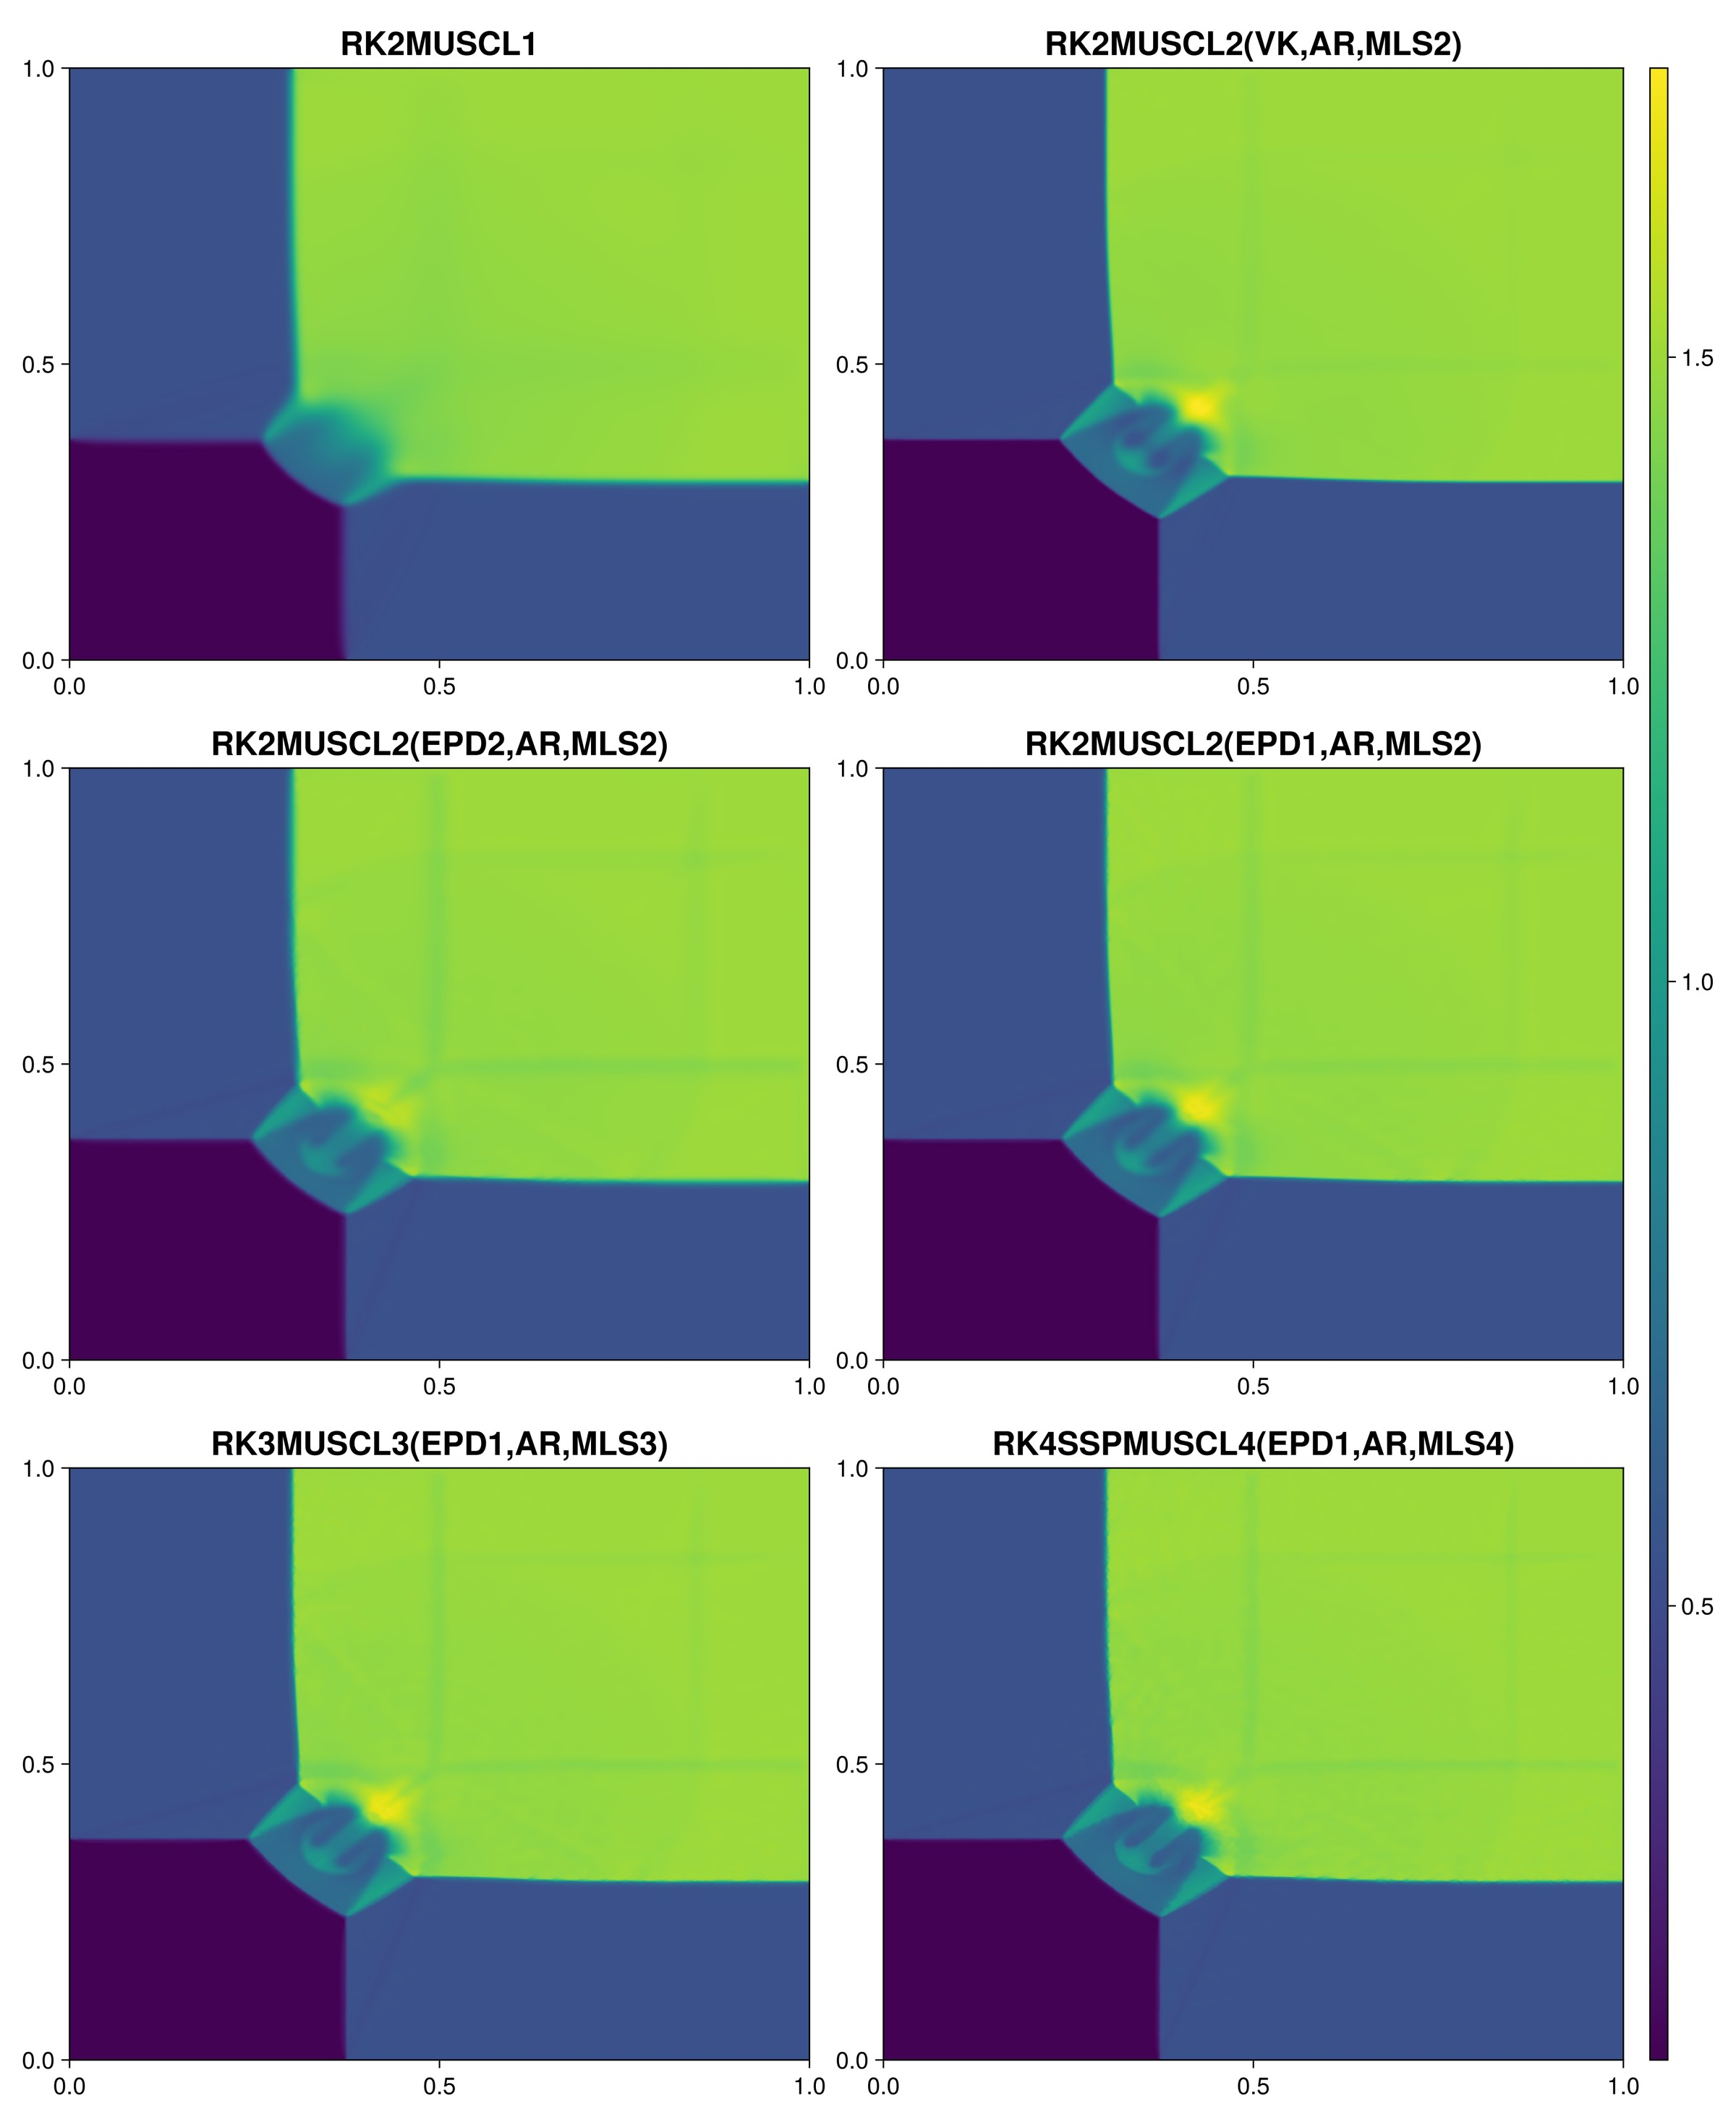
\includegraphics[width=0.74\textwidth]{figures/riemann2d_density_078.jpg}
\caption{Two-dimensional Riemann problem (Configuration~3), density at $t=0.3$ on $800\times800$ particles perturbed by $0.2h$, with a common colour scale, for RK2MUSCL1, RK2MUSCL2 with the VK limiter, EPD2 and EPD1, RK3MUSCL3(EPD1,MLS3) and RK4SSPMUSCL4(EPD1,MLS4); all schemes except RK2MUSCL1 use the aligned flux.}\label{fig:riemann}
\end{figure}

\begin{figure}[!htbp]
\centering
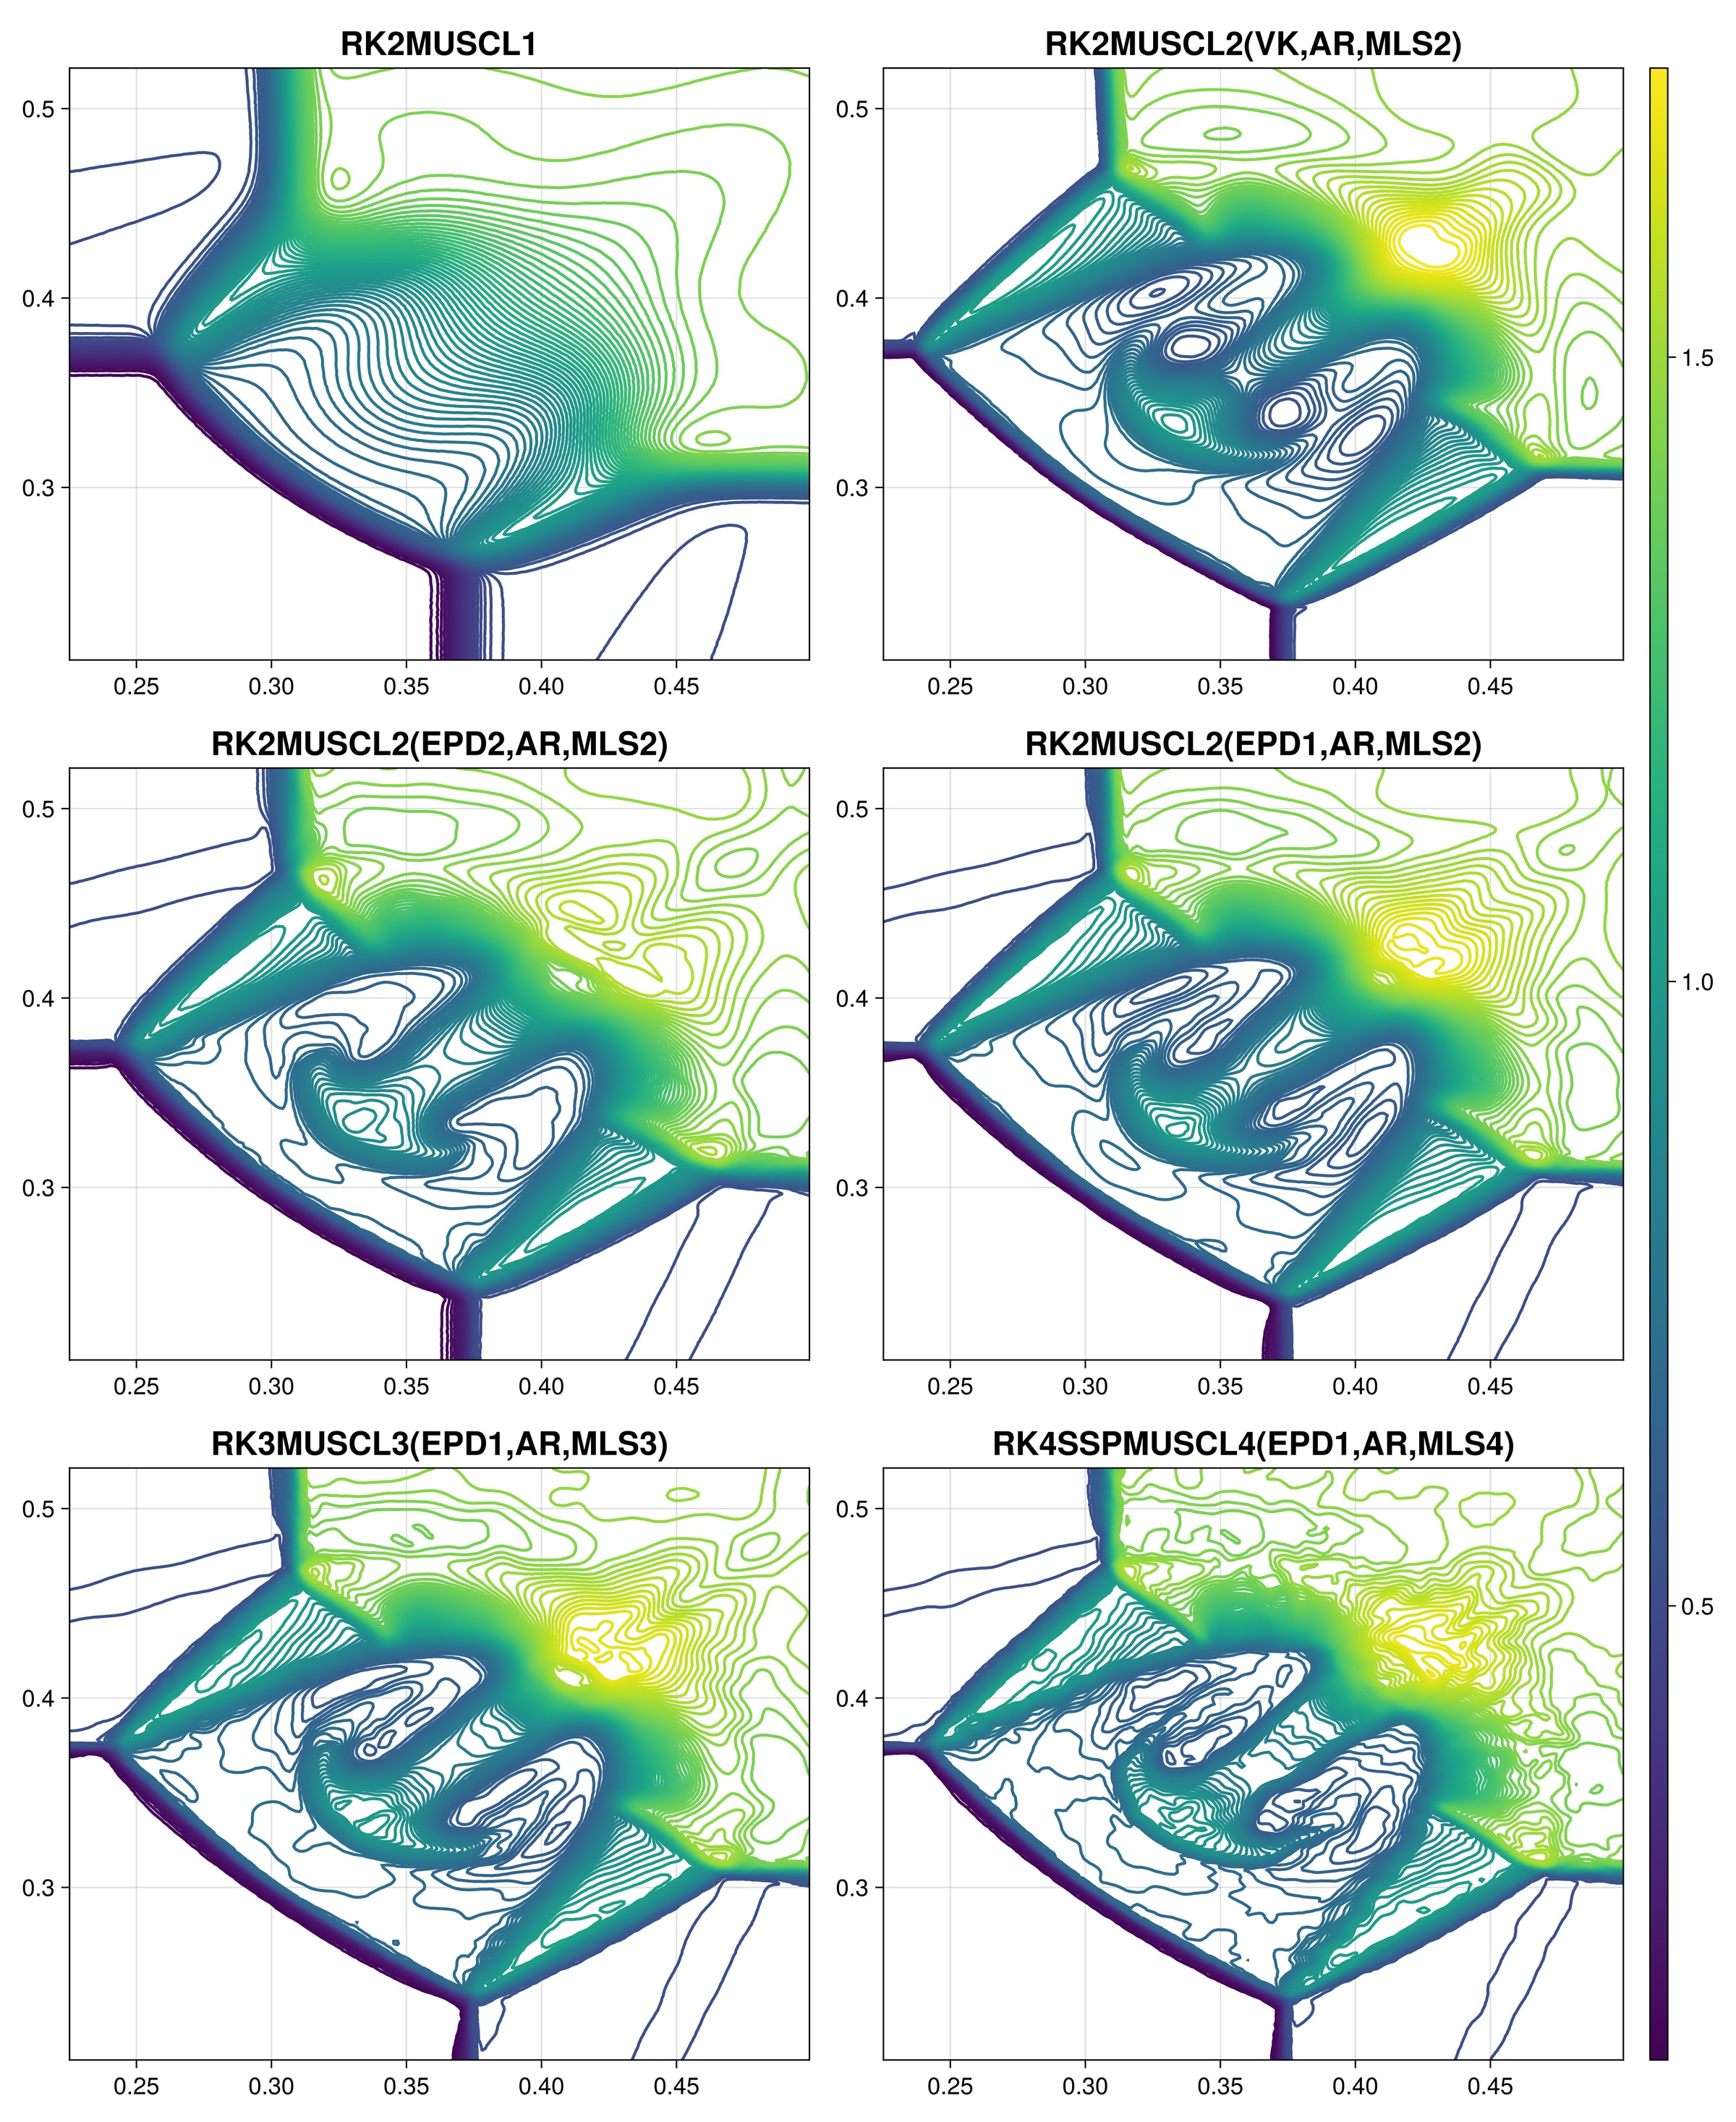
\includegraphics[width=0.74\textwidth]{figures/riemann2d_zoom_078.jpg}
\caption{Two-dimensional Riemann problem: detail $[0.225,0.5]\times[0.21,0.52]$ of \cref{fig:riemann} with $100$ contour levels.}\label{fig:riemannzoom}
\end{figure}

\Cref{fig:riemann,fig:riemannzoom} show the density at $t=0.3$. All runs reproduce the expected wave pattern. With the exact boundary states, the shocks are straight up to the boundaries and lie close to their exact positions, $0.373$ and $0.301$, symmetric with respect to the diagonal. With transmissive instead of exact boundary states, the final mass of the EPD2 runs with $k_{\mathrm{div}}=2$ is $0.6\%$ ($K=2,3$) and $0.9\%$ ($K=4$) lower, a boundary effect that does not concern the interior scheme.

The resolution of the jet along the diagonal differs between the schemes. RK2MUSCL1 smears the cap of the jet into a single blob without roll-ups. The second-order runs resolve the two roll-ups of the mushroom cap; the third- and fourth-order runs resolve them with sharper gradients and a thinner stem. EPD1 and the VK limiter produce a local density maximum of about $1.7$ next to the jet, at about $(0.43,0.43)$, which EPD2 smears. This maximum is part of the solution: the reference computations on $400^2$ and $800^2$ cells give $1.78$ and $1.75$ at the same place. In the contour lines of \cref{fig:riemannzoom} the fourth-order run shows small-scale noise in the upper right state next to the jet. The MOOD runs show faint lines along $x=0.5$ and $y=0.5$ in the upper right state of \cref{fig:riemann}, traces of the initial discontinuities in the fluid at rest, a start-up error common to shock-capturing schemes \cite{LiskaWendroff2003}. In \cref{fig:riemannzoom} faint straight contour lines run from the interaction region towards the lower right; we have not identified their origin.

\subsection{Double Mach reflection}\label{sec:dmr}

The double Mach reflection of Woodward and Colella \cite{Woodward1984} describes a Mach 10 shock that hits a $30^\circ$ wedge, so that the shock makes an angle of $60^\circ$ with the wall. In the frame of the wall, the shock initially lies on the line $x=\tfrac16+y/\sqrt3$ and separates the pre-shock state $(\rho,u,v,p)=(1.4,0,0,1)$ on the right from the post-shock state $(8,\,8.25\cos30^\circ,\,-8.25\sin30^\circ,\,116.5)$ on the left. At the bottom, the post-shock state is prescribed for $x<\tfrac16$ and a slip wall for $x\ge\tfrac16$; at the top, the ghost particles carry the exact states of the moving incident shock, $x_s(y,t)=\tfrac16+(y+20t)/\sqrt3$; the left boundary is an inflow of the post-shock state and the right boundary is transmissive. We use the reduced domain $[0,3.2]\times[0,1]$ instead of the domain $[0,4]\times[0,1]$ of Woodward and Colella; it contains all waves until $t=0.2$.

\begin{figure}[!htbp]
\centering
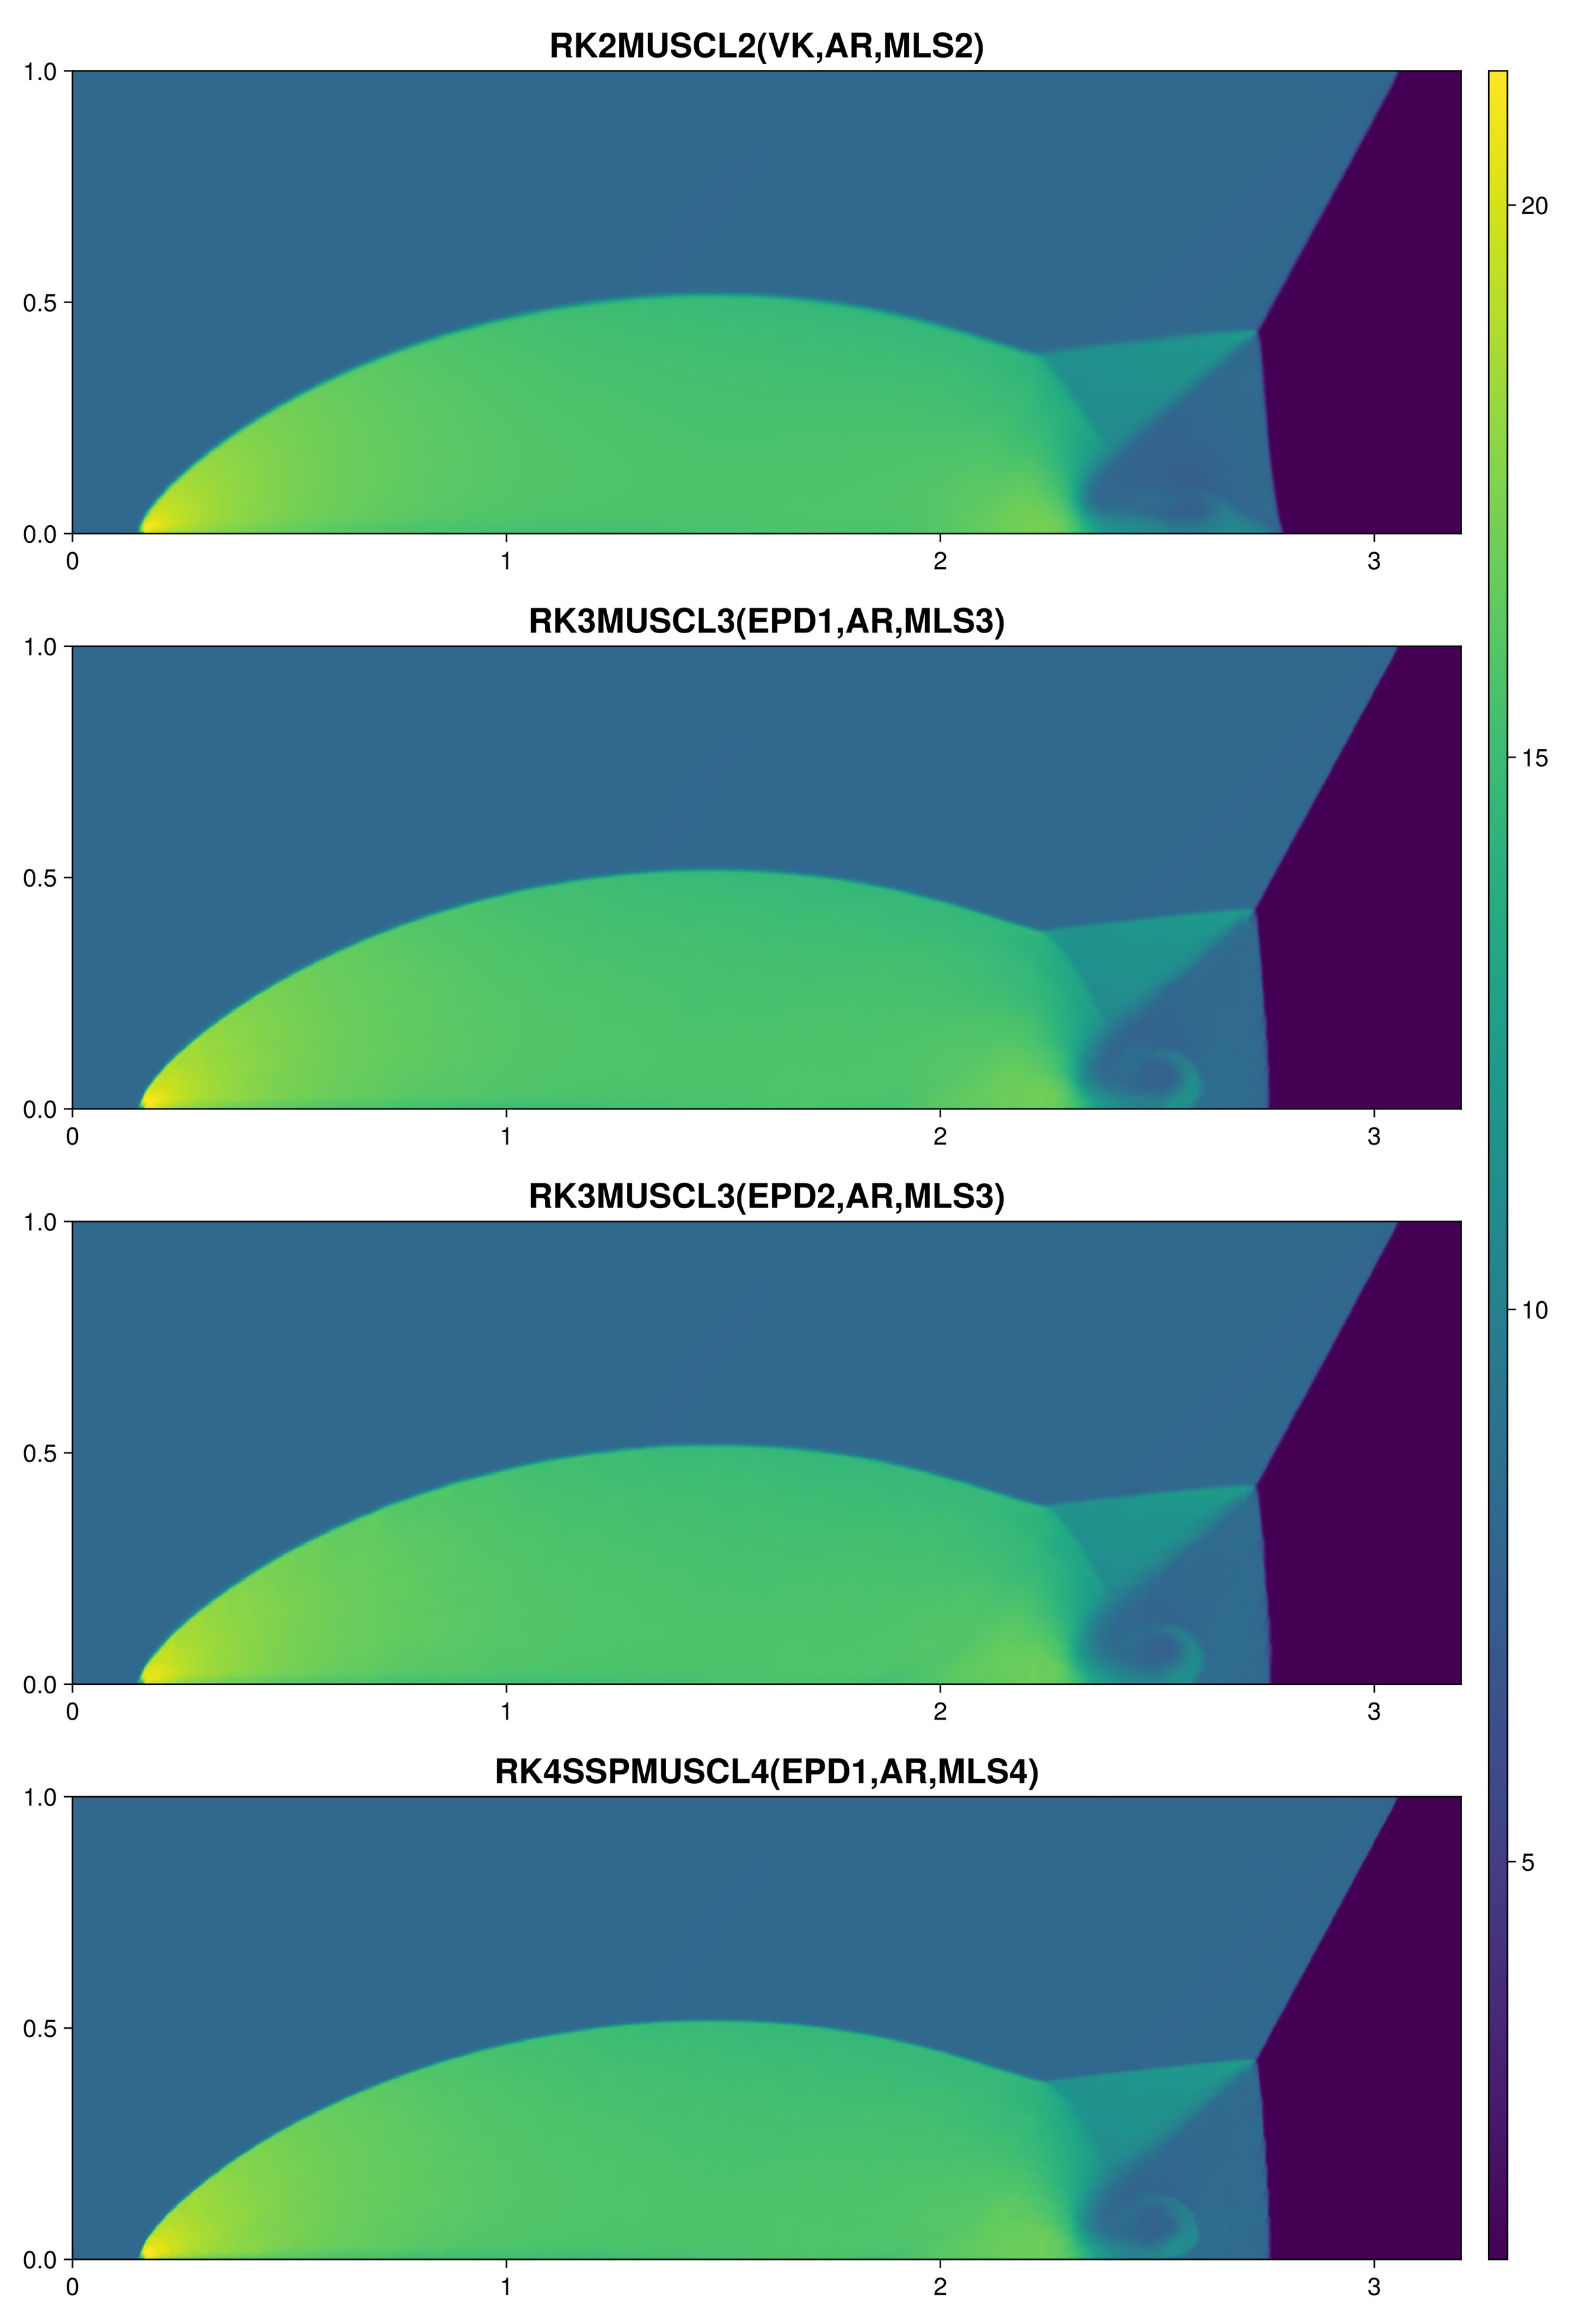
\includegraphics[width=0.68\textwidth]{figures/dmr_density_078.jpg}
\caption{Double Mach reflection, density at $t=0.2$ on $1440\times450$ particles perturbed by $0.2h$ for RK2MUSCL2(VK), RK3MUSCL3(EPD1,MLS3), RK3MUSCL3(EPD2,MLS3) and RK4SSPMUSCL4(EPD1,MLS4), all with the aligned flux, with a common colour scale.}\label{fig:dmr}
\end{figure}

\begin{figure}[!htbp]
\centering
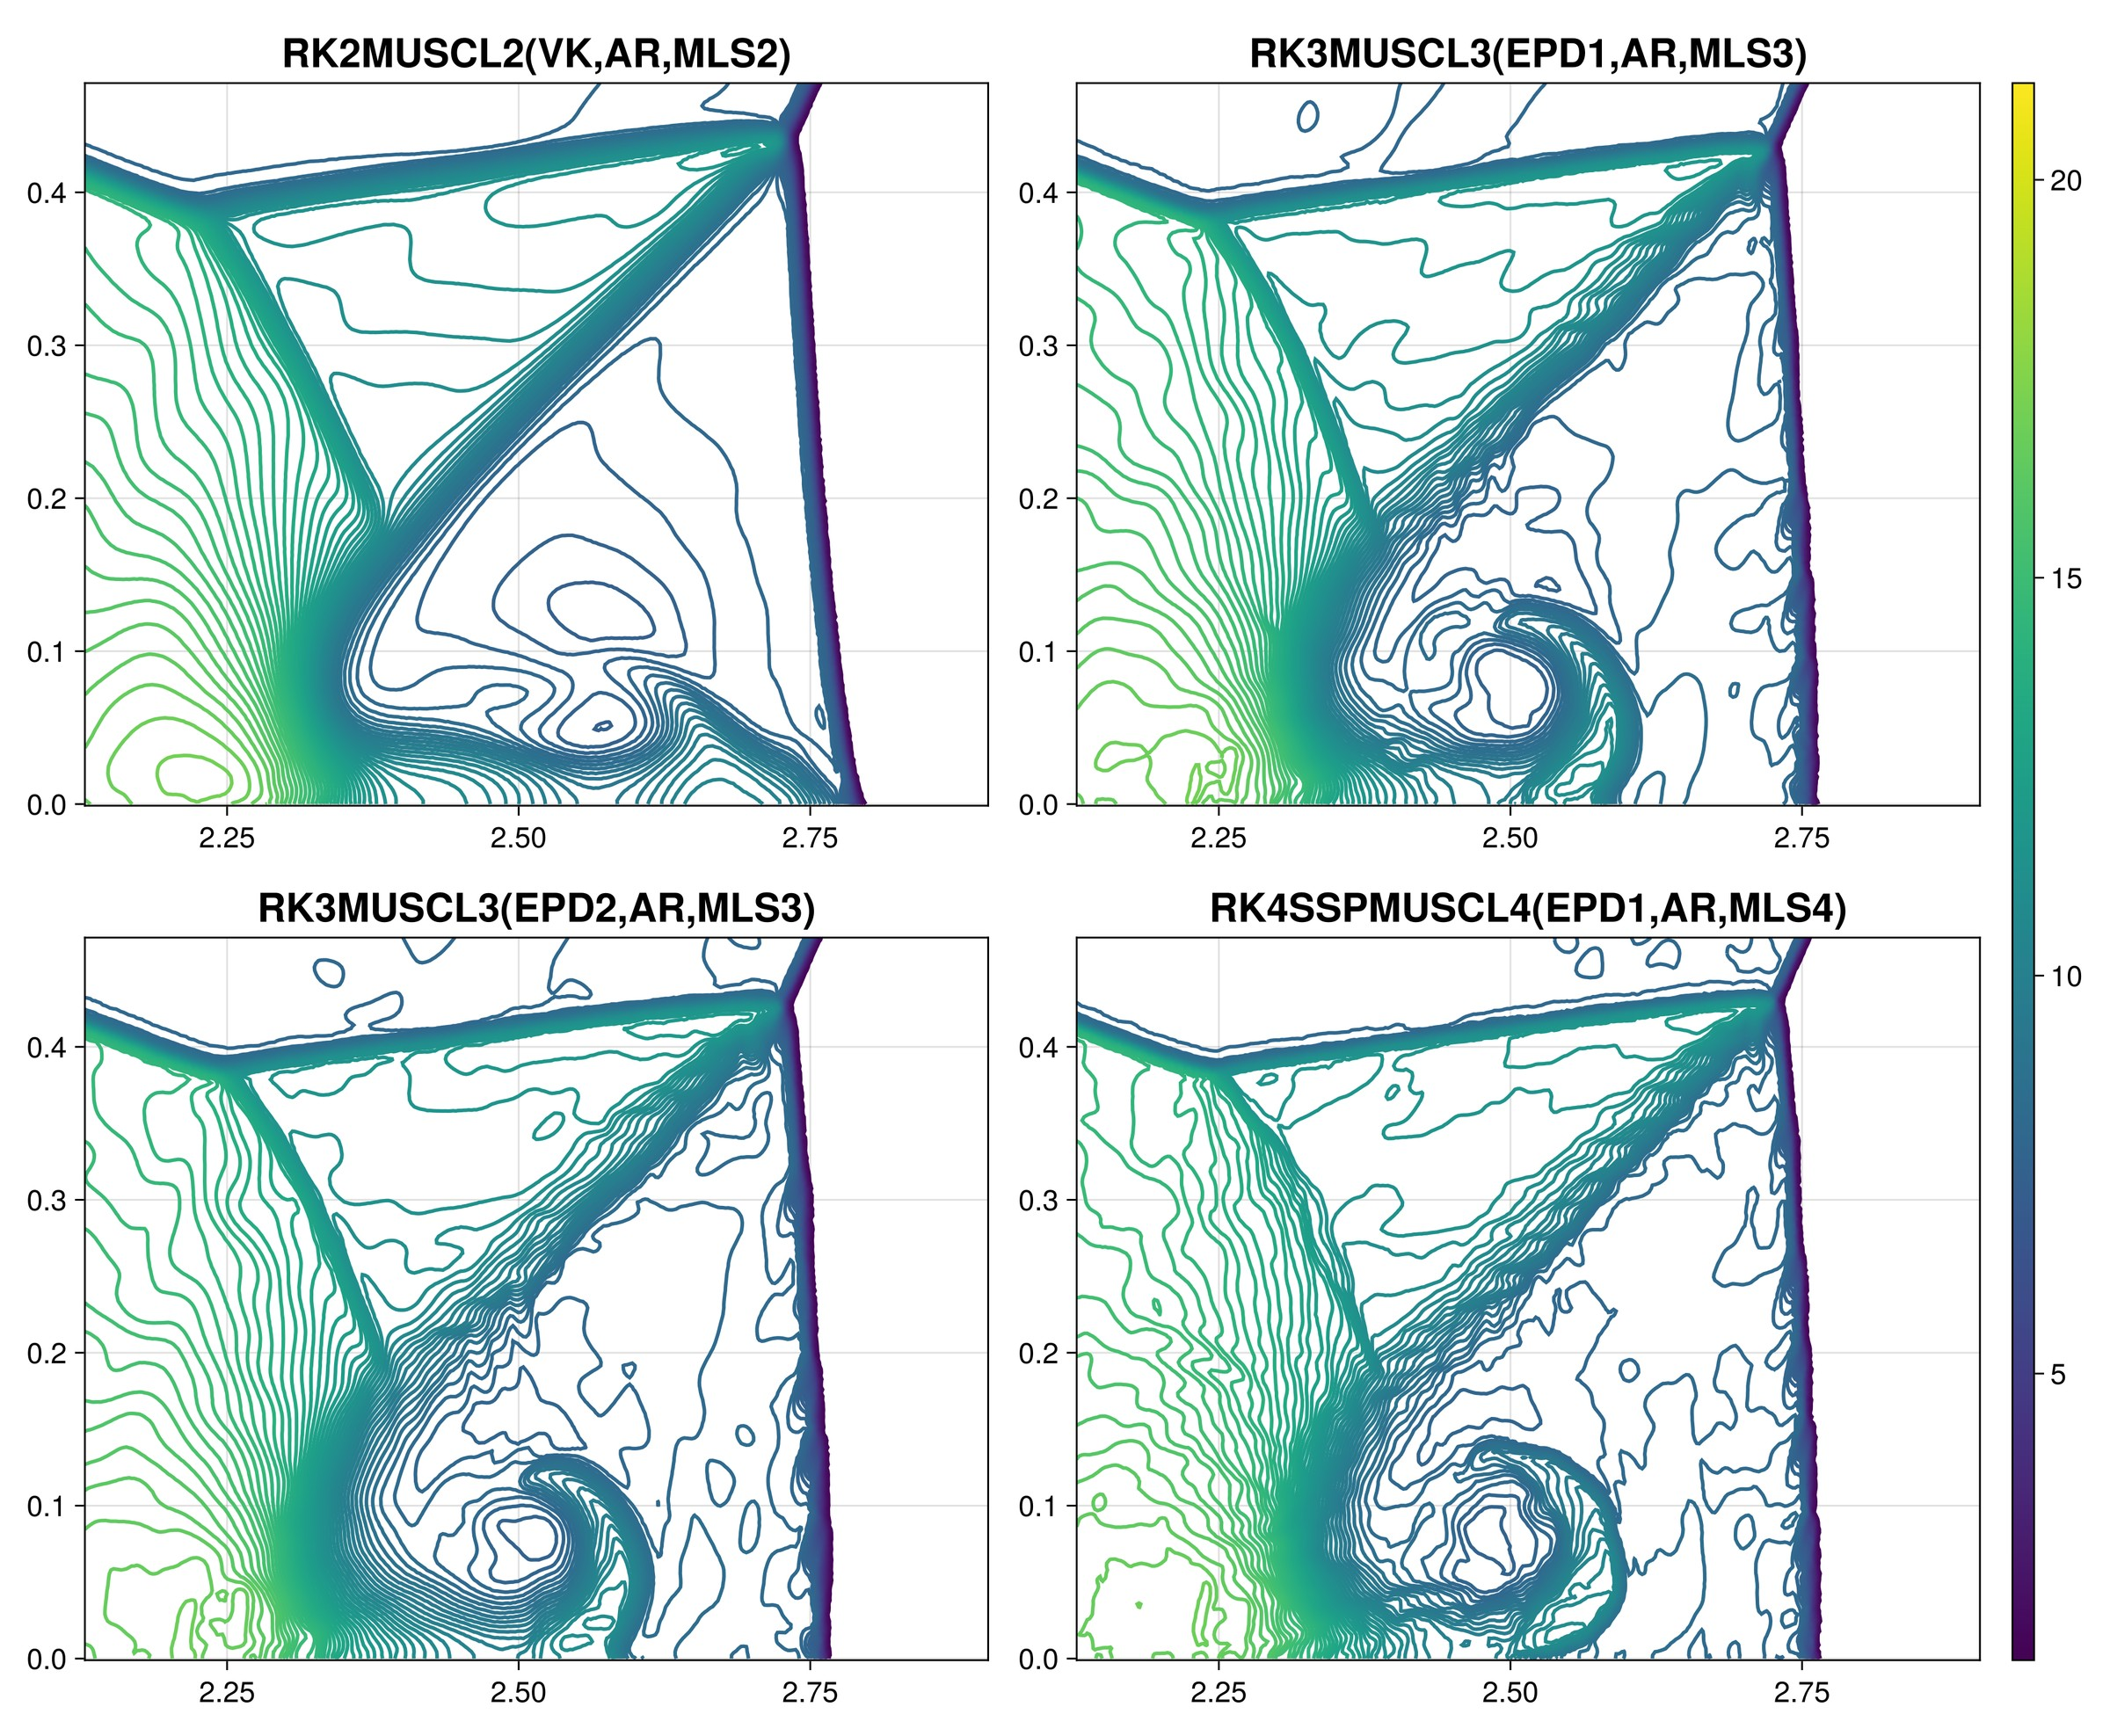
\includegraphics[width=0.85\textwidth]{figures/dmr_zoom_078.jpg}
\caption{Double Mach reflection, detail $[2.13,2.9]\times[0,0.47]$ of \cref{fig:dmr} with $100$ contour levels.}\label{fig:dmrzoom}
\end{figure}

\Cref{fig:dmr,fig:dmrzoom} show the density at $t=0.2$. All runs reproduce the characteristic pattern: the incident shock, which meets the top boundary at $x\approx3.05$, its exact position, the reflected shock, the Mach stem, the two triple points, the slip line and the wall jet. The second-order run smears the slip line, and the wall jet forms only a weak curl. The third- and fourth-order runs resolve the slip line sharply, and the jet rolls up into a vortex near $x\approx2.5$, with more structure for $K=4$ (in the reference computations the centre of this vortex moves from $x=2.56$ to $2.64$ as $h$ is refined from $1/120$ to $1/480$); the resolution of this roll-up is a common indicator of the numerical dissipation of a scheme. EPD1 and EPD2 give almost the same picture for $K=3$. The stems of the third- and fourth-order runs are almost straight at $x\approx2.76$, where the reference computations place the stem between $y\approx0.2$ and the triple point ($x\approx2.75$--$2.76$). In the second-order run the stem bends forward near the wall, to $x\approx2.79$. The reference computations show a similar bend that grows under refinement ($x=2.79$, $2.80$, $2.81$ at the wall for $h=1/120$, $1/240$, $1/480$), where the wall jet runs into the foot of the stem; the position of the foot is therefore not a converged quantity, and the bend is not by itself a defect of the second-order scheme. All runs show the highest densities at the wall near $x=\tfrac16$, where the boundary condition switches from the post-shock state to the wall; it is a start-up error caused by the discontinuous boundary data at the foot of the initial shock.

\subsection{Mach 3 wind tunnel with a step}\label{sec:step}

In the second problem of \cite{Woodward1984}, a uniform Mach 3 flow $(\rho,u,v,p)=(1.4,3,0,1)$ enters a wind tunnel of length 3 and height 1 that contains a step of height 0.2 at $x=0.6$. The tunnel is initially filled with the inflow state. The left boundary is a Dirichlet inflow, the right boundary is transmissive, and all walls, including both faces of the step, are slip walls; the ghost particles inside the step take the wall normal of the nearest face. We do not use any special treatment of the corner of the step.

\begin{figure}[!htbp]
\centering
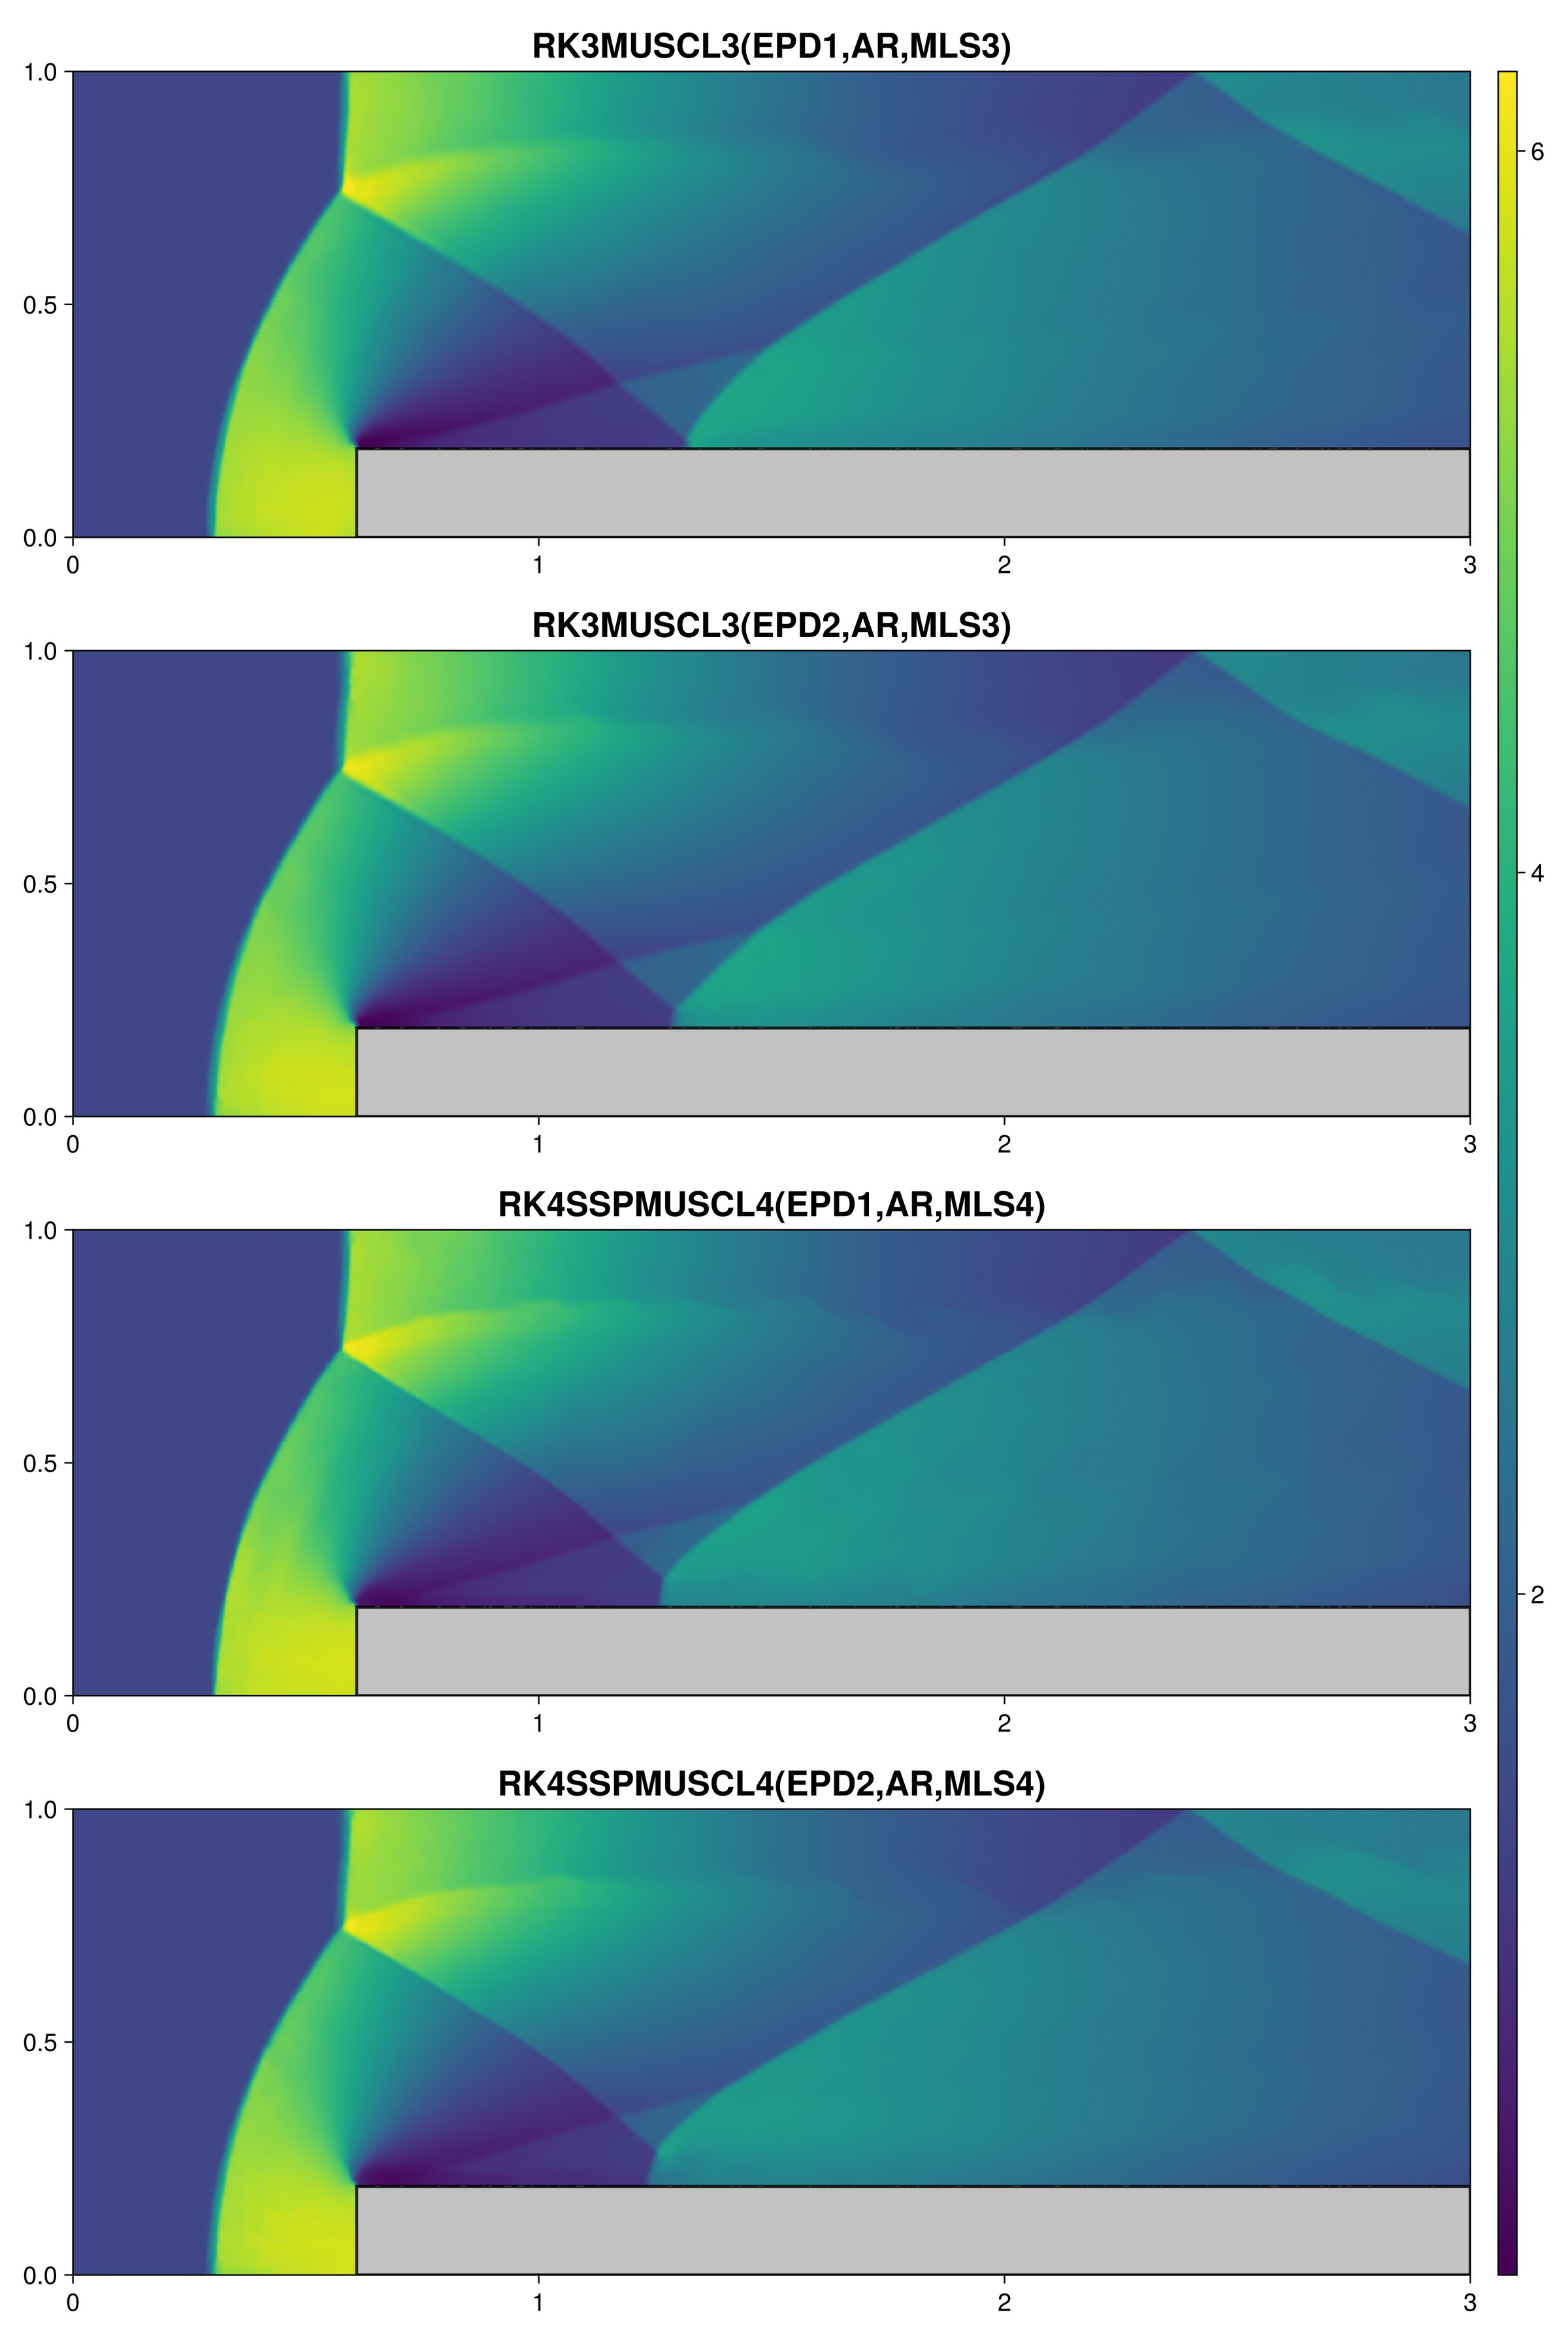
\includegraphics[width=0.68\textwidth]{figures/mach3_density_078.jpg}
\caption{Mach 3 wind tunnel with a step, density at $t=4$ on $900\times300$ particles perturbed by $0.2h$ for RK3MUSCL3 and RK4SSPMUSCL4 with EPD1 and EPD2 and $k_{\mathrm{div}}=K$, all with the aligned flux, with a common colour scale; the step is shown in grey.}\label{fig:step}
\end{figure}

\begin{table}[!htbp]
\centering
\caption{Mach 3 step: approximate wave positions at $t=4$ read from \cref{fig:step}: the bow shock at $y=0.05$, the Mach stem at $y=0.95$ and the reflection of the shock on the top of the step at $y=0.215$ (crossings of the mean of the adjacent plateau values), accurate to about $0.01$.}\label{tab:steppos}
\footnotesize
\begin{tabular}{lccc}
\toprule
& bow shock, $x$ & Mach stem, $x$ & reflection on step, $x$\\
\midrule
RK3MUSCL3(EPD1,MLS3) & 0.30 & 0.58 & 1.31\\
RK3MUSCL3(EPD2,MLS3) & 0.30 & 0.59 & 1.29\\
RK4SSPMUSCL4(EPD1,MLS4) & 0.31 & 0.59 & 1.26\\
RK4SSPMUSCL4(EPD2,MLS4) & 0.30 & 0.59 & 1.24\\
\bottomrule
\end{tabular}
\end{table}

\Cref{fig:step} shows the density at $t=4$ and \cref{tab:steppos} the positions of the main waves. All runs reproduce the bow shock in front of the step, the Mach stem at the upper wall with its triple point at $y\approx0.73$ and slip line, the expansion fan at the corner, the shock reflections at the step and the upper wall, and the wave pattern further downstream, with smooth density fields between the waves and without spurious waves. The bow shock and the Mach stem lie at the same positions in all four runs, to within $0.005$. The reflection on the step moves upstream from $x\approx1.31$ for RK3MUSCL3(EPD1) to $x\approx1.24$ for RK4SSPMUSCL4(EPD2). This position is controlled by the entropy layer at the corner: in the reference computations without a corner treatment it moves downstream under refinement ($x=1.21$, $1.24$, $1.28$ for $h=1/40$, $1/80$, $1/160$), and with a corner treatment of the type of Woodward and Colella it moves upstream ($1.39$, $1.36$, $1.34$), so that the converged position lies between about $1.28$ and $1.34$. The spread of our values thus reflects the dissipation at the corner rather than the accuracy of the interior scheme, and the two third-order runs lie within this range. The reference computations place the bow shock at $x=0.31$ at all three resolutions and the Mach stem at $x=0.62$, $0.60$ and $0.59$; our values, $0.30$--$0.31$ and $0.58$--$0.59$, agree with those of the finest reference computation to within about $0.01$. In all runs a thin region of low density lies along the top of the step behind the corner; without a special treatment of the corner this is where the entropy layer forms that Woodward and Colella suppressed \cite{Woodward1984}. Cockburn and Shu \cite{CockburnShu1998}, who also use no special treatment of the corner, observe that this layer shrinks under refinement.

\subsection{Discussion}\label{sec:discussion}

The test problems are demanding even for conservative FV schemes on Cartesian meshes. In the double Mach reflection the resolution of the slip line and of the roll-up of the wall jet is a sensitive measure of numerical dissipation, the discontinuous boundary data at the beginning of the wall cause a start-up error, and Roe's Riemann solver, whose dissipation is low, can produce a kinked Mach stem \cite{Quirk1994}. In the step problem the corner is a singular point of the flow, and without a special treatment an entropy layer develops along the top of the step \cite{Woodward1984}. Our scheme faces these difficulties without the structural advantages of FV methods: it is not exactly conservative (\cref{sec:conservation}), its stencils are irregular and overlapping, and its walls are represented by ghost particles with first-order boundary states. Against this background the results are robust. For smooth solutions the schemes attain their design orders up to five on lattices and on perturbed clouds. With the aligned flux every shock computation completes with positive density and pressure, in single precision and without any problem-specific treatment, and with the full derivative degree the third- and fourth-order schemes resolve slip lines and roll-ups markedly better than the second-order scheme.

Three ingredients make the schemes work. First, the derivative degree $\qdiv(k)$ of \eqref{eq:qk} is odd, so that the leading flux errors cancel on symmetric stencils and the truncation error is of order $k$ on lattices (\cref{sec:consistency}); the observed convergence orders are an experimental result; with the even degree $k-1$ the odd orders would lose one order. The analysis covers symmetric stencils only, but the convergence studies show the same orders on clouds perturbed by $0.2h$ whenever the stencils are large enough for the fits (\cref{sec:smooth}). Second, the aligned orientation of the Rusanov dissipation keeps the first-order fallback positive for derivative weights of any degree. With the geometric orientation, about $40\%$ of the degree-three weights turn the dissipation of a lowered particle into anti-dissipation (\cref{sec:positivity}), so that with this orientation the fallback of the fourth-order scheme with $k_{\mathrm{div}}=4$ is not positive; with the aligned orientation it runs on all shock problems. Third, MOOD checks the forward Euler substeps of the SSP methods, so that every Runge--Kutta stage is a convex combination of checked states (\cref{sec:stagemood}).

The aligned flux removes the trade-off between a positive fallback and conservation. The positivity of the first-order scheme follows from the orientation of the dissipation (\cref{sec:positivity}) instead of the degree of the derivative operator, so the degree can stay the same for all particles, and the pairs of different degrees, whose conservation defect does not decrease under refinement, do not occur. The coupled mode, which keeps these pairs, is positive as well, but it changes the mass by several percent and is not competitive. What remains in the frozen mode is the static asymmetry of the weights on irregular clouds, whose effect decreases under refinement also at moving shocks (\cref{sec:mass}). The price is more dissipation at lowered particles with high-degree weights and, for $k_{\mathrm{div}}\ge3$, a three times smaller time step. The frozen mode with $k_{\mathrm{div}}=K$ keeps the formal order, is positive on all problems, resolves the most structure and leaves smooth extrema alone from coarser resolutions on, at three times the cost of the second-order scheme. With $k_{\mathrm{div}}=2$ the frozen mode costs as much as the second-order scheme and conserves to the floor of all tests, but by \cref{sec:consistency} it is formally of second order in smooth regions, although its reconstructions are of higher degree, which the isentropic vortex confirms. The two interface rules trade accuracy for robustness. EPD1 is less dissipative: for $K=3,4$ with $k_{\mathrm{div}}=2$ its Sod errors are $1.6$ to $1.8$ times smaller than those of EPD2, and it keeps the density maximum next to the jet of the Riemann problem, which EPD2 smears; with $k_{\mathrm{div}}=K$ the two rules give almost the same accuracy on the Sod problem and the double Mach reflection. EPD2 is more robust near strong shocks at walls: on the step with $k_{\mathrm{div}}=K$ its minimum pressures are $0.081$ ($K=3$) and $0.28$ ($K=4$), against $0.0048$ and $0.034$ with EPD1, and at $K=4$ its conservation defect at the moving shock decreases under refinement, whereas that of EPD1 stays at about $10^{-3}$ in the range tested.

The isentropic vortex shows that MOOD has to be adapted to meshfree stencils to leave smooth flows alone: with a plateau test for components without structure at the scale of the stencil, and with the curvature magnitudes compared among the nearest neighbours only, MOOD (with EPD2; EPD1 was not tested on the vortex) keeps the vortex core for $K\ge3$ once the core is resolved by about ten ($k_{\mathrm{div}}=K$) to twenty ($k_{\mathrm{div}}=2$) particles per radius (\cref{sec:vortex}). The plateau threshold is relative to the global range of the solution and has to be larger on coarse clouds, and for $K=2$ smooth extrema are still clipped. Limitations are the reduced order of $K=4$ on perturbed clouds with the small radius $\kappa=2.5$, a possible round-off floor of high-order fits in single precision, and the first-order ghost-particle boundary conditions. For the present code we recommend the frozen mode with the aligned flux, with $k_{\mathrm{div}}=K$ for the full formal order and $k_{\mathrm{div}}=2$ where cost matters more than the formal order, and MOOD with EPD1 for less dissipation or EPD2 for more robustness.

% ===========================================================================
\section{Open questions and further studies}\label{sec:open}
% ===========================================================================

The experiments raise a number of questions that we leave to future work.
\begin{itemize}
\item \emph{Smooth-extremum detection.} The plateau test and the revised u2 criterion keep the core of the isentropic vortex for $K\ge3$. Open are a plateau threshold that does not depend on the global range and the resolution, a smooth-extremum test for $K=2$, curvature tests on characteristic or primitive variables, and the behaviour on smooth flows with extrema of several components at once.
\item \emph{Conservation.} With the aligned flux and the frozen degree-one derivative operator the conservation defect decreases under refinement. Constructing antisymmetric face vectors \cite{Chiu2012} would remove it, and constraining the weights to approximately antisymmetric ones \cite{Suchde2017} would reduce it; and with the aligned orientation such weights would keep a positive fallback. It remains open why the frozen mode with $k_{\mathrm{div}}=K\ge4$ and EPD1 keeps defects of $10^{-3}$ to $7\cdot10^{-3}$ that decrease slowly or not at all, and how the defect depends on $h$ in general.
\item \emph{Interface reconstructions.} Lower interface orders truncate the existing fit instead of refitting (\cref{sec:recfit}); whether a refit per interface improves the results at discontinuities, and at what cost, is open; for whole cells, FV-MOOD schemes abandoned truncation for degrees above two \cite[Remark~4]{Diot2012}.
\item \emph{Symmetry of the aligned flux.} On perturbed clouds the two particles of a pair use different fluxes on the pairs whose weights have equal signs (\cref{sec:fluxes}). A symmetric choice, for instance by the sign of $V_ic_{ij}-V_jc_{ji}$, would keep the positivity argument only approximately; whether it improves conservation is open.
\item \emph{Stencils and precision.} The full order of $K=4$ on perturbed clouds with $\kappa=2.5$, adaptive radii, and a possible round-off floor of the high-order fits in single precision.
\item \emph{Boundary conditions.} Ghost states at reflected positions instead of nearest-donor copies would raise the order at walls.
\item \emph{Further tests.} Refinement studies of the shock problems against converged reference solutions, which would also decide the differences between the high-order runs on the step, the Lax and Shu--Osher problems, and three-dimensional problems.
\end{itemize}

% ===========================================================================
\section{Conclusions}\label{sec:conclusion}
% ===========================================================================

We have presented meshfree MUSCL schemes of arbitrary design order for hyperbolic systems on scattered point clouds. Midpoint Riemann problems between MLS reconstructions, combined with an MLS derivative operator with zero row sums, give an update in terms of interface fluxes only. The scheme is exact for polynomial solutions of degree $k-1$ of linear problems, the degree of the derivative operator follows from a parity argument, and the conservation error reduces to the lack of antisymmetry of the volume-weighted derivative weights. A~priori limiters and a stage-wise MOOD procedure with physical and numerical admissibility detection and three interface rules control oscillations. Orienting the Rusanov dissipation by the signs of the derivative weights makes the first-order fallback positive for derivative operators of any degree, so that the derivative degree can stay uniform while MOOD lowers the reconstruction degrees, which removes the pairs of mixed degrees that dominated the conservation error.

The numerical experiments show that these schemes are a promising and robust basis for high-order meshfree computations of compressible flows. For smooth solutions they attain their design orders two to five on lattices and on perturbed clouds. With a derivative operator of degree one the conservation defect at moving shocks decreases under refinement and reaches the resolution of the tests; with higher degrees it is small but, for $K=4$ with EPD1 and for $K=5$, decreases slowly or not at all. On the double Mach reflection, the Mach~3 step and a two-dimensional Riemann problem on perturbed clouds of up to $6.5\times10^5$ particles, all computations complete with positive density and pressure, in single precision, reproduce the characteristic wave patterns without spurious waves apart from start-up errors, and with the full derivative degree the high-order schemes resolve fine structures markedly better than the second-order scheme. With a plateau test and a smooth-extremum detection adapted to meshfree stencils, MOOD leaves the core of the isentropic vortex intact for the orders three and four once the core is resolved by ten to twenty particles per radius, and checking the forward Euler substeps of the SSP methods makes every Runge--Kutta stage a convex combination of checked states. The limitations we observed are the reduced order of the fourth-order scheme on perturbed clouds with small stencils, the clipping of smooth extrema by MOOD at order two, and the low-order ghost-particle boundary conditions.

The natural next steps are weights with (approximately) antisymmetric face vectors \cite{Chiu2012,Suchde2017}, and higher-order boundary conditions (\cref{sec:open}). The implementation \cite{jung_hypercloudcore,jung_hypercloud} already supports moving clouds in an arbitrary Lagrangian--Eulerian setting, implicit--explicit time integration, three-dimensional problems and GPUs, which will allow applications to physical problems with a more mature version of the method.

\section*{Software}
The schemes are implemented in HyperCloudCore.jl \cite{jung_hypercloudcore} (version 0.7.8; all results of \cref{sec:experiments}), the test cases are run with HyperCloud.jl \cite{jung_hypercloud} (version 0.5.1), and the figures were produced with PDEStudio \cite{jung_pdestudio} (version 0.4.5). The run configurations and the driver scripts of all experiments are in \cite{jung_meshfree_simulations}.
HyperCloudCore.jl was developed over roughly 18 months with AI assistance whose form changed over the project. In the earlier phase, Gemini models, mostly 3.1 Pro, were used interactively to draft code, explain errors, and suggest implementations, and the first author adapted and integrated this output by hand. From commit 2e4e6fb970 (14.10.2026) onward, most code changes were written with Claude Fable 5.1 in Claude Code, and each change was submitted as a pull request that the first author reviewed manually before merging. Because the two modes were interleaved with the first author's own programming, no precise per-component attribution is given. The correctness of the solver as a whole was established independently of the AI tooling through the convergence studies and benchmarks found in \cref{sec:experiments}. All numerical results in this paper come from executing the code. The full development history is available at \url{https://github.com/industrial-mathematics-group/HyperCloudCore.jl}.
The finite-volume reference computations of \cref{sec:riemann,sec:dmr,sec:step} use a separate Python code (Numba-accelerated; MUSCL reconstruction of the primitive variables with the MC limiter, HLLC flux, SSP-RK3 on uniform Cartesian grids, solid walls by mirror cells). It was written with Claude Fable 5.1 (Anthropic) in Claude Code for this paper, checked against the exact plane-shock positions of the Riemann problem and the incident shock of the double Mach reflection, and is released together with the data as supplementary material.
\appendix
% ===========================================================================
\section{Options of the scheme}\label{app:options}
% ===========================================================================

\Cref{tab:options} summarizes the options of the scheme as covered in this paper and the corresponding settings of HyperCloud.jl.

\begin{table}[!htbp]
\centering
\caption{Options of the meshfree MUSCL scheme with explicit time integration.}\label{tab:options}
\small
\begin{tabular}{>{\raggedright\arraybackslash}p{3.4cm}>{\raggedright\arraybackslash}p{6.2cm}>{\raggedright\arraybackslash}p{4.6cm}}
\toprule
component & options & HyperCloud setting\\
\midrule
design order $K$ & $K\ge1$; reconstruction degree $K-1$, derivative degree $\qdiv(K)$ & \texttt{Scheme\_order}\\
derivative mode & coupled ($q_i=\qdiv(k_i)$) or frozen ($q_i=\qdiv(k_{\mathrm{div}})$) & \texttt{Scheme\_MLS\_order} $=0$ or $k_{\mathrm{div}}$\\
numerical flux & Rusanov with geometric or aligned orientation; upwind (scalar equations) & \texttt{Flux\_name} $=$ \texttt{Rusanov}, \texttt{AlignedRusanov}, \texttt{Upwind}\\
a~priori limiter & none, BJ, VK; minmod, superbee (1-D); hard or soft & \texttt{Limiter\_name}, \texttt{Limiter\_mode}\\
MOOD criterion & none; DMP \eqref{eq:dmp}; DMP with plateau test ($\pi_0$) and u2 \eqref{eq:u2} (ratio $\tfrac12$); PAD always with MOOD & \texttt{MOOD\_criterion}, \texttt{MOOD\_delta\_relax} $=\delta_0$; \texttt{plateau}, \texttt{curvature\_ratio}\\
interface rule & EPD0, EPD1, EPD2 & \texttt{MOOD\_strategy}\\
time integration & forward Euler, RK2 (SSP), Ralston, RK3 (SSP), RK4, SSPRK(5,4); orders reset per step or per stage; MOOD checks the Euler substeps (default) or the stage candidates & \texttt{Time\_stepper}, \texttt{Time\_reset\_orders\_}\allowbreak\texttt{per\_stage}; \texttt{mood\_substeps}\\
time step & $\CFL$ in \eqref{eq:cfl} or fixed $\Delta t$ & \texttt{Time\_CFL}, \texttt{Time\_dt}\\
weights, support & \eqref{eq:weight} with $\alpha$, or $w(r)=1/(r^2+10^{-12})$; $R=\kappa h$ & \texttt{Weight\_name}, \texttt{Weight\_alpha}, \texttt{Weight\_range}\\
\bottomrule
\end{tabular}
\end{table}

% ===========================================================================
\section{Stencil diagnostics}\label{app:stencils}
% ===========================================================================

\Cref{tab:stencils} collects the properties of the derivative weights on the clouds of \cref{sec:experiments} that are quoted throughout the paper: the size of the weights, the share of weights whose sign differs from that of the offset (which matters for the orientation of the Rusanov flux, \cref{sec:fluxes,sec:positivity}), and the pair defects that determine the conservation error (\cref{sec:conservation}).

\begin{table}[!htbp]
\centering
\caption{Stencil diagnostics for the clouds of \cref{sec:experiments} ($\kappa=2.5$, weight \eqref{eq:weight} with $\alpha=1$, Shepard volumes after one smoothing sweep; without the sweep the pair defects for equal degrees are $6.2\%$ and $16.9\%$ on the perturbed lattice): a periodic lattice and a periodic $300\times300$ lattice with a random perturbation of amplitude $0.2h$ per coordinate. Per-particle quantities are means over the particles with the maxima in parentheses; the shares of entries and of particles and the pair defects $\sum|V_ic_{ij}+V_jc_{ji}|/\sum(|V_ic_{ij}|+|V_jc_{ji}|)$ are global ratios. Computed with an independent NumPy implementation of the fits (script provided as supplementary material).}\label{tab:stencils}
\small
\begin{tabular}{lcccc}
\toprule
& \multicolumn{2}{c}{lattice} & \multicolumn{2}{c}{perturbed lattice}\\
\cmidrule(lr){2-3}\cmidrule(lr){4-5}
derivative degree $q$ & 1 & 3 & 1 & 3\\
\midrule
neighbours per particle & 20 & 20 & 19.6 (16--22) & 19.6 (16--22)\\
$\ell^1$ norm $h\sum_{j,d}|c^{(d)}_{ij}|$ & 1.36 & 3.59 & 1.40 (1.57) & 3.79 (4.72)\\
\quad the same without constant term & 1.36 & 3.59 & 1.40 (1.55) & 3.79 (4.65)\\
\quad largest relative difference & 0 & 0 & 3.5\% & 10.6\%\\
row sum without constant term, $|\sum_j\hat c_{ij}|/\sum_j|\hat c_{ij}|$ & 0 & 0 & 4.3\% (18.9\%) & 4.0\% (18.5\%)\\
entries with $\sgn(x_{ij,d})\,c^{(d)}_{ij}<0$ & 0 & 40\% & 3.2\% & 44\%\\
particles with such entries & 0 & 100\% & 72\% & 100\%\\
share of these entries in $\sum_{j,d}|c^{(d)}_{ij}|$ & 0 & 17.5\% & 0.17\% (4.8\%) & 18\% (28\%)\\
pair defect, equal degrees & 0 & 0 & 5.3\% & 16.6\%\\
pair defect, degrees 1 and 3 & \multicolumn{2}{c}{73\%} & \multicolumn{2}{c}{73\%}\\
pairs and directions with $c^{(d)}_{ij}c^{(d)}_{ji}>0$ & 0 & 0 & 5.0\% & 19\%\\
\quad their share in $\sum(|c^{(d)}_{ij}|+|c^{(d)}_{ji}|)$ & 0 & 0 & 0.4\% & 4.7\%\\
\bottomrule
\end{tabular}
\end{table}


\section*{Acknowledgements}
The computations were carried out on the high-performance cluster Elwetritsch of the Regional University Computing Center Kaiserslautern-Landau (RHRZ) at RPTU. This work was funded by the Deutsche Forschungsgemeinschaft (DFG, German Research Foundation).

\section*{Declaration of generative AI use}
Declaration of generative AI and AI-assisted technologies in the manuscript preparation process. During the preparation of this work, the first author used Claude Opus 5.5 (Anthropic) to draft substantial parts of the manuscript text. The supplementary material, i.e.\ the mathematical companion with the proofs, the stability note, the analysis scripts and the finite-volume reference code, was generated with Claude Fable 5.1 (Anthropic) in Claude Code, and the tables of the run reports were compiled with Claude Opus 5.5. These parts and the manuscript were reviewed by independent Claude Opus 5.5 sessions without access to the generating conversations, which re-derived the proofs and reran the scripts and reference computations. The authors reviewed, revised, and verified all content, including every reference and every numerical claim, and take full responsibility for the content of this publication.

\bibliographystyle{plainnat}
\bibliography{refs}

\end{document}
